\documentclass[11pt]{article}
\usepackage[T1]{fontenc}
\usepackage[utf8]{inputenc}
\usepackage{lmodern}
\usepackage[a4paper,margin=28mm]{geometry}
\usepackage{amsmath,amssymb,amsthm,mathtools}
\usepackage{enumitem,booktabs,array}
\usepackage{microtype}
\usepackage{xcolor}
\usepackage[hyphens]{url}
\usepackage{tikz}
\usetikzlibrary{arrows.meta,positioning,calc,decorations.pathreplacing}
\usepackage{hyperref}
\hypersetup{colorlinks=true,linkcolor=blue!45!black,citecolor=blue!45!black,
  urlcolor=blue!45!black,pdfauthor={OpenAI},
  pdftitle={Nonhomeomorphic closed aspherical four-manifolds with the same homotopy type}}
\newtheorem{theorem}{Theorem}[section]
\newtheorem{proposition}[theorem]{Proposition}
\newtheorem{lemma}[theorem]{Lemma}
\newtheorem{corollary}[theorem]{Corollary}
\theoremstyle{definition}
\newtheorem{definition}[theorem]{Definition}
\newtheorem{convention}[theorem]{Convention}
\theoremstyle{remark}
\newtheorem{remark}[theorem]{Remark}
\numberwithin{equation}{section}
\setlist[enumerate]{label=\textup{(\roman*)},leftmargin=*}
\setlist[itemize]{leftmargin=*}
\newcommand{\Ftwo}{\mathbb F_2}
\DeclareMathOperator{\Aut}{Aut}
\DeclareMathOperator{\Out}{Out}
\DeclareMathOperator{\Inn}{Inn}
\DeclareMathOperator{\lk}{lk}
\DeclareMathOperator{\st}{st}
\DeclareMathOperator{\supp}{supp}
\DeclareMathOperator{\wt}{wt}
\newcommand{\manuscriptid}[1]{\begingroup\Urlmuskip=0mu plus 2mu\nolinkurl{#1}\endgroup}
\title{Nonhomeomorphic closed aspherical four-manifolds\\
with the same homotopy type}
\author{OpenAI}
\date{October 4, 2026}
\begin{document}
\maketitle
\begin{abstract}
We construct closed connected aspherical topological four-manifolds
that are homotopy equivalent but not homeomorphic, disproving the
homeomorphism-existence formulation of the Borel conjecture in dimension
four.  Their common
fundamental group is word-hyperbolic.  One of the manifolds also has a
self-homotopy equivalence not homotopic to a homeomorphism.
\end{abstract}
\section{Introduction}\label{sec:introduction}

A connected manifold is \emph{aspherical} if its universal cover is
contractible.  Its fundamental group then determines its homotopy type.
The topological Borel conjecture commonly asks whether every homotopy
equivalence between closed aspherical manifolds is homotopic to a
homeomorphism \cite{BartelsLueck2012,Lueck2010}.  The weaker
\emph{homeomorphism-existence formulation} asks only whether
homotopy-equivalent closed aspherical manifolds are homeomorphic.
Our main result disproves this formulation in dimension four.

\begin{theorem}\label{thm:pair}
There exist closed connected aspherical topological four-manifolds
$M$ and $N$ that are homotopy equivalent but not homeomorphic.
Their common fundamental group is word-hyperbolic.
\end{theorem}

The conclusion excludes every homeomorphism between the two manifolds,
without prescribing a homotopy class.  The construction also yields a
separate obstruction for a self-map of one manifold.

\begin{theorem}\label{thm:self-map}
There exist a closed connected aspherical topological four-manifold
$M$ and a homotopy equivalence $f\colon M\to M$ such that no
homeomorphism $M\to M$ is homotopic to $f$.
\end{theorem}

We prove this assertion separately and use the same $M$ in
Theorem~\ref{thm:pair}.  A nonhomeomorphic pair alone would not imply
the self-map assertion.

The homeomorphism-existence question already appears in Borel's letter
to Serre of May~2, 1953, phrased for compact manifolds that are
classifying spaces \cite{Borel1953}.  Rigidity holds classically in
dimensions at most two, and for closed orientable aspherical
three-manifolds by geometrization and three-dimensional rigidity
\cite[Theorem~0.7 and Section~5]{KreckLueck2009}.
In higher dimensions, Hsiang and Wall proved the homeomorphism-existence
statement for homotopy tori in dimensions at least five
\cite{HsiangWall1969}, and Farrell and Jones established it for closed
negatively curved manifolds in those dimensions
\cite{FarrellJones1989}.  Bartels and L\"uck proved the prescribed-class
formulation in dimensions at least five for a class of groups containing
word-hyperbolic groups and groups acting geometrically on
finite-dimensional CAT(0) spaces \cite[Theorem~A]{BartelsLueck2012}.

In dimension four, these rigidity theorems use further geometric input.  Bartels and
L\"uck's four-dimensional application assumes that the fundamental
group is good in the sense of Freedman
\cite[Proposition~0.3]{BartelsLueck2012}.  For closed aspherical
topological four-manifolds with torsion-free word-hyperbolic fundamental
group, Khan proves rigidity up to topological $s$-cobordism
\cite[Theorem~1.22 and Corollary~1.23]{Khan2012}; the product theorem for
five-dimensional topological $s$-cobordisms in Freedman--Quinn assumes
a good fundamental group \cite[Theorem~7.1A]{FreedmanQuinn1990}.
The word-hyperbolicity in Theorem~\ref{thm:pair} therefore lies within
the group-theoretic range of these rigidity results, while the
dimension is essential to their topological conclusion.  Recent
examples of Davis, Hayden, Huang, Ruberman, and Sunukjian are closed
aspherical smooth four-manifolds that are homeomorphic but not
diffeomorphic \cite[Theorem~1.1]{DHHRS2026}.  Their proof uses Davis
reflection and a characteristic-subgroup argument to force a hypothetical
diffeomorphism between these manifolds to lift to covers distinguished by
the genera of smoothly embedded homologically essential surfaces
\cite{DHHRS2026}.  Our conclusion concerns
homeomorphism in the topological category.

The proof uses two companion constructions.  The marked tensor
obstruction of \cite{MT} supplies plumbing blocks, marked grope bodies,
and algebraic potentials associated to three-dimensional cuts.  The
reflection and realization results of \cite{PD} turn the absence
of a marked filling into the absence of a closed manifold model for
an aspherical Poincar\'e complex.  We also use its universal-development and support arguments.
We state the imported results at their points of use and verify their
hypotheses for the chambers constructed here.  The principal inputs
are the marked algebraicity theorem \cite[Theorem~5.1]{MT}, the
controlled filling implication \cite[Sections~3--5]{PD}, and the
support construction \cite[Lemma~3.3]{PD}.

\subsection*{The construction}

Start with a finite collared Poincar\'e chamber $(P,S)$ of dimension
four, where $P$ has the homotopy type of a finite graph and its
fundamental group has an epimorphism to $\mathbb Z$.  Write $S_d$ for
the boundary in the connected cyclic cover of degree $d$.  A
\emph{marked filling} of $S_d$ is a compact four-manifold with this
identified boundary and the prescribed graph homotopy type, including
the boundary map.  The double cover $S_2$ has a marked filling, whereas
$S_d$ has none for odd $d\geq3$.

This parity comes from two colors of plumbing caps.  Each grope has
four terminal caps grouped into two red--blue pairs.  In the double
cover, choosing red caps at one vertex and blue caps at the other
makes the selected sheets disjoint and gives the filling.  For odd
$d\geq3$, a hypothetical filling of $S_d$ instead produces formal data
on a cycle of $d$ vertices with five red and five blue edges between
each neighboring pair.  The endpoint-assignment theorem would assign
every edge to one endpoint so that each vertex receives at most one
edge in some color.  Choose one such color at each vertex.  Adjacent
vertices cannot choose the same color, since together they would receive
at most two of the five edges of that color between them.  The choices
would alternate around the cycle, impossible when the cycle is odd.

We formulate the endpoint-assignment theorem for arbitrary finite
loopless multigraphs.
The cyclic-cover criterion works in every manifold dimension.  It
converts a double-cover model and eventual nonexistence of odd-cover
models into a self-homotopy equivalence not represented by any
homeomorphism.  The proof composes a lifted homeomorphism with a large
deck translation and imposes no finite-order condition on that
homeomorphism.  This last distinction separates the criterion from
finite-group Nielsen realization obstructions such as
\cite[Theorem~1.6]{BlockWeinberger2008}.

To construct the pair, use the reflection method of Davis
\cite{Davis1983,Davis2008} in the Poincar\'e-chamber form of
\cite{PD}.  A full reflection of $P$ has no manifold model in its
cyclic covers of odd degree $d\geq3$.  We quotient its elementary abelian
group of chamber labels by a binary relation space that acts freely
and forces every
simplicial symmetry preserving the relations to be trivial.  The
quotient is a finite aspherical complex $Q$ with the same odd-cover
obstruction.

There are two ways to replace the chambers of $Q_2$ by the filling of
$S_2$.  In one, every boundary identification is the same.  In the
other, it is twisted by the double-cover deck involution according to
a nonzero linear functional $\ell$ on the label group $\mathsf A$.
Both gluings are closed manifold models of $Q_2$.  They realize two
subgroups of outer automorphisms of the common group $\Pi$:
the horizontal subgroup $\mathsf A$ on $M$ and the graph subgroup
$\mathsf B_\ell$ on $N$.  These lie in
$\mathsf A\times\langle\delta\rangle\leq\Out(\Pi)$, where $\delta$ is
the cyclic involution.  The cyclic-cover criterion forbids $\delta$
on $M$ and at the same time proves Theorem~\ref{thm:self-map}.
The subgroups $\mathsf A$ and $\mathsf B_\ell$ are not conjugate in
$\Out(\Pi)$: they contain different numbers of elements admitting
finite-order lifts to $\Aut(\Pi)$.

The remaining step controls all possible homotopy classes of a
homeomorphism between the models.  We prove that $\Out(\Pi)$ is finite:
a uniform bound on square grids makes the support cubulation
hyperbolic, and Poincar\'e duality with the homological Shapiro lemma
excludes the virtually cyclic splittings forced by an infinite outer
automorphism group.  A direct rigidity argument for the right-angled
Coxeter group of the infinite lifted triangulation then gives
\[
 N_{\Out(\Pi)}(\mathsf A)=\mathsf A\times\langle\delta\rangle.
\]
The normalizer equality and the absence of $\delta$ make
$\mathsf A$ a Sylow $2$-subgroup of the outer automorphisms realized on
$M$.  A homeomorphism from $M$ to $N$ would transport
$\mathsf B_\ell$ into that realized group and force the forbidden
conjugacy.  This proves Theorem~\ref{thm:pair}.

Section~\ref{sec:cyclic} gives the two realization criteria.
Section~\ref{sec:reflection} states the chamber data and derives the
reflected odd-cover obstruction.  Sections~\ref{mod:section}
and~\ref{ext:section} construct the two models and identify their
outer actions.  Sections~\ref{hyp:section} and~\ref{nor:section}
prove the group-theoretic statements and the main theorem.
Finally, Sections~\ref{sec:chambers}--\ref{sec:formal} prove the
chamber data, including the general tensor theorem and the odd-cover
obstruction.

All manifolds are connected unless otherwise indicated.  Boundaries
have collars, and cornered constructions are rounded.  Homotopies
of markings are part of the data when boundary maps are prescribed.
We use singular cohomology unless a differential-form model is
specified, and write $\Gamma_j F$ for the lower central series of
a group $F$.

\section{Cyclic covers and realized symmetries}\label{sec:cyclic}

Two criteria organize the passage from a filling obstruction to the
homeomorphism conclusions.  The first forbids a prescribed outer
automorphism from being induced by a homeomorphism.  The second uses
finite symmetry groups to distinguish two manifold models without
prescribing the homotopy class of a possible homeomorphism.

\subsection{A criterion from cyclic covers}

We first isolate the passage from manifold existence in finite covers to
a homotopy equivalence that cannot be represented by a homeomorphism.
This passage is independent of the four-dimensional construction.
A \emph{closed topological $n$-manifold model} of a space is a closed,
connected topological $n$-manifold equipped with a homotopy equivalence
to that space.

\begin{theorem}[Cyclic-cover criterion]\label{cyc:criterion}
Let $Q$ be a connected finite aspherical CW complex, put
$G=\pi_1(Q)$, and let $w\colon G\twoheadrightarrow\mathbb Z$ be an
epimorphism.  For every positive integer $d$, write
\[
 G_d=w^{-1}(d\mathbb Z)
 \qquad\text{and}\qquad
 Q_d\longrightarrow Q
\]
for the associated connected cyclic cover.  Fix an integer $n\geq1$.
Suppose that $Q_2$ has a closed topological $n$-manifold model $M$, but
that $Q_d$ has no such model for every sufficiently large odd integer
$d$.

Choose $\gamma\in G$ with $w(\gamma)=1$, and use the model equivalence
to identify $\pi_1(M)$ with $G_2$.  The outer automorphism of $G_2$
represented by
\[
 \alpha(g)=\gamma g\gamma^{-1}
\]
is induced by a self-homotopy equivalence of $M$.  No homeomorphism of
$M$ induces this outer automorphism.  In particular, that
self-homotopy equivalence is not homotopic to a homeomorphism.
\end{theorem}

\begin{proof}
The manifold $M$ is aspherical, since it is homotopy equivalent to
$Q_2$.  Topological manifolds have CW homotopy type~\cite{Milnor1959}.
The classification
of maps between Eilenberg--Mac Lane spaces therefore realizes $\alpha$
by a map $f\colon M\to M$, and realizes its inverse by a homotopy
inverse to $f$; see \cite[Proposition~1B.9]{Hatcher2002}.

Suppose that a homeomorphism $h\colon M\to M$ induces the outer class
of $\alpha$.  We will construct closed manifold models for all
sufficiently large odd-degree covers of $Q$.
Put $K=\ker w$, and let
\[
 X=K\backslash\widetilde M
\]
be the infinite cyclic cover of $M$, where $\widetilde M$ is its
universal cover.  We use left deck actions throughout.  The element
$\gamma^2\in G_2$ induces a deck transformation $T$ of $X$, and $T$
generates its deck group over $M$.

Choose a lift $u\colon\widetilde M\to\widetilde M$ of $h$ that
intertwines the deck action by exactly $\alpha$:
\begin{equation}\label{cyc:exact-lift}
 u g u^{-1}=\gamma g\gamma^{-1}
 \qquad(g\in G_2).
\end{equation}
Indeed, any lift induces an automorphism in the prescribed outer
class.  Composing that lift with a deck transformation removes the
inner discrepancy.  Since $\alpha(K)=K$, the map $u$ descends to a
homeomorphism $h'\colon X\to X$.  Moreover,
$\alpha(\gamma^2)=\gamma^2$, so \eqref{cyc:exact-lift} gives
\begin{equation}\label{cyc:commutation}
 h'T=Th'.
\end{equation}

We next show that a sufficiently large translation composed with $h'$
acts freely and cocompactly on $X$.  Represent the homomorphism
$w/2\colon G_2\to\mathbb Z$ by a map $M\to S^1$ and lift that map
to obtain a continuous height function
\[
 \tau\colon X\longrightarrow\mathbb R,
 \qquad \tau(Tx)=\tau(x)+1.
\]
This height is proper.  To see this, choose a compact set $C\subset X$
whose $T$-translates cover $X$, using compactness of $M$, and choose
$a,b\in\mathbb R$ with $\tau(C)\subset[a,b]$.  A bounded closed
height band $\tau^{-1}([A,B])$ is a closed subset of
\[
 \bigcup_{\substack{j\in\mathbb Z\\ A-b\leq j\leq B-a}}T^jC,
\]
which is a finite union of compact sets.

By \eqref{cyc:commutation}, the continuous function
$x\mapsto\tau(h'x)-\tau(x)$ is $T$-invariant.  It is therefore
bounded, say in absolute value by $c\geq0$.  For an integer $r>c+1$,
put
\[
 F_r=T^rh'.
\]
For every $x\in X$ we have
\begin{equation}\label{cyc:height-increment}
 0<r-c\leq\tau(F_rx)-\tau(x)\leq r+c.
\end{equation}
Consequently no nonzero power of $F_r$ fixes a point.  Iterating the
lower bound shows that only finitely many translates of any compact
set can meet that set; thus the $\mathbb Z$-action generated by $F_r$
is properly discontinuous.  Finally, along every orbit the height
tends to $+\infty$ in positive time and to $-\infty$ in negative
time.  The first nonnegative height on such an orbit belongs to
$[0,r+c]$, by the upper bound in \eqref{cyc:height-increment}.
The compact band $\tau^{-1}([0,r+c])$ therefore meets every orbit.
This proves cocompactness.

It follows that
\[
 Y_r=X/\langle F_r\rangle
\]
is a closed connected topological $n$-manifold.  Its universal cover
is $\widetilde M$, so $Y_r$ is aspherical.  To identify its fundamental
group, lift $F_r$ to
\[
 \widetilde F_r=\gamma^{2r}u
 \quad\text{on }\widetilde M.
\]
Equation \eqref{cyc:exact-lift} gives
\begin{equation}\label{cyc:odd-action}
 \widetilde F_r k\widetilde F_r^{-1}
   =\gamma^{2r+1}k\gamma^{-(2r+1)}
 \qquad(k\in K).
\end{equation}
The deck group over $Y_r$ is generated by $K$ and $\widetilde F_r$.
Its quotient by $K$ is infinite cyclic, since its action on $X$ is
generated freely by $F_r$.  Hence \eqref{cyc:odd-action} identifies it
with
\[
 \pi_1(Y_r)
   \cong K\rtimes_{\operatorname{Ad}_{\gamma^{2r+1}}}\mathbb Z
   \cong G_{2r+1}.
\]
For the second isomorphism, send the generator of $\mathbb Z$ to
$\gamma^{2r+1}$ and act identically on $K$.  This is bijective because
every element of $G_{2r+1}$ has a unique expression
$k\gamma^{(2r+1)j}$ with $k\in K$ and $j\in\mathbb Z$.

Both $Y_r$ and $Q_{2r+1}$ are Eilenberg--Mac Lane spaces, so this
group isomorphism is realized by a homotopy equivalence.  Taking $r$
sufficiently large contradicts the assumed absence of odd-degree
manifold models.
\end{proof}

\begin{remark}\label{cyc:homotopy-involution}
The equivalence $f$ in Theorem~\ref{cyc:criterion} satisfies
$f^2\simeq\operatorname{id}_M$.  Indeed,
$\alpha^2=\operatorname{Ad}_{\gamma^2}$ is inner because
$\gamma^2\in G_2$, and unbased
homotopy classes of maps between aspherical CW-type spaces are
classified by homomorphisms modulo inner automorphisms of the target.
The proof nevertheless imposes no order condition on a hypothetical
realizing homeomorphism.  Its only geometric input is the bounded
height displacement of a lift commuting with the deck translation.
\end{remark}

\subsection{A criterion for distinct manifold models}

Let $X$ be a connected topological manifold and choose an isomorphism
$\mu_X:\pi_1(X)\xrightarrow{\cong}\Pi$ to a group $\Pi$.  Basepoint
paths affect an induced automorphism only by an inner automorphism, so
this marking defines a subgroup
\[
 R_X=\operatorname{im}\bigl(\operatorname{Homeo}(X)
                  \longrightarrow\Out(\Pi)\bigr).
\]
Changing the marking conjugates $R_X$ in $\Out(\Pi)$.  More generally,
if $X$ and $Y$ are so marked and $f:X\to Y$ is a homeomorphism, the
outer isomorphism $\rho$ defined by $\mu_Y f_*\mu_X^{-1}$ satisfies
\begin{equation}\label{sym:transport}
 R_Y=\rho R_X\rho^{-1}.
\end{equation}
This follows by transporting self-homeomorphisms through $f$.

\begin{proposition}[A Sylow criterion for manifold models]
\label{sym:criterion}
Let $X$ and $Y$ be connected topological manifolds whose fundamental
groups are marked by a group $\Pi$, and suppose that $\Out(\Pi)$ is
finite.  Let $\mathsf A,\mathsf B\leq\Out(\Pi)$ be $2$-subgroups of
the same order.  Suppose that there is an involution $\delta$ for which
\[
 N_{\Out(\Pi)}(\mathsf A)=\mathsf A\times\langle\delta\rangle
\]
is an internal direct product, and that
\[
 \mathsf A\leq R_X,\qquad \mathsf B\leq R_Y,
 \qquad \delta\notin R_X.
\]
If $\mathsf A$ and $\mathsf B$ are not conjugate in $\Out(\Pi)$, then
$X$ and $Y$ are not homeomorphic.
\end{proposition}

\begin{proof}
Since $\mathsf A\leq R_X$, the inclusion of any $a\delta$ with
$a\in\mathsf A$ in $R_X$ would imply $\delta\in R_X$.  Hence
\[
 N_{R_X}(\mathsf A)
 =R_X\cap\bigl(\mathsf A\times\langle\delta\rangle\bigr)
 =\mathsf A.
\]
Choose a Sylow $2$-subgroup $P$ of $R_X$ containing $\mathsf A$.
A proper subgroup of a finite $2$-group is strictly contained in its
normalizer.  For completeness, this follows by induction on the group
order: an element of the center outside the subgroup enlarges its
normalizer, while if the center is contained in the subgroup the claim
follows from the induction hypothesis in the quotient by the center.
Thus $\mathsf A<P$ would contradict the displayed equality, and
$\mathsf A$ is a Sylow $2$-subgroup of $R_X$.

If a homeomorphism $X\to Y$ existed, \eqref{sym:transport} would place
a conjugate of $\mathsf B$ inside $R_X$.  Its order is $|\mathsf A|$,
so it too would be a Sylow $2$-subgroup of $R_X$.  Sylow conjugacy in
$R_X$ would make $\mathsf A$ and $\mathsf B$ conjugate in $\Out(\Pi)$,
contrary to the hypothesis.
\end{proof}

\section{Reflected cyclic covers}\label{sec:reflection}

The proof begins with a chamber whose double cyclic cover admits a
marked filling and whose odd cyclic covers of degree at least three
do not.  We state the precise chamber data below;
Sections~\ref{sec:chambers}--\ref{sec:formal}
construct them.  This section then passes from marked fillings to
closed manifold models, using the reflection construction and its
filling implication from~\cite{PD}.

\subsection{The reflection input}

We recall the finite version of the reflection construction.  It uses
the framework of Davis~\cite{Davis1983,Davis2008}, with the chamber
and group calculations established in~\cite[Section~3]{PD}.
Let $B$ be a space with a collared boundary $S$, and choose a finite
flag triangulation $\mathcal L$ of $S$.  Here \emph{flag} means that
every set of pairwise adjacent vertices spans a simplex.  For a vertex
$s$ of $\mathcal L$, let $S_s$ be its closed dual block in the
barycentric subdivision.  These blocks form the panels of $S$.
If $S$ is a three-manifold, a nonempty intersection
$\bigcap_{s\in I}S_s$ is a ball of dimension $4-|I|$; such an
intersection occurs exactly when $I$ spans a simplex of $\mathcal L$.

Write $\mathcal V$ for the vertex set, put
$A=(\mathbb Z/2)^{\mathcal V}$, and denote its coordinate vectors by
$e_s$.  For $x\in S$, set $I(x)=\{s:x\in S_s\}$ and
$A_{I(x)}=\langle e_s:s\in I(x)\rangle$.  For $x$ in the interior
of $B$, set $A_{I(x)}=0$.  Define
\begin{equation}\label{refl:finite-reflection}
 \mathcal R_A(B)=(A\times B)/\sim,
 \qquad
 (a,x)\sim(a',x) \Longleftrightarrow\ a-a'\in A_{I(x)}.
\end{equation}
Thus chambers are labeled by $A$, and crossing the panel $S_s$
changes the label by $e_s$.  This is the quotient of the right-angled
Coxeter development by the kernel of the homomorphism sending each
panel generator to its own coordinate in $A$.

The following statement is extracted from the proof in
\cite[Sections~3--5]{PD}.  It includes the precise manifold-to-filling
implication that we require, obtained there by stable realization
and controlled removal of middle homology.

\begin{theorem}[Reflection and marked fillings, \cite{PD}]
\label{refl:input}
Let $D$ be a compact connected oriented smooth four-manifold with
connected boundary $S$ and free fundamental group $H$.  Suppose that
$D$ has the homotopy type of a finite graph with $2k$ two-spheres,
and that its whole middle module $H_2(\widetilde D;\mathbb Z)$ over
$\mathbb ZH$ has a specified
framed immersed hyperbolic basis of $k$ planes, with vanishing
quadratic self-intersections.  Attach three-cells along the basis
spheres to obtain a map of collared pairs
\[
 (D,S)\longrightarrow(P,S)
\]
that is the identity on $S$ and induces the given identification of
fundamental groups.  Assume that $(P,S)$ is an oriented Poincar\'e
pair of dimension four, that $P\simeq BH$, and that
$\pi_1(S)\to H$ is surjective.

For a finite flag triangulation of $S$, let
$Q=\mathcal R_A(P)$ be \eqref{refl:finite-reflection}.  Then $Q$ is a
finite aspherical oriented Poincar\'e complex of dimension four.
If $Q$ has a closed topological four-manifold model, then $S$ admits
a marked graph-type filling: there is a compact oriented topological
four-manifold $V$ with an orientation-preserving boundary identification
$\partial V=S$ and a homotopy
equivalence $V\to P$ whose boundary restriction is homotopic to the
given inclusion $S\to P$.
\end{theorem}

For the first assertion, the relevant reflected-pair statement is
\cite[Proposition~3.2]{PD}, together with its universal-development
argument.  Section~3 of that paper also constructs a proper cocompact
CAT(0) action for the reflected group and obtains the Farrell--Jones
assembly results used in its stable realization argument.  Thus these
are consequences of the stated chamber input, rather than additional
hypotheses on a model.  Under the manifold-model hypothesis,
\cite[Proposition~4.6]{PD} supplies periodically labeled standard
hyperbolic pairs after stabilization, with the prescribed chamber
markings.  The removal argument ends in
\cite[Proposition~5.5]{PD}, which produces the marked filling.  These
arguments use the chamber hypotheses stated in
Theorem~\ref{refl:input}; the particular obstruction to filling in
that paper is applied only after the filling has been produced.
The orientation of a hypothetical model is obtained from its
homotopy equivalence to the oriented Poincar\'e complex $Q$.

\subsection{The parity chamber}

The following proposition isolates the geometric data used in the
rest of the proof.  In particular, it records the lifted chamber
hypotheses needed to apply Theorem~\ref{refl:input} in every cyclic
cover.

\begin{proposition}[Parity chamber data]\label{refl:chamber-data}
There are chamber data $(D,P,S,H)$ satisfying the chamber hypotheses of
Theorem~\ref{refl:input}, with $H$ a finitely generated nonabelian free
group, and a distinguished epimorphism $w\colon H\to\mathbb Z$ with the following
properties.  For $d\geq1$, put $H_d=w^{-1}(d\mathbb Z)$, let
$D_d,P_d$ be the associated connected cyclic covers, and let $S_d$ be
the preimage of $S$.
\begin{enumerate}
\item For every $d$, the boundary $S_d$ is connected, and
$(D_d,P_d,S_d,H_d)$ satisfies all the chamber hypotheses of
Theorem~\ref{refl:input}, with the full framed immersed hyperbolic
basis and its vanishing quadratic self-intersections lifted from $D$.
\item There is a compact oriented topological four-manifold $V$ with
an orientation-preserving boundary identification $\partial V=S_2$
and a homotopy equivalence
\[
 j:(V,S_2)\longrightarrow(P_2,S_2)
\]
equal to the identity on the boundary.
\item For every odd $d\geq3$, there is no compact oriented topological
four-manifold $V_d$ with an orientation-preserving boundary
identification $\partial V_d=S_d$ and a homotopy equivalence
$V_d\to P_d$ whose boundary restriction is homotopic to the inclusion
$S_d\to P_d$.
\end{enumerate}
\end{proposition}

\begin{proof}
Propositions~\ref{ch:homotopy-type} and~\ref{ch:poincare-chamber},
together with Corollary~\ref{ch:boundary-surjectivity}, construct the
base chamber and verify the chamber hypotheses of Theorem~\ref{refl:input}.
The character is the one in \eqref{ch:cover-character}.
Lemma~\ref{ch:cover-data} proves the assertions about every lifted
chamber.  Proposition~\ref{ch:even-filling} gives the relative filling
$j$, and Proposition~\ref{for:odd-nonfilling} gives the last assertion,
using the marking in Definition~\ref{ch:marked-filling}.  These results
are proved in Sections~\ref{sec:chambers}--\ref{sec:formal} from the
explicitly stated inputs of~\cite{MT,PD}.
\end{proof}

\subsection{Comparing reflected cyclic covers}

Fix the chamber of Proposition~\ref{refl:chamber-data}.  Choose any
finite flag triangulation $\mathcal L$
of $S$, with vertex set $\mathcal V$, and put
\[
 \mathsf A_0=(\mathbb Z/2)^{\mathcal V},\qquad
 Q^0=\mathcal R_{\mathsf A_0}(P),\qquad G^0=\pi_1(Q^0).
\]
There is a folding map
\begin{equation}\label{refl:folding}
 r^0\colon Q^0\longrightarrow P,
 \qquad r^0([a,x])=x.
\end{equation}
Its restriction to every chamber is the identity.  Thus $r^0_*$ is a
split epimorphism onto $H$.  Compose it with the epimorphism
$w\colon H\to\mathbb Z$ in \eqref{ch:cover-character}, and use
$w$ also for this epimorphism $G^0\to\mathbb Z$.
For a positive integer $d$, let $Q^0_d\to Q^0$ denote its connected
degree-$d$ cyclic cover and put
$G^0_d=\pi_1(Q^0_d)=w^{-1}(d\mathbb Z)$.

The pullback of $P_d\to P$ along \eqref{refl:folding} is $Q^0_d$.
In particular, $Q^0_d$ has the following concrete chamber description:
use one copy of $P_d$ for each label in $\mathsf A_0$, and cross every lift of
$S_s$ by adding the original coordinate $e_s$.  This pullback is
connected because the composite $G^0\to\mathbb Z/d$ is surjective.
The boundary of each chamber carries the lifted triangulation
$\mathcal L_d$ of $S_d$.

Theorem~\ref{refl:input} uses an independent coordinate for every panel
of its chamber boundary, whereas $Q^0_d$ reuses the downstairs
coordinates.  The next lemma separates the lifted panel labels by
passing to a finite cover, to which the theorem applies directly.

\begin{lemma}\label{refl:cover-comparison}
The triangulation $\mathcal L_d$ is flag.  Let
$\mathsf A_d=(\mathbb Z/2)^{\mathcal V_d}$, where $\mathcal V_d$ is its
vertex set, and distinguish all its lifted panels in the reflection
\[
 \widehat Q_d=\mathcal R_{\mathsf A_d}(P_d).
\]
There is a connected finite covering $\widehat Q_d\to Q^0_d$.
\end{lemma}

\begin{proof}
A clique of vertices in $\mathcal L_d$ projects to distinct pairwise
adjacent vertices of $\mathcal L$.  Flagness downstairs supplies a
simplex containing their images.  Lift that simplex from one vertex
of the clique.  The clique edges incident to that vertex project to
edges of this simplex; uniqueness of their lifts places all vertices
of the clique in the chosen lifted simplex.  Thus
$\mathcal L_d$ is flag.

Define a surjective homomorphism
\[
 \pi_d\colon \mathsf A_d\longrightarrow\mathsf A_0
\]
by sending the coordinate of a lifted panel to the coordinate of its
downstairs panel.  In the chamber description of $Q^0_d$ above, the
formula $[a,x]\mapsto[\pi_d(a),x]$ is well-defined and surjective.
At a point belonging to a set of meeting lifted panels, those panels
project to distinct panels downstairs.  The homomorphism $\pi_d$
therefore restricts to an isomorphism on their coordinate subgroups.
The sector identifications in \eqref{refl:finite-reflection} consequently
give covering charts at this point; in chamber interiors the assertion
is immediate.  The map is finite because $\mathsf A_d$ is finite.  Finally,
$P_d$ is connected, and each coordinate generator of $\mathsf A_d$ is realized
by crossing its nonempty panel.  All its chambers are therefore in
one connected component.
\end{proof}

\begin{proposition}\label{refl:odd-models}
For every odd integer $d\geq3$, the space $Q^0_d$ has no closed
topological four-manifold model.
\end{proposition}

\begin{proof}
Suppose that $Q^0_d$ has such a model.  The finite cover of
Lemma~\ref{refl:cover-comparison} determines, through the model
equivalence, a finite cover of that closed manifold.  Lifting the
equivalence gives a closed topological four-manifold model for
$\widehat Q_d$.

Proposition~\ref{refl:chamber-data} verifies all the hypotheses of
Theorem~\ref{refl:input} for $(D_d,P_d,S_d,H_d)$, with the lifted
hyperbolic basis and boundary marking.  The theorem therefore gives a
marked filling of $S_d$, contradicting the last assertion of
Proposition~\ref{refl:chamber-data}.
\end{proof}

\subsection{The triangulation used in the construction}

For the rest of the paper, choose $\mathcal L$ to be a finite
flag-no-square PL triangulation of $S$ with at least $5000$ vertices.
Here \emph{flag-no-square} means flag with no induced four-cycle in
the one-skeleton.  Such a triangulation exists by
\cite[Proposition~2.13 and Corollary~2.14]{PrzytyckiSwiatkowski2009}:
start with a finite PL triangulation, subdivide until it has at least
$5000$ vertices, and then use their flag-no-square subdivision, which
retains the old vertices.  We keep the notation $\mathcal V$,
$\mathsf A_0$, $Q^0$, and $Q^0_d$ for this choice.

For any finite PL triangulation used below, we make compatible cellular
choices for the later chamber gluings.  Give $S$ the subdivision in which every dual panel is a
subcomplex, and extend this finite triangulation over a collar and
then over the smooth manifold $D$.  Cellular approximation of the
finitely many interior three-cell attaching maps gives a finite CW
pair $(P,S)$ in the same homotopy type relative to $S$.  These choices
pass to finite covers.  In particular, every union of panels is a
boundary subcomplex and its inclusion in a collared chamber is a
cofibration.  Replacing the chamber by this relative CW model changes
no reflected homotopy type: adjoining the finitely many chambers in
turn and using the gluing lemma for homotopy pushouts proves this from
the relative homotopy equivalence.  We use these models without
changing notation.

\section{Two manifold models of the same double cover}
\label{mod:section}

We now construct the two closed manifolds that will be distinguished
later.  We first replace the independent panel labels of the full
reflection by a quotient of their label group.  The quotient will retain
the covering and odd-degree nonexistence properties, while recording
enough information to rule out nontrivial symmetries of the triangulation
that preserve its label relations.  We then fill the doubled chambers
with boundary identifications depending on a linear function of the
chamber label.  Every choice gives a manifold model of the same space,
and the choice determines a subgroup of the geometric symmetries that
acts by homeomorphisms on that model.

Retain the finite flag-no-square PL triangulation \(\mathcal L\) of \(S\) chosen
at the end of Section~\ref{sec:reflection}, with vertex set
\(\mathcal V\) of cardinality at least \(5000\).  Write \(S_s\) for its
closed dual panel at \(s\).  Thus
\[
 I(x)=\{s\in\mathcal V:x\in S_s\}\quad(x\in S),
 \qquad I(x)=\varnothing\quad(x\in P\setminus S),
\]
and each nonempty \(I(x)\) is the vertex set of a simplex of \(\mathcal L\).
In particular, it has at most four elements.  The full label group is
\(\mathsf A_0=\Ftwo^{\mathcal V}\), with basis \(e_s\), and its
reflection is \(Q^0\).  We use the compatible finite CW structures on
the chamber and panels fixed in that section.

\subsection{A rigid space of label relations}

For \(v=\sum_s v_s e_s\in\mathsf A_0\), write
\[
 \supp(v)=\{s:v_s=1\},\qquad \wt(v)=|\supp(v)|.
\]
Choose a tetrahedron with vertices \(m_1,m_2,m_3,m_4\).  For
\(0\leq i\leq7\), choose pairwise disjoint subsets
\[
 T_i\subset\mathcal V\setminus\{m_1,m_2,m_3,m_4\},
 \qquad |T_i|=16\cdot2^i-1.
\]
There are enough vertices: these subsets require
\(16(2^8-1)-8=4072\) vertices outside the tetrahedron.  Define
\begin{equation}\label{mod:relation-space}
 c_i=e_{m_{\lfloor i/2\rfloor+1}}+\sum_{s\in T_i}e_s,
 \qquad
 \mathsf C=\langle c_0,\ldots,c_7\rangle\leq\mathsf A_0.
\end{equation}
The two vectors associated with \(m_j\) have precisely that vertex in
common support.  All other overlaps between these eight supports are
empty.

\begin{lemma}[Rigid label relations]\label{mod:rigid-relations}
The subspace \(\mathsf C\) has dimension eight, and every nonzero
element of \(\mathsf C\) has weight at least eight.  If a simplicial
automorphism \(\sigma\) of \(\mathcal L\) has
\(\sigma_*(\mathsf C)=\mathsf C\), where
\(\sigma_*(e_s)=e_{\sigma(s)}\), then \(\sigma\) is the identity.
\end{lemma}

\begin{proof}
For \(J\subset\{0,\ldots,7\}\), let \(r(J)\) be the number of pairs
\(\{2j-2,2j-1\}\), \(1\leq j\leq4\), contained in \(J\).
Cancellation occurs only at the marked vertex of such a pair, so
\begin{equation}\label{mod:weight-formula}
 \wt\left(\sum_{i\in J}c_i\right)
   =16\sum_{i\in J}2^i-2r(J),\qquad 0\leq2r(J)\leq8.
\end{equation}
For distinct \(J,J'\), the first terms on the right differ by at least
\(16\), while their correction terms differ by at most \(8\).  Thus
all subset sums have different weights.  Every nonempty subset sum has
weight at least \(16-8=8\), so the \(c_i\) are independent.

A coordinate permutation preserves weight.  Since each element of
\(\mathsf C\) has a different weight from the other elements, any
coordinate permutation preserving \(\mathsf C\) fixes every \(c_i\).
It consequently fixes each singleton
\[
 \supp(c_{2j-2})\cap\supp(c_{2j-1})=\{m_j\}.
\]
In particular, \(\sigma\) fixes the chosen tetrahedron pointwise.
Every triangular face of a closed triangulated three-manifold belongs
to exactly two tetrahedra.  If one of them is fixed pointwise, an
automorphism fixing that face must preserve the other tetrahedron and
fix its fourth vertex.  This propagates pointwise fixation across
faces.  The tetrahedron adjacency graph is connected: a path between
interior points of two tetrahedra can be put in PL general position
with respect to the triangulation, avoiding the one-skeleton and
crossing triangular faces one at a time.  Propagation along that graph
shows that every vertex of \(\mathcal L\) is fixed.
\end{proof}

Pass to the quotient labels
\begin{equation}\label{mod:label-quotient}
 \mathsf A=\mathsf A_0/\mathsf C,\qquad a_s=e_s\bmod\mathsf C.
\end{equation}
For \(J\subset\mathcal V\), put
\[
 \mathsf A_0(J)=\langle e_s:s\in J\rangle,\qquad
 \mathsf A(J)=\langle a_s:s\in J\rangle.
\]
The labels \(a_s\) span \(\mathsf A\).  They are nonzero and are
distinct for distinct \(s\), because a relation of weight one or two
cannot lie in \(\mathsf C\).  If \(J\) is a simplex of \(\mathcal L\), then
\begin{equation}\label{mod:simplex-independence}
 \mathsf C\cap\mathsf A_0(J)=0,
 \qquad \dim_{\Ftwo}\mathsf A(J)=|J|,
\end{equation}
since \(|J|\leq4\) and every nonzero element of \(\mathsf C\) has
weight at least eight.  Finally,
\(\dim_{\Ftwo}\mathsf A=|\mathcal V|-8>0\).

\subsection{The quotient reflection and its cyclic covers}

Use the quotient labels to define
\begin{equation}\label{mod:reflection}
 \begin{gathered}
 Q=(\mathsf A\times P)/\sim,\\
 (b,x)\sim(b',x')
 \ \Longleftrightarrow\
 x=x'\ \text{ and }\ b-b'\in\mathsf A(I(x)).
 \end{gathered}
\end{equation}
Write its points as \([b,x]\).  The label quotient gives a map
\[
 q:Q^0\longrightarrow Q,\qquad [b_0,x]\longmapsto[b_0\bmod\mathsf C,x].
\]

\begin{lemma}\label{mod:quotient-cover}
The map \(q\) is a regular finite covering with deck group
\(\mathsf C\).  The space \(Q\) is a connected finite aspherical CW
complex.  The folding map
\begin{equation}\label{mod:folding}
 r:Q\longrightarrow P,\qquad r([b,x])=x,
\end{equation}
is split by the inclusion of any chamber.
\end{lemma}

\begin{proof}
The group \(\mathsf C\) acts on \(Q^0\) by translation of its
\(\mathsf A_0\)-labels.  The stabilizer of \([b_0,x]\) in
\(\mathsf A_0\) is \(\mathsf A_0(I(x))\).  Equation
\eqref{mod:simplex-independence} shows that its intersection with
\(\mathsf C\) is trivial.  Hence \(\mathsf C\) acts freely.

The orbit relation for this action, written on
\(\mathsf A_0\times P\), identifies two points precisely when their
chamber coordinates agree and their label difference lies in
\(\mathsf C+\mathsf A_0(I(x))\).  Its image under the label quotient
is exactly the relation in \eqref{mod:reflection}.  Thus
\(Q^0/\mathsf C=Q\), with the quotient topologies.  A free action of a
finite group on a Hausdorff space is a covering action: for a point,
choose disjoint neighborhoods of it and each of its nontrivial
translates, then intersect the finitely many resulting neighborhoods
to obtain one whose translates are pairwise disjoint.  The space
\(Q^0\) is Hausdorff because it is a finite CW complex, so this applies
and proves the covering assertion.

For each open cell of \(P\), the set \(I(x)\) is constant on that cell,
because every panel is a subcomplex.  The relation in
\eqref{mod:reflection} therefore identifies entire copies of an open
cell by the identity.  The resulting finitely many open cells, with
the attaching maps induced from those of \(P\), give a finite CW
structure on \(Q\).  The chamber \(P\) is connected.  Each panel is
nonempty, and crossing \(S_s\) joins a chamber labeled \(b\) to one
labeled \(b+a_s\).  Since the \(a_s\) span \(\mathsf A\), all chambers
belong to one component.  Covering maps induce isomorphisms on all
higher homotopy groups.  The asphericity of \(Q^0\) from
Theorem~\ref{refl:input} thus gives the asphericity of \(Q\).
The formula for \(r\) is well-defined and continuous, and its
restriction to each chamber is the identity on \(P\).
\end{proof}

Set \(G=\pi_1(Q)\), choosing basepoints in a chamber.  Compose the
split epimorphism \(r_*:G\to H\) with the chamber character
\(w:H\to\mathbb Z\), and again denote the resulting epimorphism by
\(w:G\to\mathbb Z\).  For \(d\geq1\), let
\[
 G_d=w^{-1}(d\mathbb Z),\qquad Q_d\longrightarrow Q
\]
be the corresponding connected cyclic cover.  If
\(p_d:P_d\to P\) denotes the chamber cover, then \(Q_d\) is the
pullback of \(p_d\) along \(r\).  Indeed, its subgroup is
\(r_*^{-1}(H_d)=G_d\), and the pullback is connected because
\(G\to\mathbb Z/d\) is onto.  In particular, it has the chamber
description
\begin{equation}\label{mod:cyclic-chambers}
 \begin{gathered}
 Q_d=(\mathsf A\times P_d)/\sim_d,\\
 (b,y)\sim_d(b',y')
 \ \Longleftrightarrow\
 y=y'\ \text{ and }\
 b-b'\in\mathsf A(I(p_d(y))).
 \end{gathered}
\end{equation}
One way to verify this description, including its topology, is to map
\((b,y)\) to \(([b,p_d(y)],y)\) in \(Q\times_P P_d\).  Its fibers are
the displayed equivalence classes, and the induced continuous
bijection is a homeomorphism because its source is compact and the
pullback is Hausdorff.  Thus each chamber is \(P_d\); every lift of a
panel \(S_s\) retains the label change \(a_s\).

\begin{proposition}\label{mod:odd-models}
For every odd integer \(d\geq3\), the space \(Q_d\) has no closed
topological four-manifold model.
\end{proposition}

\begin{proof}
The fold for \(Q^0\) also has a chamber section.  Its connected cyclic
cover is consequently \(Q^0_d=Q^0\times_P P_d\).  Commutativity of
the folding maps gives
\[
 Q^0_d
   \cong Q^0\times_Q(Q\times_P P_d)
   =Q^0\times_Q Q_d.
\]
It follows that \(q\) pulls back to a finite covering
\(q_d:Q^0_d\to Q_d\); its total space is connected by the preceding
description of \(Q^0_d\).

Suppose that \(f:Z\to Q_d\) is a homotopy equivalence from a closed
connected topological four-manifold.  Under the isomorphism \(f_*\),
the subgroup defining \(Q^0_d\) determines a connected finite cover
\(Z'\to Z\).  Choose compatible basepoints and lift \(f\) to
\(f':Z'\to Q^0_d\).  A homotopy inverse to \(f\) and the two inverse
homotopies lift to the corresponding covers, so \(f'\) is a homotopy
equivalence.  The finite cover \(Z'\) is again a closed connected
topological four-manifold.  This contradicts
Proposition~\ref{refl:odd-models} for \(Q^0_d\).
\end{proof}

\subsection{Filling doubled chambers}

The next construction uses only local independence and spanning of
the panel labels.  We formulate it for arbitrary labels with these
properties so that the same proof also retains the double-cover model
for a full reflection.

Let \(K\) be a finite PL triangulation of \(S\), with vertex set
\(\mathcal U\) and closed dual panels \(S^K_u\).  Use the
panel-compatible chamber CW structures of
Section~\ref{sec:reflection} for this choice of \(K\), and their
lifts to \((P_2,S_2)\).  For \(y\in S_2\),
write \(\bar y=p_2(y)\) and set
\[
 J_K(y)=\{u\in\mathcal U:\bar y\in S^K_u\};
\]
set \(J_K(y)=\varnothing\) for \(y\in P_2\setminus S_2\).
Let \(\mathsf F\) be a finite-dimensional \(\Ftwo\)-vector space with
labels \(\lambda_u\in\mathsf F\), \(u\in\mathcal U\), which span
\(\mathsf F\) and are linearly independent on every simplex of \(K\).
For \(J\subset\mathcal U\), put
\(\mathsf F(J)=\langle\lambda_u:u\in J\rangle\).  The corresponding
doubled reflection is
\begin{equation}\label{mod:general-double-reflection}
 \begin{gathered}
 R_2=(\mathsf F\times P_2)/\sim_\lambda,\\
 (b,y)\sim_\lambda(c,y')
 \ \Longleftrightarrow\
 y=y'\ \text{ and }\ b-c\in\mathsf F(J_K(y)).
 \end{gathered}
\end{equation}
Here \(R_2\) depends on \(K,\mathsf F\), and its labels.  For
\(K=\mathcal L\), \(\mathsf F=\mathsf A\), and \(\lambda_s=a_s\), it is \(Q_2\)
by \eqref{mod:cyclic-chambers}.

Let
\[
 j:(V,S_2)\longrightarrow(P_2,S_2)
\]
be the relative filling equivalence of
Proposition~\ref{refl:chamber-data}; we identify \(\partial V=S_2\),
so \(j\) is the identity on the boundary.  Let \(\theta\) be the
nontrivial deck transformation of \(P_2\to P\).  It preserves \(S_2\),
and \(\overline{\theta y}=\bar y\).  In particular it preserves the
sets of lifted panels used in \eqref{mod:general-double-reflection}.

Fix a linear map \(\epsilon:\mathsf F\to\Ftwo\).  Take one copy \(V_b\)
of \(V\) for each \(b\in\mathsf F\), and use the homotopy equivalence
\begin{equation}\label{mod:twisted-chamber-maps}
 j_b=\theta^{\epsilon(b)}\circ j:V_b\longrightarrow P_2.
\end{equation}
Its boundary restriction is the homeomorphism
\(h_b=\theta^{\epsilon(b)}:\partial V_b=S_2\to S_2\).  In this
notation a point \(v\) in \(V_b\) means the point corresponding to
\(v\in V\) under the fixed identification of the copies.

Define \(\mathcal M_\epsilon\) as the quotient of
\(\coprod_{b\in\mathsf F}V_b\) by the following relation.  Interior
points are identified only with themselves.  For boundary points
\(v\in\partial V_b\) and \(v'\in\partial V_c\), set
\begin{equation}\label{mod:boundary-relation}
 \begin{gathered}
 (b,v)\approx_\epsilon(c,v')\\
 \Longleftrightarrow\
 h_b(v)=h_c(v')=:y
 \quad\text{and}\quad
 b-c\in\mathsf F(J_K(y)).
 \end{gathered}
\end{equation}
Across a lifted \(u\)-panel, the copies labeled \(b\) and
\(b+\lambda_u\) are glued on their identified boundaries by
\(v\mapsto\theta^{\epsilon(\lambda_u)}v\); at a meeting of panels,
\eqref{mod:boundary-relation} includes the corresponding combinations
of label changes.
For a fixed coordinate \(y\), the allowed label differences form a
subgroup, so this is an equivalence relation.  The chamber maps give
a continuous comparison map
\begin{equation}\label{mod:comparison-map}
 \varphi_\epsilon:\mathcal M_\epsilon\longrightarrow R_2,\qquad
 [b,v]\longmapsto[b,j_b(v)].
\end{equation}
It is well-defined because equivalent boundary points have the same
target coordinate and an allowed label difference.

We record the local shape of the panel decomposition.  This also
specifies the charts needed when \(V\) has no chosen triangulation.

\begin{lemma}[Panel coordinates]\label{mod:panel-coordinates}
Let \(y\in S_2\), and enumerate
\(J_K(y)=\{u_1,\ldots,u_q\}\).  Then \(1\leq q\leq4\).  A neighborhood
of \((y,0)\) in \(S_2\times[0,\infty)\) has coordinates in a
relative-open neighborhood of the origin in
\(\mathbb R^{4-q}\times[0,\infty)^q\) such that the lifted panel
\(p_2^{-1}(S^K_{u_i})\times\{0\}\) is the face \(x_i=0\).
The neighborhood may be chosen to meet no lifted panel with label
outside \(J_K(y)\).
\end{lemma}

\begin{proof}
The dual panels cover \(S\), and panels meet precisely over simplices,
which gives \(1\leq q\leq4\).  In a geometric simplex, the closed dual
block of a vertex consists of the points at which that vertex's
barycentric coordinate is maximal.  Let \(\sigma\) be the simplex of
\(K\) whose relative interior contains \(\bar y\).  At \(\bar y\)
the \(q\) coordinates indexed by \(J_K(y)\) are tied for the maximum;
all other coordinates are strictly smaller.  After shrinking a
neighborhood, only these \(q\) coordinates can be maximal.

The PL local product about a point of the relative interior of
\(\sigma\) has the directions in \(\sigma\) and the transverse cone
on its link.  Because \(K\) triangulates a PL three-manifold, that cone
supplies PL Euclidean transverse directions.  In this product the
barycentric coordinates belonging to \(\sigma\) acquire a common
positive scale factor in a transverse direction.  Their comparisons
are therefore determined by the coordinates within \(\sigma\).
Take the deviations of the \(q\) relevant coordinates from their
mean, denoted \(d_1,\ldots,d_q\), so that \(\sum_i d_i=0\).
These are \(q-1\) independent local coordinates in \(\sigma\); the
other simplex directions and the transverse directions together give
\(4-q\) coordinates.  In this chart the \(u_i\)-panel is given by
\(d_i=\max_j d_j\).  Lifting a sufficiently small neighborhood to
\(S_2\) gives the same description there.

Adjoin the inward collar coordinate \(t\geq0\).  On the factor
\(\{(d_i):\sum_i d_i=0\}\times[0,\infty)\), define
\begin{equation}\label{mod:orthant-coordinates}
 x_i=t+\max_j d_j-d_i,\qquad 1\leq i\leq q.
\end{equation}
This is a homeomorphism onto \([0,\infty)^q\).  Its continuous inverse
is
\[
 t=\min_i x_i,\qquad
 d_i=\frac1q\sum_jx_j-x_i.
\]
Moreover, \(x_i=0\) holds exactly when \(t=0\) and
\(d_i=\max_jd_j\).  Thus it identifies the panels with the indicated
zero faces.  The finitely many panels not containing \(y\) are closed,
so the initial neighborhood can be chosen disjoint from all of them.
\end{proof}

\begin{proposition}[Manifold models from doubled chambers]
\label{mod:models}
Let \(K\) be a finite PL triangulation of \(S\).  Let \(\mathsf F\)
be a finite-dimensional \(\Ftwo\)-vector space with labels
\((\lambda_u)_{u\in\mathcal U}\) spanning \(\mathsf F\) and linearly
independent on every simplex of \(K\).  Using the fixed relative
filling \(j:(V,S_2)\to(P_2,S_2)\), for every linear map
\(\epsilon:\mathsf F\to\Ftwo\) the space \(\mathcal M_\epsilon\)
defined by \eqref{mod:boundary-relation} is a closed connected
topological four-manifold, and
\(\varphi_\epsilon:\mathcal M_\epsilon\to R_2\) in
\eqref{mod:comparison-map} is a homotopy equivalence.  If \(R_2\) is
aspherical, then \(\mathcal M_\epsilon\) is aspherical.
\end{proposition}

\begin{proof}
For \(a\in\mathsf F\), the set of boundary coordinates allowing the
label difference \(a\) is
\begin{equation}\label{mod:allowed-coordinates}
 \begin{split}
 \Omega_a
   &=\{y\in S_2:a\in\mathsf F(J_K(y))\}\\
   &=\bigcup_{\substack{J\subset\mathcal U\\
                         \sum_{u\in J}\lambda_u=a}}
       \ \bigcap_{u\in J}p_2^{-1}(S^K_u).
 \end{split}
\end{equation}
The empty intersection is understood to be \(S_2\).  The equality
holds because an element of \(\mathsf F(J_K(y))\) is the sum of the
labels of some subset of \(J_K(y)\).  Each \(\Omega_a\) is a finite
union of closed panel intersections.  The relation between two fixed
chamber boundaries in \eqref{mod:boundary-relation} is the equality
of their \(h_b\)-coordinates over \(\Omega_{b-c}\), hence is closed.
On a single chamber the relation is its full diagonal, because
\(h_b\) is injective.  The finitely many closed relations between
distinct chambers, together with these diagonals, give a closed
equivalence relation on the
compact Hausdorff space \(\coprod_b V_b\).  Its quotient
\(\mathcal M_\epsilon\) is therefore compact Hausdorff, and each
chamber embeds in it.  The same argument with \(P_2\) in place of
\(V\) shows that \(R_2\) is compact Hausdorff and that its chambers
embed.  The panel-compatible CW structures also give \(R_2\) a
finite CW structure by the cell argument in
Lemma~\ref{mod:quotient-cover}.

The manifold \(V\) is connected, since \(j\) is a homotopy equivalence
and \(P_2\) is connected.  Every lifted panel is nonempty.
Consequently, for each \(u\) the chambers labeled \(b\) and
\(b+\lambda_u\) meet.  Since the labels span \(\mathsf F\), these
intersections connect all the chambers, proving connectedness.

Interior points already have four-manifold charts.  Consider a
boundary point with coordinate \(y\), and write
\(J_K(y)=\{u_1,\ldots,u_q\}\).  The labels of the chambers containing
its equivalence class form
\[
 b+\mathsf F(J_K(y))
   =\left\{b+\sum_{i=1}^q\eta_i\lambda_{u_i}:
                    (\eta_1,\ldots,\eta_q)\in\Ftwo^q\right\}.
\]
Local independence makes this parametrization bijective, so there are
exactly \(2^q\) chambers at the point.  Choose collars of their
boundaries, transporting the boundary coordinate to \(S_2\) by the
maps \(h_b\).  Lemma~\ref{mod:panel-coordinates} supplies the same
chart in each collar.  Shrink it to a relative-open product box
\[
 (-\rho,\rho)^{4-q}\times[0,\rho)^q
\]
that meets no panel outside \(J_K(y)\).  These boxes together form an
open saturated subset of the disjoint union of chambers: every allowed
label change within them belongs to \(\mathsf F(J_K(y))\).

In the chamber indexed by \(\eta\in\Ftwo^q\), map this box to
\(\mathbb R^{4-q}\times\mathbb R^q\) by
\[
 (z,x_1,\ldots,x_q)\longmapsto
       (z,(-1)^{\eta_1}x_1,\ldots,(-1)^{\eta_q}x_q).
\]
Two such images agree exactly on the faces on which the relevant
coordinates are zero, and these are precisely the identifications in
\eqref{mod:boundary-relation}.  The quotient of the boxes is therefore
\((-\rho,\rho)^4\).  More explicitly, the displayed map is a continuous
bijection after taking the quotient, and its inverse is continuous by
the pasting lemma on the finitely many closed orthants of
\((-\rho,\rho)^4\).  This gives a chart without boundary.  Thus
\(\mathcal M_\epsilon\) is locally Euclidean of dimension four.
Compactness supplies a finite cover by such charts and interior
charts, so their countable bases also give a countable basis for
\(\mathcal M_\epsilon\).  We have proved that it is a closed
topological four-manifold.

It remains to prove that \(\varphi_\epsilon\) is a homotopy
equivalence.  Enumerate the finitely many labels, and in both
\(\mathcal M_\epsilon\) and \(R_2\) take the images of their chambers
one at a time.  These images and their finite unions are compact,
hence closed.  When the new label is \(b\) and the earlier labels are
\(c\), its attaching set in the boundary coordinate \(S_2\) is
\[
 K_b=\bigcup_{\text{earlier }c}\Omega_{b-c}.
\]
Formula \eqref{mod:allowed-coordinates} expresses \(K_b\) as a finite
union of lifted panel intersections.  It is therefore a subcomplex
of the lifted boundary CW structure.  In the new source chamber the
attaching set is \(h_b^{-1}(K_b)\); in the new target chamber it is
\(K_b\).  The comparison on them is exactly the homeomorphism \(h_b\).
The quotient descriptions and the chamber embeddings show that
adjoining the new chamber is the pushout along these attaching sets.
For example, the natural map from that pushout to the corresponding
union is a continuous bijection from a compact space to a Hausdorff
space and hence is a homeomorphism.

The inclusions of \(K_b\) into \(S_2\), and of \(h_b^{-1}(K_b)\)
into \(\partial V_b\), are cofibrations because they are, up to the
boundary homeomorphism, inclusions of CW subcomplexes.  The inclusions
of the boundaries into \(P_2\) and \(V_b\) are cofibrations by their
collars.  Composing these cofibrations gives cofibrations from the
attaching sets into the new chambers on both sides.  Hence each
ordinary pushout is a homotopy pushout: its comparison with the double
mapping cylinder is a homotopy equivalence.  Homotopy pushouts
preserve a map of spans that is a homotopy equivalence at all three
objects.  Here the map on the attaching set is \(h_b\), the map on
the new chamber is the homotopy equivalence \(j_b\), and the map on
the preceding union is a homotopy equivalence by induction.  The
first chamber starts the induction.  This proves that
\(\varphi_\epsilon\) is a homotopy equivalence.  If \(R_2\) is
aspherical, lifting this equivalence to universal covers shows that
the universal cover of \(\mathcal M_\epsilon\) is contractible.
\end{proof}

\begin{corollary}[The double cover of a full reflection]
\label{refl:even-model}
For every finite flag triangulation \(K\) of \(S\), let \(Q^0(K)\)
be its full reflection, using one independent basis label for each
vertex.  The connected double cyclic cover of \(Q^0(K)\) defined by
the folding character has a closed connected aspherical topological
four-manifold model.
\end{corollary}

\begin{proof}
First suppose that the triangulation is PL relative to the fixed PL
structure on \(S\).  Take \(\mathsf F=\Ftwo^{\mathcal U}\), \(\lambda_u=e_u\), and
\(\epsilon=0\) in Proposition~\ref{mod:models}.  These labels span
and are independent on every simplex.  The target \(R_2\) is the
pullback description of the double cyclic cover of \(Q^0(K)\) from
Section~\ref{sec:reflection}.  The proposition supplies its
four-manifold model.  The full reflection is aspherical by
Theorem~\ref{refl:input}, so the cover and the model are aspherical.

For an arbitrary finite triangulation, its abstract complex is a
combinatorial three-manifold
\cite[Section~2.1, p.~3]{PaixaoSpreer2015}, and hence induces a PL
structure on \(S\).  By \cite[Theorem~2(2), p.~64]{Hamilton1976}, an
isotopy \(h_t:S\to S\) from the identity ends at a PL homeomorphism
from this structure to the fixed one.  The triangulation \(h_1(K)\)
has the same abstract flag complex and is PL for the fixed structure.
For this comparison, use the panel-compatible collared CW representative
of \(P\) for \(h_1(K)\) on both sides.  Extend \(h_t\) across its collar,
fixed away from that collar, to an isotopy with endpoint \(h_P\), and
use the pulled-back CW structure on the \(K\) side.  The relative
comparison maps from Section~\ref{sec:reflection} fix \(S\).  Since
\(\pi_1(S)\to H\) is surjective, they preserve the marking of \(H\)
and the folding character, so the induced reflected homotopy equivalences
lift to the corresponding cyclic covers.  Identify the full label spaces
by \(e_u\mapsto e_{h_1(u)}\).  With this identification, the map
\([a,x]\mapsto[a,h_P(x)]\) is a homeomorphism from \(Q^0(K)\) to
\(Q^0(h_1(K))\), since it carries each panel to its corresponding
panel.  It also identifies the cyclic covers: the folding maps commute
with \(h_P\), and an isotopy to the identity preserves the character
\(w\) on fundamental groups, up to an inner automorphism.  The PL case
therefore supplies a model for the double cover of \(Q^0(K)\) as well.
\end{proof}

\subsection{The two models and their actions}

Return to the fixed triangulation \(\mathcal L\) and the quotient labels
\((\mathsf A,a_s)\).  They satisfy the hypotheses of
Proposition~\ref{mod:models} by \eqref{mod:simplex-independence}.
For each linear \(\epsilon:\mathsf A\to\Ftwo\), denote the resulting
manifold \(\mathcal M_\epsilon\) by \(M_\epsilon\), and its comparison
map by
\[
 f_\epsilon:M_\epsilon\longrightarrow Q_2.
\]
The target is \(Q_2\) by \eqref{mod:cyclic-chambers}.  It is
aspherical as a cover of \(Q\), so every \(M_\epsilon\) is a closed
connected aspherical topological four-manifold.  Set
\begin{equation}\label{mod:common-group}
 \Pi=\pi_1(Q_2)=G_2,
\end{equation}
using compatible basepoints.  Each \(f_\epsilon\) gives a marking of
\(\pi_1(M_\epsilon)\) by \(\Pi\), well-defined up to inner
automorphism when basepoint paths are suppressed.

The group \(\mathsf A\times\Ftwo\) acts on \(Q_2\) by
\begin{equation}\label{mod:ambient-action}
 (a,t)[b,y]=[b+a,\theta^t y].
\end{equation}
The formula respects the relation in \eqref{mod:cyclic-chambers}
because \(\overline{\theta^t y}=\bar y\).  For a linear
\(\epsilon:\mathsf A\to\Ftwo\), define the graph subgroup
\begin{equation}\label{mod:graph-subgroup}
 \mathsf B_\epsilon
    =\{(a,\epsilon(a)):a\in\mathsf A\}
    \leq\mathsf A\times\Ftwo.
\end{equation}

\begin{proposition}[Actions on the manifold models]\label{mod:actions}
The action \eqref{mod:ambient-action} is faithful.  For each linear
\(\epsilon:\mathsf A\to\Ftwo\), its restriction to
\(\mathsf B_\epsilon\) is realized by a faithful action by
homeomorphisms on \(M_\epsilon\), and \(f_\epsilon\) is equivariant
for these actions.  Under the marking by \(\Pi\), the outer
automorphism induced by each of these homeomorphisms is the one
induced by the corresponding action on \(Q_2\).
\end{proposition}

\begin{proof}
An element of \(\mathsf A\times\Ftwo\) acting trivially on \(Q_2\)
must fix a point in a chamber interior.  Interior coordinates are
not identified between labels, and the nontrivial deck transformation
of \(P_2\) fixes no point.  The element therefore has both coordinates
zero, proving faithfulness.

For \(a\in\mathsf A\), define a map on the copies of \(V\) by changing
the label from \(b\) to \(b+a\) and using the identity on \(V\).
Its boundary coordinates satisfy
\[
 h_{b+a}(v)=\theta^{\epsilon(a)}h_b(v).
\]
Thus two previously identified boundary coordinates are both changed
by \(\theta^{\epsilon(a)}\).  Their projections to \(S\) stay the
same, and their label difference stays the same.  The map respects
\eqref{mod:boundary-relation}, and descends to a homeomorphism
\[
 T^\epsilon_a:M_\epsilon\longrightarrow M_\epsilon,\qquad
 T^\epsilon_a[b,v]=[b+a,v].
\]
The maps compose according to addition in \(\mathsf A\).  Their
action is faithful because an interior point in a chamber labeled
\(b\) is sent to an interior point in the distinct chamber labeled
\(b+a\) when \(a\ne0\).

Finally, linearity of \(\epsilon\) gives the exact equality
\[
 \begin{split}
 f_\epsilon T^\epsilon_a[b,v]
    &=[b+a,\theta^{\epsilon(b+a)}j(v)]\\
    &=(a,\epsilon(a))[b,\theta^{\epsilon(b)}j(v)]
      =(a,\epsilon(a))f_\epsilon[b,v].
 \end{split}
\]
This is the required equivariance.  Passing to fundamental groups
and suppressing the basepoint paths gives the stated equality of
outer automorphisms.
\end{proof}

Choose a nonzero linear functional \(\ell:\mathsf A\to\Ftwo\), which
exists because \(\dim_{\Ftwo}\mathsf A>0\), and set
\begin{equation}\label{mod:two-models}
 M=M_0,\qquad N=M_\ell.
\end{equation}
Their equivalences to \(Q_2\) make them homotopy equivalent.  The
homeomorphisms just constructed realize
\(\mathsf B_0=\mathsf A\times\{0\}\) on \(M\) and
\(\mathsf B_\ell\) on \(N\).  We identify \(\mathsf B_0\) with
\(\mathsf A\) in the remaining group-theoretic argument.

\section{The reflection extension and its outer actions}
\label{ext:section}

The models $M=M_0$ and $N=M_\ell$ realize two graph subgroups of
$\mathsf A\times\Ftwo$ on $Q_2$.  We now place these actions inside
$\Out(\Pi)$, where $\Pi=\pi_1(Q_2)$.  A reflection extension of
$\Pi$ will identify the prohibited cyclic action and will also
distinguish the two graph subgroups by an intrinsic property of their
elements.  Throughout this section we identify fundamental groups
with deck groups using left actions.

\subsection{The lifted development}

Let $\widetilde P\to P$ be the universal cover of the chamber.  Its
deck group is $H$.  The preimage of $S$ is connected because
$\pi_1(S)\to H$ is surjective; denote it by $\widehat S$.  It is the
regular cover of $S$ associated to the kernel of that epimorphism,
and its deck group is $H$.  Let $\widehat{\mathcal L}$ be the lift of
the chosen PL triangulation $\mathcal L$, and write
$\widehat{\mathcal V}$ for its vertex set.  For
$u\in\widehat{\mathcal V}$, write $\overline u\in\mathcal V$ for its
image.

\begin{lemma}\label{ext:lifted-nerve}
The complex $\widehat{\mathcal L}$ is a connected, locally finite,
flag-no-square PL triangulation of the three-manifold $\widehat S$.
The deck action of $H$ is free on its vertices, and its quotient is
$\mathcal L$.  In particular, each vertex link is a PL two-sphere.
\end{lemma}

\begin{proof}
The local assertions about the triangulation and its links follow
by lifting PL charts.  The action is free because a deck
transformation of a connected covering that fixes a point is the
identity.  Its quotient is $\mathcal L$ because the covering is
regular with deck group $H$.

A clique upstairs projects to a clique of distinct vertices
downstairs.  Flagness gives a simplex on their images.  Lift this
simplex from one vertex of the clique.  Uniqueness of the lifts of
its incident edges places every other vertex of the clique in that
lifted simplex.  Thus $\widehat{\mathcal L}$ is flag.

For a four-cycle upstairs, adjacent vertices have distinct images.
Opposite vertices also have distinct images: otherwise, at an
intervening vertex, two incident lifted edges would be lifts of the
same downstairs edge.  The projected four-cycle therefore has four
distinct vertices.  It has a diagonal because $\mathcal L$ has no
induced four-cycle.  The diagonal and two consecutive sides span a
triangle downstairs by flagness.  Lifting that triangle from their
common vertex lifts the diagonal to the original four-cycle.
Consequently the lifted cycle is not induced.
\end{proof}

Let $W$ be the right-angled Coxeter group on the graph of
$\widehat{\mathcal L}$:
\[
 W=\left\langle u\ (u\in\widehat{\mathcal V})\ \middle|\
 u^2=1,\quad uv=vu\ \text{if }uv\text{ is an edge}\right\rangle .
\]
We use a vertex and its Coxeter generator interchangeably.  The
deck action permutes these generators and gives the semidirect
product
\[
 \mathcal E=W\rtimes H,\qquad
 (d,h)(d',h')=(d\,h(d'),hh').
\]
Define an $H$-invariant homomorphism
$\chi_0\colon W\to\mathsf A_0$ by $\chi_0(u)=e_{\overline u}$.
Extend it to $\mathcal E$ by making it zero on $H$, and let
$\chi\colon\mathcal E\to\mathsf A$ be its composition with the
quotient $\mathsf A_0\to\mathsf A$.  Finally, define
\begin{equation}\label{ext:eta}
 \eta\colon\mathcal E\longrightarrow\mathsf A\times\Ftwo,\qquad
 \eta(d,h)=\bigl(\chi(d,h),w(h)\bmod 2\bigr).
\end{equation}
This map is onto: the generators of $W$ give every label $a_s$,
and the epimorphism $w\colon H\to\mathbb Z$ gives the second factor
independently.

The stabilizers in the development will be special subgroups.
We record their elementary support properties before using them.

\begin{lemma}[Special subgroups and support]\label{ext:support}
Let $W(\mathcal G)$ be a right-angled Coxeter group on an arbitrary
simple graph with vertex set $V$.  For $J\subseteq V$, the special
subgroup $W_J$ generated by $J$ is the right-angled Coxeter group on the induced
graph, and
\[
 W_J\cap W_K=W_{J\cap K}.
\]
Every $d\in W(\mathcal G)$ has a unique smallest vertex set
$\supp(d)$ for which $d\in W_{\supp(d)}$.  This support is
finite, and graph automorphisms transport supports.
\end{lemma}

\begin{proof}
Killing every generator outside $J$ defines a retraction onto
the Coxeter group of the induced graph on $J$.  Its composition
with the natural map of that group into $W(\mathcal G)$ is the
identity, so that natural map is injective and gives $W_J$.
If $d\in W_J\cap W_K$, apply the retraction onto $W_J$ to a word
for $d$ on $K$.  The result is a word on $J\cap K$ for $d$,
proving the intersection formula.

Choose a finite set $F$ supporting a word for $d$.  Intersect
$F$ with every supporting set.  Because $F$ is finite, the
result is already the intersection of finitely many of those
sets; repeated use of the intersection formula shows that it
still supports $d$.  It is therefore the unique smallest
support.  Its characterization makes it equivariant under graph
automorphisms.  This is the right-angled form of the standard
Coxeter support statement
\cite[Proposition~4.1.1 and Corollary~4.1.2]{Davis2008}.
\end{proof}

Apply this notation to $W$.  At $x\in\widetilde P$, let
$J(x)$ be the vertices of the lifted panels containing $x$, with
$J(x)=\varnothing$ off $\widehat S$.  This set spans a simplex, so
$W_{J(x)}$ is the elementary abelian group on $J(x)$.  Form
\begin{equation}\label{ext:universal-space}
 \widetilde Q=(W\times\widetilde P)/\sim,\qquad
 (c,x)\sim(c',x)
 \ \Longleftrightarrow\ c^{-1}c'\in W_{J(x)}.
\end{equation}
The relation never changes the chamber coordinate.  Since
$J(hx)=hJ(x)$, the formula
\begin{equation}\label{ext:action}
 (d,h)[c,x]=[d\,h(c),hx]
\end{equation}
defines an action of $\mathcal E$ on $\widetilde Q$.

\begin{proposition}\label{ext:development}
The space $\widetilde Q$ is contractible.  If $\overline x$ and
$x_2$ are the images of $x$ in $P$ and $P_2$, respectively, the
maps
\[
 \begin{aligned}
 [c,x]&\longmapsto[\chi_0(c),\overline x]\in Q^0,\\
 [c,x]&\longmapsto[\chi(c),\overline x]\in Q,\\
 [c,x]&\longmapsto[\chi(c),x_2]\in Q_2
 \end{aligned}
\]
are universal coverings.  With the chosen deck-group convention,
\begin{equation}\label{ext:groups}
 \pi_1(Q^0)=\ker\chi_0,\qquad
 G:=\pi_1(Q)=\ker\chi,\qquad
 \Pi:=\pi_1(Q_2)=\ker\eta .
\end{equation}
The homomorphism $w\colon G\to\mathbb Z$ induced by the folding map
is $w$ composed with the projection $\mathcal E\to H$.
\end{proposition}

\begin{proof}
The contractibility assertion is the universal-development
argument in \cite[Section~3, subsection \emph{The universal
development}, immediately before Proposition~3.2]{PD}.  Its
chamber hypotheses are the ones verified for $(P,S)$ in the
reflection construction.  That argument filters the chambers
of \eqref{ext:universal-space} by word length in $W$.  A new
chamber is contractible and meets the preceding chambers in
the nonempty ball of its descent panels.  The argument treats an
infinite word-length layer simultaneously and takes a CW direct
limit, giving a contractible development even when the lifted
generator set is infinite.  This is the lifted-mirror construction
of Davis \cite[Section~9.1, Equations~(9.1)--(9.3) and
Theorem~9.1.5]{Davis2008}; Equation~(9.3) there is
\eqref{ext:action}.

Here is the quotient and covering check for the label groups in
this paper.  The set $J(x)$ projects bijectively to the set of
panels meeting $\overline x$.  The restrictions of $\chi_0$ and
$\chi$ to $W_{J(x)}$ are therefore injective: for $\chi_0$ the
images are distinct coordinate vectors, and for $\chi$ they are
the simplex-independent labels $a_s$.  Their images are exactly
the label subgroups used in the respective reflection
identifications.  This proves that the three displayed maps are
well-defined.  They are onto because every label has a
representative in $W$ and every chamber coordinate lifts.

We check their fibers uniformly.  Use $\lambda=\chi_0$ or $\chi$
and the chamber cover $P_d$, where the three cases are
$(\lambda,d)=(\chi_0,1),(\chi,1),(\chi,2)$, with
$P_1=P$, $H_1=H$, and $H_2=w^{-1}(2\mathbb Z)$.
For these cases put
\[
 K_{\lambda,d}
   =\{(d_0,h)\in\mathcal E:\lambda(d_0)=0,\ h\in H_d\}.
\]
Suppose $[c,x]$ and $[c',x']$ have the same image.  Equality of
their chamber coordinates gives $x'=hx$ for some $h\in H_d$,
and equality of the reflected points says that
$\lambda(c')-\lambda(c)$ belongs to
$\lambda(W_{J(x')})$.  Choose $t\in W_{J(x')}$ with
\[
 \lambda(t)=\lambda(c')-\lambda(c).
\]
Then
$d_0=c't\,h(c)^{-1}$ satisfies $\lambda(d_0)=0$, since
$\lambda$ is $H$-invariant and the label groups have
characteristic two.  Formula \eqref{ext:action} sends $[c,x]$
by $(d_0,h)$ to $[c't,x']=[c',x']$.  Conversely, every element
of $K_{\lambda,d}$ preserves the displayed map.  Thus its
fibers are exactly the $K_{\lambda,d}$-orbits.

These orbit maps are covering maps, including at the panels.
At an interior point choose an evenly covered chamber
neighborhood disjoint from the boundary.  At a boundary point
choose a small lifted collar neighborhood meeting only the panels
in $J(x)$ and mapping homeomorphically to its chamber
neighborhood.  The adjacent chamber sectors are indexed by
$W_{J(x)}$ upstairs and by $\lambda(W_{J(x)})$ downstairs.
The isomorphism between these two finite groups identifies their
sector gluings, so each such assembled neighborhood maps
homeomorphically onto the corresponding neighborhood in the
reflection.  The different $K_{\lambda,d}$-translates give the disjoint
sheets.  The point stabilizer in $\mathcal E$ at
$[c,x]$ is $cW_{J(x)}c^{-1}$: a fixing element has $h=1$ because
$H$ acts freely on $\widetilde P$, and the relation
\eqref{ext:universal-space} then gives this conjugate.  The subgroup
$K_{\lambda,d}$ meets it trivially by the injectivity just proved.
These are precisely the covering charts used in the cited
universal-development argument.

For comparison with the notation of \cite{PD}, let
$C_{\mathcal L}$ be the downstairs right-angled Coxeter group.
The homomorphism forgetting the lift of each generator is
$q\colon W\to C_{\mathcal L}$, and that paper uses
$\Delta=\ker(C_{\mathcal L}\to\mathsf A_0)$ and
$\rho(d,h)=q(d)$.  Its group $\rho^{-1}(\Delta)$ is exactly
$\ker\chi_0$.  Thus the first identification in
\eqref{ext:groups} is also the group formula in the cited
subsection of \cite{PD}.  The fiber calculation gives the
identifications for $Q$ and $Q_2$.  Since $\widetilde Q$ is
contractible, these coverings are universal.

Finally, the map $[c,x]\mapsto x$ from $\widetilde Q$ to
$\widetilde P$ is equivariant for the projection
$\mathcal E\to H$.  It covers the folding map $Q\to P$.
Consequently the fold-induced homomorphism on $G$ is that
projection, which proves the assertion about $w$.
\end{proof}

The preimages of the two coordinate factors are
\begin{equation}\label{ext:e2}
 \begin{aligned}
 G&=\eta^{-1}(\{0\}\times\Ftwo),\\
 \mathcal E_2&=W\rtimes H_2
   =\eta^{-1}(\mathsf A\times\{0\}),\\
 G\cap\mathcal E_2&=\Pi.
 \end{aligned}
\end{equation}
All three groups are normal in $\mathcal E$.

\subsection{Embedding the extension in the automorphism group}

The extension acts on its normal subgroup $\Pi$ by conjugation.
Finite support and the free deck action show that this action
is faithful.

\begin{proposition}\label{ext:embedding}
Conjugation gives an injection
$\mathcal E\hookrightarrow\Aut(\Pi)$.  It identifies $\Pi$ with
$\Inn(\Pi)$ and induces an inclusion
\begin{equation}\label{ext:outer}
 \mathcal E/\Pi
   =\mathsf A\times\langle\delta\rangle
   \ \leq\ \Out(\Pi),
 \qquad \delta=(0,1).
\end{equation}
Here $\langle\delta\rangle\cong\Ftwo$.  Inside $\Aut(\Pi)$,
$\mathcal E$ is the full preimage of the product in
\eqref{ext:outer}; $\mathcal E_2$ and $G$ are the full preimages of
its factors $\mathsf A$ and $\langle\delta\rangle$, respectively.
\end{proposition}

\begin{proof}
The subgroup $\Pi$ is normal in $\mathcal E$ by
\eqref{ext:groups}.  Suppose that $(d,h)$ centralizes $\Pi$.
It commutes with $(1,k)$ for every $k\in H_2\subseteq\Pi$.
The semidirect-product formula gives
\[
 hk=kh,\qquad d=k(d)\qquad(k\in H_2).
\]
The finite-index subgroup $H_2$ of the nonabelian free group $H$
is itself nonabelian.  If $h\ne1$, the first equality would put
$H_2$ inside the cyclic centralizer of $h$ in $H$, a
contradiction.  Thus $h=1$.

The second equality and Lemma~\ref{ext:support} make the finite
set $\supp(d)$ invariant under $H_2$.  Every $H_2$-orbit of
vertices is infinite: $H_2$ is infinite and its deck action is
free.  Hence $\supp(d)$ is empty, so $d=1$.  This proves the
injection and also proves that $Z(\Pi)=1$.

Conjugation by the elements of $\Pi$ gives exactly
$\Inn(\Pi)$, and it is injective because the center is trivial.
Taking quotients now gives \eqref{ext:outer} through
\eqref{ext:eta}.  To see that the preimage is full, let an
automorphism of $\Pi$ have the same outer class as conjugation
by some $e\in\mathcal E$.  It differs from that conjugation by
conjugation by an element $\gamma\in\Pi$, and is therefore
conjugation by $\gamma e\in\mathcal E$.  Taking the preimages of
the two factors and using \eqref{ext:e2} gives the last
assertion.
\end{proof}

\begin{proposition}\label{ext:outer-actions}
Under \eqref{ext:outer}, the action of $\mathcal E/\Pi$ on $Q_2$
is the label-translation and cyclic-deck action
\[
 (a,t)[b,y]=[a+b,\theta^t y],
 \qquad (a,t)\in\mathsf A\times\Ftwo.
\]
With the markings supplied by Proposition~\ref{mod:models}, the
graph action on $M_\epsilon$ from Proposition~\ref{mod:actions}
induces exactly the subgroup
\[
 \mathsf B_\epsilon
   =\{(a,\epsilon(a)):a\in\mathsf A\}
   \leq\Out(\Pi).
\]
In particular, every element of $\mathsf A=\mathsf B_0$ is
induced by a homeomorphism of $M$, and every element of
$\mathsf B_\ell$ is induced by a homeomorphism of $N$.
\end{proposition}

\begin{proof}
In the covering map to $Q_2$ from
Proposition~\ref{ext:development}, Equation~\eqref{ext:action}
changes the label by $\chi(d,h)$ and the chamber coordinate by
the action of $h$ on $P_2$.  The latter action is
$\theta^{w(h)\bmod 2}$.  This gives the displayed formula.
Conjugation on the universal deck group is the induced outer
automorphism, so \eqref{ext:outer} identifies these actions with
the stated outer classes.  The equivariance of the model maps
in Proposition~\ref{mod:actions} then identifies the classes of
the graph actions on the manifolds.
\end{proof}

\begin{proposition}\label{ext:delta}
With the marking $\pi_1(M)\cong\Pi$, no homeomorphism of $M$
induces the outer automorphism $\delta$.
\end{proposition}

\begin{proof}[Proof of Proposition~\ref{ext:delta} and
Theorem~\ref{thm:self-map}]
The quotient reflection $Q$ is a connected finite aspherical
complex.  Its folding homomorphism is the epimorphism
$w\colon G\to\mathbb Z$ of Proposition~\ref{ext:development}.
The space $Q_2$ has the closed topological four-manifold model
$M$ by Proposition~\ref{mod:models}, whereas
Proposition~\ref{mod:odd-models} excludes such a model for every
odd $d\geq3$.  These facts verify all hypotheses of
Theorem~\ref{cyc:criterion}, with $n=4$.

Choose $h\in H$ with $w(h)=1$.  The element
$\gamma=(1,h)$ lies in $G=\ker\chi$, has $w(\gamma)=1$, and
maps to $(0,1)$ under \eqref{ext:eta}.  Consequently conjugation
by $\gamma$ on $\Pi$ represents $\delta$ in
\eqref{ext:outer}.  The cyclic-cover criterion gives a
self-homotopy equivalence $f\colon M\to M$ inducing this class,
and asserts that no homeomorphism of $M$ induces it.  This proves
Proposition~\ref{ext:delta}.  A map homotopic to $f$ induces the
same outer automorphism, so $f$ is not homotopic to a
homeomorphism.  This proves Theorem~\ref{thm:self-map}.
\end{proof}

\begin{proposition}\label{ext:nonconjugate}
The subgroups $\mathsf A$ and $\mathsf B_\ell$ of $\Out(\Pi)$
are not conjugate.
\end{proposition}

\begin{proof}
Consider the property that an outer automorphism has a
finite-order lift to $\Aut(\Pi)$.  This property is invariant
under conjugation in $\Out(\Pi)$: if $F$ represents the
conjugating outer automorphism and $\alpha$ is a finite-order
lift, then $F\alpha F^{-1}$ is a finite-order lift of the
conjugate.

Every lift of an element $(a,1)$ in \eqref{ext:outer} belongs
to $\mathcal E$ by Proposition~\ref{ext:embedding}.  Its
projection to $H$ has odd, hence nonzero, $w$-value.  It
therefore has infinite order in $\mathcal E$ and, by the
injection into $\Aut(\Pi)$, infinite order as an automorphism.
Thus no $(a,1)$ has the property.  In contrast, each
$(a_s,0)$ has a finite-order lift: any Coxeter generator above
$s$ is an involution in $\mathcal E$ lifting it.

The graph subgroup $\mathsf B_\ell$ and the horizontal subgroup
$\mathsf A$ have identical elements over $\ker\ell$.  Every
element of $\mathsf B_\ell$ over its complement has second
coordinate $1$ and lacks a finite-order lift.  Some $a_s$
lies in that complement, since the $a_s$ span $\mathsf A$ and
$\ell\ne0$; the corresponding element of $\mathsf A$ does have
such a lift.  Hence $\mathsf B_\ell$ has strictly fewer
elements with the property than $\mathsf A$.  Conjugate finite
subgroups have the same number, proving the claim.
\end{proof}

The normalizer calculation below will ensure that a homeomorphism
between the models would force the conjugacy just excluded.  It
will be combined with the finiteness of $\Out(\Pi)$ established in the next section.

\section{Hyperbolicity and outer automorphisms}
\label{hyp:section}

We now prove that the common manifold group \(\Pi\) has finite outer
automorphism group.  The geometric step is to show that the reflection
extension \(\mathcal E=W\rtimes H\) is word-hyperbolic.  We use the
support construction of \cite[Lemma~3.3 and its proof]{PD} to obtain a
cubical model for \(\mathcal E\), and then bound the size of isometric
square grids in its edge graph.  Poincar\'e duality will exclude the
virtually cyclic splittings that an infinite outer automorphism group
would force.

Write \(\widehat{\mathcal V}=\widehat{\mathcal L}^{(0)}\) for the
generating set of \(W\).  Recall that \(\widehat{\mathcal L}\) is a
locally finite flag triangulation of a PL three-manifold, and that its
graph has no induced four-cycle.  In particular, every clique has at
most four vertices.  The deck group \(H\) acts freely on
\(\widehat{\mathcal L}\) with finite quotient.

\subsection{The cubical model and its edge graph}

The ordinary Davis complex of \(W\) has infinitely many generator
types.  The following construction, recalled from
\cite[Lemma~3.3]{PD}, arranges Davis complexes of finitely generated
special subgroups over a tree on which \(H\) acts.  We record the
resulting edge graph because the hyperbolicity argument will use its
labels directly.

\begin{lemma}[Support construction]
\label{hyp:cubical-model}
There are a locally finite tree \(T\) with a free cocompact \(H\)-action,
an \(H\)-equivariant family of finite subtrees
\((T_u)_{u\in\widehat{\mathcal V}}\), and a locally finite CAT(0) cube
complex \(X\) with a proper cocompact \(\mathcal E\)-action, with the
following properties:
\begin{enumerate}
\item If \(u,u'\) are adjacent in \(\widehat{\mathcal L}\), then
      \(T_u\) and \(T_{u'}\) meet at a vertex.  Moreover,
      \[
      b_T:=\sup_{u\in\widehat{\mathcal V}}|T_u^{(0)}|<\infty.
      \]
\item The vertices of \(X\) are the pairs \((a,t)\in W\times T^{(0)}\).
      Its edges are exactly
      \begin{equation}
      \begin{aligned}
      (a,t)&\longleftrightarrow(au,t)
        &&\text{if }u\in\widehat{\mathcal V}\text{ and }t\in T_u^{(0)},\\
      (a,t)&\longleftrightarrow(a,t')
        &&\text{if }[t,t']\text{ is an edge of }T.
      \end{aligned}
      \label{hyp:edge-graph}
      \end{equation}
\item On these vertices the action is
      \[
      (b,h)(a,t)=(b\,h(a),ht)
      \qquad (b\in W,\ h\in H).
      \]
      The cubes of \(X\) have dimension at most five.
\end{enumerate}
\end{lemma}

\begin{proof}
The group \(H\) is finitely generated: its free action on the connected
locally finite graph \(\widehat{\mathcal L}^{(1)}\) has finite quotient,
so lifting a spanning tree of that quotient leaves only finitely many
edge identifications needed to generate the deck group.  Choose the
Cayley tree \(T\) of a finite free basis of \(H\).  It is locally finite,
and \(H\) acts freely and cocompactly without inversions.

Choose points \(a_u\in T^{(0)}\), equivariantly in
\(u\in\widehat{\mathcal V}\); one chooses them on representatives of
the finitely many \(H\)-orbits and then translates.  Freeness of the
deck action makes this assignment well defined.  There are also only
finitely many orbits of edges of \(\widehat{\mathcal L}\).  Thus
\(d_T(a_u,a_{u'})\), for adjacent \(u,u'\), has a common finite bound.
Choose an integer \(r\geq 0\) at least this bound and let \(T_u\) be the
closed combinatorial ball of radius \(r\) about \(a_u\).  These balls
are subtrees.  Adjacent vertices have supports meeting at a vertex,
and the number of vertices in each support is bounded uniformly by a
finite number \(b_T\).  In particular \(b_T\geq 1\).

For a vertex \(t\) and an edge \(e\) of \(T\), define
\[
\mathcal U_t=\{u:t\in T_u\},\qquad
\mathcal U_e=\{u:e\subset T_u\}.
\]
Both kinds of set have uniformly bounded finite size.  Indeed, a
support containing \(t\) has its center in the radius-\(r\) ball about
\(t\); that ball contains uniformly finitely many orbit points, and
there are only finitely many generator orbits.  The assertion for
\(\mathcal U_e\) follows from the assertion for either endpoint.
Since each \(T_u\) is a subtree, for \(e=[t,t']\) we have
\begin{equation}
\mathcal U_e=\mathcal U_t\cap\mathcal U_{t'}.
\label{hyp:endpoint-supports}
\end{equation}
Let \(W_t\) and \(W_e\) be the special subgroups of \(W\) generated by
\(\mathcal U_t\) and \(\mathcal U_e\), respectively.  The edge maps
\(W_e\longrightarrow W_t,W_{t'}\) are special subgroup inclusions.

These groups form a graph of groups over \(T\) whose fundamental group
is \(W\).  To see the presentation explicitly, the copies of a
generator \(u\) in the vertex groups are identified along precisely
the connected subtree \(T_u\), by \eqref{hyp:endpoint-supports}.
Every commutation relation of \(W\) occurs in a vertex group, since
the supports of its two adjacent generators meet at a vertex.  Each
vertex group is defined by the induced subgraph on \(\mathcal U_t\),
so it introduces only relations of \(W\).  The resulting presentation
is therefore the right-angled presentation of \(W\).  Special
subgroups inject, so the Bass--Serre tree of this graph of groups has
vertices \((aW_t,t)\) and edges \((aW_e,e)\), with the evident endpoint
maps.  This Bass--Serre tree, which can have infinite valence, is the
tree over which the next spaces are assembled.

For a finite set \(J\subset\widehat{\mathcal V}\), let \(\Sigma_J\)
denote the Davis cube complex of \(W_J\).  Its vertices are the elements
of \(W_J\).  For each clique \(C\subset J\) and each coset \(kW_C\)
in \(W_J\), it has a cube whose vertex set is \(kW_C\); its dimension
is \(|C|\), since \(W_C\cong(\mathbb Z/2)^{|C|}\).  For \(J=\varnothing\)
this is a single vertex.  These complexes are CAT(0), and inclusions
of special subgroups induce closed convex cubical inclusions of their
Davis complexes; see \cite[Chapters~7 and~12]{Davis2008}.  Set
\(\Sigma_t=\Sigma_{\mathcal U_t}\) and
\(\Sigma_e=\Sigma_{\mathcal U_e}\).

Following the support construction of \cite[Lemma~3.3]{PD}, use the
vertex spaces \(W\times_{W_t}\Sigma_t\) and the edge cylinders
\[
W\times_{W_e}\bigl(\Sigma_e\times[0,1]\bigr).
\]
Here \(W\times_K Z\) identifies \((ak,z)\) with \((a,kz)\) for
\(k\in K\).  Choose an ordering \(e=[t,t']\) of the endpoints of each
edge of \(T\), and glue the cylinder at \(0\) and \(1\) into the
corresponding vertex spaces by the special-subcomplex inclusions.
Give \([0,1]\) its single-edge cubulation.  The resulting cubical
complex \(X\) is a tree of spaces over the Bass--Serre tree just
described.

We can now identify its graph.  A vertex of \(W\times_{W_t}\Sigma_t\)
is represented by \([a,k]\) with \(k\in W_t\), and
\([a,k]\mapsto ak\) is a bijection from these vertices to \(W\).
An edge in \(\Sigma_t\) joins \(k\) to \(ku\) for
\(u\in\mathcal U_t\), so the vertex-space edges are exactly the first
line of \eqref{hyp:edge-graph}.  The same identification gives one
vertex labeled by each element of \(W\) in
\(W\times_{W_e}\Sigma_e\).  Each endpoint inclusion preserves this
label.  Thus its cylinder has an edge from \((a,t)\) to \((a,t')\)
for every \(a\in W\).  The cylinder has no vertices over the interior
of \([0,1]\); its remaining edges lie in its endpoint spaces and are
already vertex-space edges.  This proves that
\eqref{hyp:edge-graph} lists every edge, including when
\(\mathcal U_e=\varnothing\).

For completeness, the local and metric properties in the cited
construction are compatible with this graph description.  For a fixed
edge \(e\) incident to \(t\), the translates of \(\Sigma_e\) in a
vertex copy of \(\Sigma_t\) have as their vertex sets the cosets of
\(W_e\) in \(W_t\).  Those cosets partition the Cayley vertices.
Hence a finite subcomplex meets only finitely many such translates,
even if the Bass--Serre vertex has infinite valence.  There are only
finitely many edges of \(T\) incident to \(t\), and \(\Sigma_t\) is
locally finite.  It follows that \(X\) is locally finite.  A vertex
cube has dimension at most four and an edge cylinder at most five,
by the clique bound.  The unit-cube length metric is consequently
proper and complete.  Convex CAT(0) gluing first over finite subtrees
of the Bass--Serre tree, and then over their union, proves that \(X\)
is CAT(0): the finite-subtree gluings are CAT(0) and convex in larger
ones, and completeness follows from the local finiteness just checked.

Left multiplication defines the \(W\)-action.  Equivariance of the
supports defines the \(H\)-action on the vertex and edge spaces, and
on vertices the combined action is
\((b,h)(a,t)=(b\,h(a),ht)\).  This action is free on vertices:
if it fixes \((a,t)\), then \(h\) fixes \(t\), whence \(h=1\), and
then \(ba=a\) gives \(b=1\).  Local finiteness makes the cellular
action proper.  There are finitely many vertex orbits, because \(W\)
acts transitively on the first coordinate and \(T/H\) is finite.
Local finiteness then gives finitely many cube orbits, so the action is
cocompact.
\end{proof}

\subsection{A uniform bound on square grids}

Give \(X^{(1)}\) its edge-path metric \(d_1\).  Label an edge in the
first line of \eqref{hyp:edge-graph} by its generator \(u\), and label
an edge in the second line by the unoriented edge \([t,t']\) of \(T\).
We call these Coxeter labels and tree labels, respectively.  For an
integer \(n\geq0\), a square grid of side length \(n\) means the graph on
\(\{0,\ldots,n\}^2\) with its \(\ell^1\) metric.

\begin{lemma}
\label{hyp:bounded-grids}
Every isometric embedding of a square grid of side length \(n\) into
\(X^{(1)}\) satisfies
\[
n\leq 16b_T-1.
\]
\end{lemma}

\begin{proof}
First consider any embedded four-cycle in \(X^{(1)}\).  Projection to
\(T\) shows that a cycle containing tree edges has either two or four
of them.  Four tree edges would give an embedded cycle in a tree,
because the \(W\)-coordinate would be constant.  With two tree edges,
the projected closed walk traverses the same tree edge twice.  They
cannot be consecutive in the four-cycle, since two such consecutive
steps would repeat a vertex.  They are therefore opposite.  The two
remaining edges are also opposite and have the same Coxeter label,
as their product in \(W\) is the identity.

If all four edges have Coxeter labels, their label word is trivial in
\(W\).  The abelianization of \(W\) is the direct sum of copies of
\(\mathbb Z/2\) indexed by \(\widehat{\mathcal V}\), so each label
occurs an even number of times.  Embeddedness forbids consecutive
equal labels, including at the closing vertex.  Thus two distinct
labels alternate.  They commute: if they were nonadjacent, the
special subgroup on them would be the infinite dihedral group, in
which their alternating word of length four is nontrivial.  We have
proved that opposite edges of every embedded four-cycle have equal
labels, adjacent edges cannot both have tree labels, and adjacent
Coxeter labels are distinct and commute.

Let an isometric grid of side length \(n\) be given.  Each of its
elementary four-cycles is embedded.  Equality of labels on opposite
edges shows that the label at a fixed horizontal step is independent
of the vertical coordinate, and the label at a fixed vertical step is
independent of the horizontal coordinate.  If each direction had a
tree label, the elementary square where those steps meet would have
adjacent tree edges.  After interchanging the directions if necessary,
all vertical labels are therefore Coxeter labels.

Suppose \(n\geq16\).  The vertical labels include two that do not
commute.  Indeed, if they all commuted, their distinct labels would
form a clique of size at most four.  They would generate a group of
order at most \(2^4=16\).  Each column has constant tree coordinate,
so its \(n+1\) distinct vertices would have at most 16 possible
\(W\)-coordinates, a contradiction.

Every horizontal Coxeter label is distinct from and commutes with
every vertical label, by the elementary-square calculation.  If two
horizontal Coxeter labels did not commute, they and the two
noncommuting vertical labels would be four distinct vertices whose
cross pairs are adjacent and whose two same-direction pairs are
nonadjacent.  They would form an induced four-cycle in
\(\widehat{\mathcal L}\).  Hence the horizontal Coxeter labels form a
clique and generate a group of order at most 16.  Along any one row,
tree edges leave the \(W\)-coordinate unchanged, so all
\(W\)-coordinates lie in a single left coset of this finite group.

Fix one vertical label \(u\).  Each column has constant tree
coordinate, and the \(u\)-edge occurs in every column at the same
vertical step.  The edge description \eqref{hyp:edge-graph} therefore
places every tree coordinate of the row in \(T_u^{(0)}\).  There are
at most \(b_T\) such coordinates and at most 16 \(W\)-coordinates.
The row has \(n+1\) distinct vertices, so
\[
n+1\leq16b_T.
\]
This proves the claimed bound when \(n\geq16\).  If \(n\leq15\), the
same bound follows from \(b_T\geq1\).
\end{proof}

\subsection{From grids to hyperbolicity}

We next explain why this grid bound implies thin triangles.  We use
the standard hyperplane description of the median graph of a CAT(0)
cube complex, as in
\cite[Theorem~6.1, Lemmas~6.3--6.4, and the paragraph following
Lemma~6.4]{Chepoi}.
For vertices \(x,z\), let \(J_x(z)\) be the finite set of hyperplanes
separating them.  If \(d_1\) denotes the graph metric, then
\begin{equation}
d_1(z,z')=|J_x(z)\mathbin{\triangle}J_x(z')|.
\label{hyp:hyperplane-distance}
\end{equation}
In particular, \(z\) belongs to the interval
\[
I(x,y):=\{z:d_1(x,z)+d_1(z,y)=d_1(x,y)\}
\]
exactly when \(J_x(z)\subset J_x(y)\).  Every triple of vertices has
a median, the unique vertex in all three pairwise intervals.  Its
side of each hyperplane is the side containing at least two of the
three vertices.  Equivalently, for any vertices \(a,b,c\),
\begin{equation}
J_x(\operatorname{med}(a,b,c))
 =\bigl(J_x(a)\cap J_x(b)\bigr)
  \cup\bigl(J_x(b)\cap J_x(c)\bigr)
  \cup\bigl(J_x(c)\cap J_x(a)\bigr).
\label{hyp:median-sides}
\end{equation}

\begin{lemma}
\label{hyp:grids-to-triangles}
Let \(Y\) be a CAT(0) cube complex.  Suppose every isometrically
embedded square grid in its edge graph has side length at most
\(K\), where \(K\) is a nonnegative integer.  Then any two vertices
of \(I(x,y)\) at the same distance from \(x\) are at distance at most
\(2K\), uniformly in \(x,y\).  Every geodesic triangle with vertex
corners in the edge graph is \(4K\)-thin at its vertices.
\end{lemma}

\begin{proof}
Use the notation and hyperplane facts above for \(Y\).  Fix
\(v,v'\in I(x,y)\) with \(d_1(x,v)=d_1(x,v')\).  Then
\(J_x(v),J_x(v')\subset J_x(y)\) and these two finite sets have equal
cardinality.  Put
\[
B=J_x(v)\cap J_x(v'),\qquad
n=|J_x(v)\setminus J_x(v')|
 =|J_x(v')\setminus J_x(v)|.
\]
For \(m=\operatorname{med}(x,v,v')\), Equation
\eqref{hyp:median-sides} gives \(J_x(m)=B\).
Choose edge geodesics
\[
v_0=m,v_1,\ldots,v_n=v,\qquad
v'_0=m,v'_1,\ldots,v'_n=v'.
\]
Their lengths are \(n\) by \eqref{hyp:hyperplane-distance}.
Along each geodesic, the separating sets add exactly one hyperplane
at each step: its endpoint set contains its initial set, and removing
a hyperplane or adding one outside the endpoint set would require an
extra crossing.  Thus
\[
J_x(v_i)=B\cup A_i,\qquad
J_x(v'_j)=B\cup A'_j,
\]
where \(A_i\) and \(A'_j\) are increasing chains of sets of
cardinalities \(i\) and \(j\), respectively.  All \(A_i\) lie in
\(J_x(v)\setminus J_x(v')\), and all \(A'_j\) lie in the disjoint set
\(J_x(v')\setminus J_x(v)\).

For \(0\leq i,j\leq n\), set
\(z_{ij}=\operatorname{med}(y,v_i,v'_j)\).
Since the two separating sets for \(v_i,v'_j\) are contained in
\(J_x(y)\), the majority formula gives
\[
J_x(z_{ij})=J_x(v_i)\cup J_x(v'_j)=B\cup A_i\cup A'_j.
\]
The two chains add disjoint hyperplanes.  Their nesting and
\eqref{hyp:hyperplane-distance} therefore give
\[
d_1(z_{ij},z_{kl})=|i-k|+|j-l|
\qquad (0\leq i,j,k,l\leq n).
\]
In particular these vertices are distinct and form an isometrically
embedded square grid of side length \(n\).  Hence \(n\leq K\), and
\[
d_1(v,v')=|J_x(v)\mathbin{\triangle}J_x(v')|=2n\leq2K.
\]
This proves the uniform assertion about intervals.

For vertices \(a,b,c\), let \(m\) be their median and choose one edge
geodesic from \(m\) to each corner.  Concatenating the appropriate
two chosen paths gives a geodesic between each pair of corners,
because \(m\) belongs to every pairwise interval.  Each of these
three chosen sides lies in the union of the other two.

Now take arbitrary edge-geodesic sides of the triangle.  A vertex on
the arbitrary side from \(a\) to \(b\) and the vertex at the same
distance from \(a\) on the chosen side both belong to \(I(a,b)\), so
they are at distance at most \(2K\).  The latter vertex lies on the
chosen side from \(a\) to \(c\) or the chosen side from \(b\) to \(c\).
Matching its distance from the corresponding endpoint on that
arbitrary side costs at most another \(2K\).  Thus every vertex on
each arbitrary side is within \(4K\) of the other two sides.  This
vertex formulation is the usual thin-triangle criterion for the
unit-edge graph.
\end{proof}

\begin{proposition}
\label{hyp:word-hyperbolic}
The groups \(\mathcal E\) and \(\Pi\) are word-hyperbolic.
\end{proposition}

\begin{proof}
Lemmas~\ref{hyp:bounded-grids} and \ref{hyp:grids-to-triangles}, with
\(K=16b_T-1\), show that \(X^{(1)}\) is a hyperbolic graph.  Its
unit-edge metric is proper because \(X\) is locally finite.  The
\(\mathcal E\)-action on this graph is proper and cocompact by
Lemma~\ref{hyp:cubical-model}.  The \v{S}varc--Milnor lemma
\cite[Proposition~I.8.19]{BridsonHaefliger1999} gives a quasi-isometry
from a Cayley graph of \(\mathcal E\) to \(X^{(1)}\).
Hyperbolicity is invariant under quasi-isometry
\cite[Theorem~III.H.1.9]{BridsonHaefliger1999}, so \(\mathcal E\) is
word-hyperbolic.  The subgroup \(\Pi\) has finite index in
\(\mathcal E\), and hence is
word-hyperbolic as well.
\end{proof}

\subsection{Poincar\'e duality and outer automorphisms}

We use the closed aspherical topological four-manifold model of
\(\Pi\) to exclude splittings over virtually cyclic groups.  The
argument detects a splitting by a finitely supported path cocycle;
duality and the homological form of Shapiro's lemma then force its
cohomology group to vanish.

\begin{lemma}
\label{hyp:no-vc-splitting}
The group \(\Pi\) admits no nontrivial splitting over a virtually
cyclic subgroup.  It has one end.
\end{lemma}

\begin{proof}
The finite aspherical complex \(Q_2\) is a finite-dimensional
\(K(\Pi,1)\).  Its lifted cellular chain complex gives
\(\operatorname{cd}_{\mathbb Z}\Pi<\infty\).  A group of finite
integral cohomological dimension is torsion-free: if it contained a
subgroup of prime order, restricting a finite projective resolution
to that subgroup would contradict the nonzero integral cohomology of
a cyclic group of prime order in arbitrarily high degrees.  Thus
\(\Pi\) is torsion-free.  Also, \(\Pi\cap H\) has finite index in
the nonabelian free group \(H\), so it is a nonabelian free group.
In particular, \(\Pi\) is infinite and is not virtually cyclic.

Suppose that \(\Pi\) has a splitting as an amalgamated product or HNN
extension with virtually cyclic edge group \(U\).  Assume the
splitting is nontrivial, meaning that the
Bass--Serre tree \(\mathcal B\) has no global fixed vertex; the action
has no inversions.  Its unoriented edges form the \(\Pi\)-set
\(\Pi/U\).  Fix a vertex \(p\) of \(\mathcal B\), and define
\[
c(g)=\sum_{e\text{ on }[p,gp]}e
       \ \in\ \Ftwo[\Pi/U]\qquad(g\in\Pi),
\]
where the sum is empty when \(gp=p\).  All sums have finite support.
Concatenating the paths from \(p\) to \(gp\) and from \(gp\) to
\(ghp\), and canceling edges traversed twice, gives the path from
\(p\) to \(ghp\).  Over \(\Ftwo\) this says
\[
c(gh)=c(g)+g\,c(h).
\]
Thus \(c\) is a group-cohomology cocycle.

The orbit of \(p\) is unbounded.  Otherwise its bounded invariant
subtree would have a center fixed by \(\Pi\); the center is a vertex
or an edge midpoint, and in the latter case the absence of inversions
also fixes its endpoints.  Either case contradicts nontriviality.
Consequently
\[
|\supp c(g)|=d_{\mathcal B}(p,gp)
\]
is unbounded as \(g\) varies.  On the other hand, a coboundary
\(gq-q\), for \(q\in\Ftwo[\Pi/U]\), has support size at most
\(2|\supp q|\) for every \(g\).  Hence
\begin{equation}
[c]\ne0\quad\text{in}\quad H^1(\Pi;\Ftwo[\Pi/U]).
\label{hyp:path-class}
\end{equation}

Let \(M\) be the closed aspherical topological four-manifold with
fundamental group \(\Pi\).  Poincar\'e duality with local coefficients
on \(M\) applies to arbitrary \(\Ftwo\Pi\)-modules, including the
possibly infinite-dimensional permutation module \(\Ftwo[\Pi/U]\);
see \cite[Theorem~10.2]{Spanier1993}.  The orientation twist is trivial
over \(\Ftwo\).  Using the description of local coefficients by modules
over the fundamental group in \cite[Section~3.H]{Hatcher2002},
asphericity and duality therefore give
\[
H^1(\Pi;\Ftwo[\Pi/U])
 \cong H_3(\Pi;\Ftwo[\Pi/U]).
\]
The permutation module is the induced module
\(\Ftwo\Pi\otimes_{\Ftwo U}\Ftwo\), with trivial \(U\)-action on the
last factor.  Homological Shapiro's lemma
\cite[Lemma~6.3.2]{Weibel1994} gives
\begin{equation}
H_3(\Pi;\Ftwo[\Pi/U])\cong H_3(U;\Ftwo).
\label{hyp:shapiro}
\end{equation}
Indeed, if \(P_*\) is a free right \(\Ftwo\Pi\)-resolution of
\(\Ftwo\), then
\[
P_*\otimes_{\Ftwo\Pi}
   (\Ftwo\Pi\otimes_{\Ftwo U}\Ftwo)
 \cong P_*\otimes_{\Ftwo U}\Ftwo.
\]
The restriction of \(P_*\) is a free \(\Ftwo U\)-resolution, so the
right-hand complex computes the homology of \(U\).  This also makes
explicit why the induced, finite-support module is the one used here.

A torsion-free virtually cyclic group is either trivial or infinite
cyclic \cite[Sections~4.A.6.2 and~5.B.1]{Stallings1971}.  Thus \(U\) has a
classifying space that is a point or a circle, and
\(H_3(U;\Ftwo)=0\); see
\cite[Examples~6.1.3--6.1.4]{Weibel1994}.  Duality and
\eqref{hyp:shapiro} now contradict \eqref{hyp:path-class}.  This proves
nonsplitting.

Finally \(\Pi\) is finitely generated by
Proposition~\ref{hyp:word-hyperbolic} and is infinite.  Stallings'
ends theorem \cite[Section~1.B.6]{Stallings1971} says that a finitely
generated group with more than one end has a nontrivial splitting over
a finite subgroup.  Such a
subgroup is virtually cyclic, so the splitting just excluded would
exist if \(\Pi\) had more than one end.  Therefore \(\Pi\) has one
end.
\end{proof}

\begin{proposition}
\label{hyp:finite-out}
The outer automorphism group \(\Out(\Pi)\) is finite.
\end{proposition}

\begin{proof}
Bestvina and Feighn, using Paulin's construction of a limiting action
on an \(\mathbb R\)-tree \cite{Paulin1991}, prove that a word-hyperbolic
group with infinite outer automorphism group splits nontrivially over a virtually
cyclic subgroup \cite[Corollary~1.3]{BestvinaFeighn1995}.
The group \(\Pi\) is word-hyperbolic by
Proposition~\ref{hyp:word-hyperbolic}, while
Lemma~\ref{hyp:no-vc-splitting} excludes every such splitting.
The stated splitting theorem therefore implies that \(\Out(\Pi)\)
is finite.
\end{proof}

\section{The normalizer of the label subgroup}
\label{nor:section}

By Proposition~\ref{hyp:finite-out}, $\Out(\Pi)$ is finite.
It contains the two realized subgroups $\mathsf A$ and
$\mathsf B_\ell$, which are not conjugate by
Proposition~\ref{ext:nonconjugate}.  To apply the Sylow criterion,
we determine the normalizer of $\mathsf A$.  Conjugation by a
representative of a normalizer element preserves the full preimage
$\mathcal E_2$ of $\mathsf A$.  We will show that it preserves $W$
and that its restriction to $W$ is an inner automorphism followed by
an automorphism induced by a simplicial symmetry of the infinite nerve
$\widehat{\mathcal L}$; the label relations will then force that
symmetry to be a deck transformation.  The rigidity proof uses finite
supports and the topology of links.

\subsection{Rigidity of the Coxeter generators}

For a simplicial complex $X$, write $W(X)$ for the right-angled
Coxeter group on its graph.  In the subscript of a special
subgroup, a subcomplex denotes its vertex set.  For a graph
$\mathcal G$, the notation $\st_{\mathcal G}(u)$ means the
closed neighbor set consisting of $u$ and all its neighbors,
and $\lk_{\mathcal G}(u)$ means the neighbor set.  The following
facts are standard for finite graphs
\cite[Lemmas~2.4--2.7]{GutierrezPiggottRuane2012}.  The proof
records why they also hold for an arbitrary vertex set.

\begin{lemma}\label{nor:coxeter-facts}
Let $W(\mathcal G)$ be the right-angled Coxeter group on a simple
graph $\mathcal G$ with vertex set $V$.
\begin{enumerate}
\item For $u\in V$,
\[
 C_{W(\mathcal G)}(u)=W_{\st_{\mathcal G}(u)}.
\]
\item Every finite-order element is conjugate to a product of
distinct generators supported on a clique, with the empty
product allowed.
\item The center is the special subgroup on the universal
vertices:
\[
 Z(W(\mathcal G))
 =W_{\{v\in V:\ v\text{ is adjacent to every }u\ne v\}}.
\]
\end{enumerate}
\end{lemma}

\begin{proof}
Put $L=\lk_{\mathcal G}(u)$.  The presentations and the
special-subgroup injections of Lemma~\ref{ext:support} give
\[
 W(\mathcal G)
 =W_{V\setminus\{u\}}*_{W_L}
       \bigl(W_L\times\langle u\rangle\bigr).
\]
If $u$ is adjacent to every other vertex, the second factor is
the whole group and the centralizer assertion is immediate.
Otherwise consider the Bass--Serre tree of this amalgam.  The
element $u$ fixes the vertex of the second factor.  It fixes no
edge incident to that vertex: every such edge stabilizer is a
conjugate of $W_L$ within $W_L\times\langle u\rangle$, hence is
$W_L$, which does not contain $u$.  The fixed subtree of $u$
is therefore that single vertex.  Its centralizer must
stabilize this vertex and so lies in the second factor.  That
factor centralizes $u$, proving the first assertion.

For the second assertion, a finite-order element lies in a
special subgroup on a finite supporting set by
Lemma~\ref{ext:support}.  Work in that finite induced graph and
induct on its number of vertices.  A finite-order element in
the displayed amalgam fixes a vertex of its Bass--Serre tree,
so is conjugate into one of the factors.  The first factor has
fewer generators.  In the second factor its projection to
$W_L$ has finite order; induction conjugates that projection
to a product on a clique in $L$.  Multiplying by the possible
$u$-factor still gives a clique.  This also covers the
degenerate direct-product case, and starts with the trivial
group.

Finally, an element is central exactly when it belongs to all
the centralizers in the first assertion.  By
Lemma~\ref{ext:support}, its support must then lie in
$\bigcap_{u\in V}\st_{\mathcal G}(u)$, the set of universal
vertices.  Every generator in that set is central.  This gives
the asserted equality, also for an infinite graph.
\end{proof}

\begin{lemma}\label{nor:generator-lines}
Every automorphism of $W$ induces a permutation of the
coordinate vectors in
\[
 W_{\mathrm{ab}}
   =\bigoplus_{u\in\widehat{\mathcal V}}\Ftwo\,\mathbf e_u.
\]
The resulting vertex permutation is a simplicial automorphism
of $\widehat{\mathcal L}$.  After composing with the inverse of
that generator permutation, the original automorphism sends
each Coxeter generator to a conjugate of itself.
\end{lemma}

\begin{proof}
Let $\mathcal T\subseteq W_{\mathrm{ab}}$ consist of the
vectors represented by finite-order elements of $W$.
Lemma~\ref{nor:coxeter-facts} shows that these are exactly the
vectors supported on cliques, including the zero vector: the
converse holds because a product of commuting involutions has
finite order.

We first recover tetrahedra from this set.  Suppose a vector
subspace $U$ is contained in $\mathcal T$.  Any two coordinates
that occur somewhere in $U$ occur together in one vector of
$U$: choose a witness for each coordinate; if neither witness
has both coordinates, their sum does.  That vector is
supported on a clique.  It follows that the union of all
supports in $U$ is a clique.  Conversely, the full span of
every clique lies in $\mathcal T$.  Hence a maximal subspace
contained in $\mathcal T$ is exactly the full span of a
maximal clique.  These spaces are
\[
 V_\tau=\operatorname{span}_{\Ftwo}
       \{\mathbf e_u:u\text{ is a vertex of }\tau\},
\]
where $\tau$ is a maximal clique.  The triangulation is flag
and is a pure three-manifold triangulation, so its maximal
cliques are precisely its tetrahedra.

We next recover each coordinate line from those subspaces.
For a vertex $u$,
\begin{equation}\label{nor:line-intersection}
 \bigcap_{\tau\ni u}V_\tau=\langle\mathbf e_u\rangle,
\end{equation}
where the intersection ranges over tetrahedra containing $u$.
Indeed, if another vertex $v$ lay in all those tetrahedra,
then $v$ would occur in every maximal triangle of
$\lk_{\widehat{\mathcal L}}(u)$.  This link is a pure PL
two-sphere.  Every one of its simplices lies in a maximal
triangle, so the link would equal the star of $v$ and would be
a cone.  That contradicts its being a two-sphere.  This proves
\eqref{nor:line-intersection}.  Conversely, every
one-dimensional intersection of tetrahedron subspaces is a
coordinate line: an intersection of subspaces spanned by
subsets of a fixed basis is the span of the intersection of
those subsets.

An automorphism of $W$ preserves $\mathcal T$ and hence
permutes its maximal vector subspaces.  Its induced invertible
linear map preserves intersections, so
\eqref{nor:line-intersection} and the converse show that it
permutes all coordinate lines.  Over $\Ftwo$ it therefore
permutes the coordinate vectors themselves.  For distinct
$u,v$, adjacency is equivalent to
$\mathbf e_u+\mathbf e_v\in\mathcal T$.  The permutation
preserves adjacency, and flagness makes it a simplicial
automorphism.

The image of a Coxeter generator has finite order.  By
Lemma~\ref{nor:coxeter-facts} it is conjugate to a clique
product; its abelianization is the sum of the coordinates in
that product.  Since the abelianization just obtained is one
coordinate vector, the product consists of the corresponding
single generator.  Composing with the inverse generator
permutation gives the final assertion.
\end{proof}

It remains to make the conjugating elements for different
generators agree.  For right-angled Coxeter groups with finite
defining graphs,
comparison of conjugators on overlapping special subgroups
also appears in \cite[Section~4]{GutierrezKaul2008}.  Here we
compare stars and use connected links; this gives a proof for
the infinite nerve as well.

\begin{lemma}\label{nor:conjugating}
Let $X$ be $\widehat{\mathcal L}$ or the link in
$\widehat{\mathcal L}$ of a simplex of dimension $0$, $1$, or
$2$.  If an automorphism $\varphi$ of $W(X)$ sends each vertex
generator to a conjugate of itself, then $\varphi$ is inner.
\end{lemma}

\begin{proof}
The links in the statement are flag PL spheres of dimensions
$2$, $1$, and $0$.  We prove the assertion for them in
increasing dimension, and then for $\widehat{\mathcal L}$.
The link of a vertex at each induction step is one of the
lower-dimensional links already treated.

For the zero-sphere,
$W(X)=\langle r,s\mid r^2=s^2=1\rangle$ is infinite dihedral.
After an inner adjustment, arrange that $\varphi(r)=r$.
With $t=rs$, every conjugate of $s$, and hence its image,
has the form $t^j r$.
The subgroup generated by $r$ and $t^j r$ is
$\langle r,t^j\rangle$; it is the whole group only if
$j=\pm1$.  Since $s=t^{-1}r$ and $rsr=tr$, these two
possibilities give the identity or conjugation by $r$.
This proves the base case.

Now let $X$ have positive dimension and suppose the result is
known for its vertex links.  For each vertex $u$, we claim that
one element $g_u\in W(X)$ implements $\varphi$ on all the
generators of its star.  Choose $b_u$ with
$\varphi(u)=b_u u b_u^{-1}$ and put
$\psi=c_{b_u^{-1}}\circ\varphi$, where $c_g$ denotes
conjugation by $g$.  The automorphism $\psi$ fixes $u$ and
therefore preserves its centralizer.  Flagness identifies that
centralizer, by Lemma~\ref{nor:coxeter-facts}, as
\begin{equation}\label{nor:star-product}
 C_{W(X)}(u)
   =\langle u\rangle\times W(\lk_X(u)).
\end{equation}
For a link generator $v$, write $\psi(v)=q_v v q_v^{-1}$.
The image belongs to the star subgroup because it commutes
with $u$.  Apply the star retraction from
Lemma~\ref{ext:support} to this equation.  Writing the
retracted conjugator as $u^{\epsilon_v}k_v$ under
\eqref{nor:star-product}, with $k_v\in W(\lk_X(u))$, gives
\[
 \psi(v)=k_v v k_v^{-1}.
\]
Thus $\psi$ maps the link subgroup into itself and conjugates
each of its generators inside that subgroup.

This restricted map is onto.  Given $y\in W(\lk_X(u))$,
surjectivity of $\psi$ on the centralizer supplies a preimage
$u^\epsilon k$ with $k\in W(\lk_X(u))$.  Because $\psi(u)=u$
and $\psi(k)$ is in the link subgroup,
$y=u^\epsilon\psi(k)$.  Uniqueness of the direct-product
coordinates forces $\epsilon=0$.  Hence the restriction of
$\psi$ is a conjugating automorphism of the link subgroup.
By induction it is conjugation by some $k\in W(\lk_X(u))$.
That conjugation also fixes $u$, so $\psi$ is conjugation by
$k$ on the whole star.  Undoing the adjustment gives the
claimed element $g_u=b_uk$.

We now synchronize the elements $g_u$.  If $u,v$ are
adjacent, put $d_{uv}=g_u^{-1}g_v$.  The two star
conjugations agree on every generator in the intersection of
the stars, so $d_{uv}$ centralizes all those generators.
In particular it centralizes $u$ and $v$.  The centralizer
formula and the intersection formula of
Lemma~\ref{ext:support} first put it in the special subgroup
on the intersection of the star vertex sets.  Flagness
identifies the common neighbors with the vertices of the
edge link, giving
\[
 d_{uv}\in W_{\st_X(u)\cap\st_X(v)}
   =\langle u,v\rangle\times W(\lk_X(\{u,v\})).
\]
It is central in this subgroup.  The link factor has trivial
center.  If the edge link is empty this is immediate.
Otherwise it is a flag PL sphere.  A universal vertex in its
graph would extend every simplex to that vertex by flagness,
making the sphere a cone.  There is no such vertex, and the
center formula of Lemma~\ref{nor:coxeter-facts} applies.
Consequently
\begin{equation}\label{nor:edge-difference}
 d_{uv}\in\langle u,v\rangle,\qquad
 d_{uv}=u^{\lambda_{u,v}}v^{\lambda_{v,u}},
 \quad \lambda_{u,v},\lambda_{v,u}\in\Ftwo.
\end{equation}
The subgroup $\langle u,v\rangle$ is elementary abelian, so
$d_{vu}=d_{uv}^{-1}=d_{uv}$; the two coefficients in
\eqref{nor:edge-difference} depend on the underlying edge
and its indicated endpoint, not on its orientation.

For a triangle with vertices $u,v,z$, the exact identity
$d_{uv}d_{vz}d_{zu}=1$ follows by cancellation of the
$g$'s.  In the abelianization of $W(X)$, its $u$-coordinate
says
\[
 \lambda_{u,v}=\lambda_{u,z}.
\]
When $\dim X\geq2$, the link of every vertex is connected.
Any two neighbors of $u$ can therefore be joined by a link
edge path; each edge of that path gives such a triangle with
$u$.  The coefficient $\lambda_{u,v}$ is thus independent
of the neighbor $v$.

The remaining positive-dimensional case is a link circle.
Enumerate its vertices cyclically as
$u_0,\ldots,u_{m-1}$.  Cancellation of the $g$'s gives
\[
 d_{u_0u_1}d_{u_1u_2}\cdots d_{u_{m-1}u_0}=1.
\]
In its abelianization, the coordinate of $u_i$ occurs only
in the two incident edge differences.  Their coefficients
are equal.  This gives the same independence at each vertex
of the circle.

Write $\lambda_u$ for the common coefficient at $u$, and
replace $g_u$ by $g'_u=g_u u^{\lambda_u}$.  This still
implements the star conjugation because $u$ centralizes its
star.  For every edge $uv$, Equation
\eqref{nor:edge-difference} gives
\[
 (g'_u)^{-1}g'_v
   =u^{\lambda_u}d_{uv}v^{\lambda_v}=1.
\]
The graph of $X$ is connected, so all $g'_u$ are equal.
This last step requires only a finite edge path between two
vertices and therefore also holds for the infinite graph
$\widehat{\mathcal L}$.  The common element conjugates every
generator as $\varphi$ does, proving that $\varphi$ is inner.
\end{proof}

\begin{proposition}\label{nor:rigidity}
Every automorphism of $W$ is a composite of an inner
automorphism and an automorphism induced by a simplicial
automorphism of $\widehat{\mathcal L}$.
\end{proposition}

\begin{proof}
Lemma~\ref{nor:generator-lines} gives the simplicial
permutation and reduces the remaining automorphism to one
that sends each generator to a conjugate of itself.
Lemma~\ref{nor:conjugating}, applied to
$X=\widehat{\mathcal L}$, makes that remaining automorphism
inner.  Moving an inner automorphism past a generator
permutation, if necessary, gives the stated order of the
two factors.
\end{proof}

\subsection{The normalizer calculation}

We now apply Proposition~\ref{nor:rigidity} in the normalizer
calculation, using the full-preimage description of $\mathcal E_2$.

\begin{proposition}\label{nor:normalizer}
Inside $\Out(\Pi)$,
\begin{equation}\label{nor:normalizer-equality}
 N_{\Out(\Pi)}(\mathsf A)
   =\mathsf A\times\langle\delta\rangle.
\end{equation}
\end{proposition}

\begin{proof}
Let $\omega\in N_{\Out(\Pi)}(\mathsf A)$ and choose a
representative $F\in\Aut(\Pi)$.  View
$\mathcal E_2\subseteq\Aut(\Pi)$ using
Proposition~\ref{ext:embedding}.  It is the full preimage
of $\mathsf A$, so conjugation by $F$ restricts to an
automorphism
\[
 \Phi\colon\mathcal E_2\longrightarrow\mathcal E_2.
\]
It preserves the inner copy of $\Pi$.  More precisely,
$\Phi(c_\gamma)=c_{F(\gamma)}$ for $\gamma\in\Pi$.
Since $\Pi$ is centerless, under its identification with
$\Inn(\Pi)$ this says that $\Phi|_\Pi=F$.

The subgroup $W$ is characteristic in $\mathcal E_2$.
Indeed, every finite-order element projects trivially to the
torsion-free group $H_2$, and so belongs to $W$.  Conversely,
$W$ is generated by its vertex involutions.  It is therefore
exactly the subgroup generated by all finite-order elements
of $\mathcal E_2$, a characteristic description.
Proposition~\ref{nor:rigidity} applies to $\Phi|_W$.
After composing $\Phi$ with conjugation by an element of
$W$, we may assume that this restriction is a simplicial
permutation $\sigma$ of $\widehat{\mathcal L}$.  This
adjustment preserves $\Pi$ because $\Pi$ is normal in
$\mathcal E$.

The adjusted automorphism induces an automorphism $\beta$
of $\mathcal E_2/\Pi=\mathsf A$.  For a vertex $u$ above
$s\in\mathcal V$, it satisfies
\begin{equation}\label{nor:fiber-labels}
 \beta(a_s)=a_{\overline{\sigma(u)}}.
\end{equation}
The right side is therefore the same for all vertices over
$s$.  Because the labels $a_s$ are distinct, $\sigma$ takes
each fiber of the vertex projection into one fiber.
Moreover, the target fibers for distinct $s$ are distinct
by injectivity of $\beta$.  The finite set $\mathcal V$
thus acquires a permutation $f$ with
$\overline{\sigma(u)}=f(\overline u)$; bijectivity of
$\sigma$ makes the maps of fibers onto.  Every simplex of
$\mathcal L$ has a lift, whose image under $\sigma$ projects
to the simplex on the $f$-images of its vertices.  Applying
the same argument to $\sigma^{-1}$ shows that $f$ is a
simplicial automorphism.

Let $\pi\colon\mathsf A_0\to\mathsf A$ be the label quotient,
and let $f_*$ permute the coordinate basis of $\mathsf A_0$.
Equation \eqref{nor:fiber-labels} on each $e_s$ says
$\beta\pi=\pi f_*$.  Taking kernels, and using the same
identity for the inverses, gives
$f_*(\mathsf C)=\mathsf C$.  Lemma~\ref{mod:rigid-relations} excludes
every nonidentity simplicial automorphism with this property.  Hence $f=1$.

It follows that $\sigma$ is a simplicial automorphism over
the identity of $\mathcal L$.  To see explicitly that it is
a deck transformation, choose one lifted vertex $u_0$.
Regularity of $\widehat S\to S$ supplies $h_0\in H$ with
$h_0u_0=\sigma(u_0)$.  Both $h_0^{-1}\sigma$ and
$\mathrm{id}_{\widehat S}$ are lifts of the covering
projection $\widehat S\to S$, and they agree at $u_0$.
Uniqueness of lifts on the connected domain makes them equal.
Thus $\sigma$ is the deck permutation given by $h_0$.

Both $\mathcal E_2$ and $\Pi$ are normal in $\mathcal E$.
We may consequently compose further with conjugation by
$(1,h_0^{-1})\in\mathcal E$ and assume that $\Phi$ fixes
$W$ pointwise.  For $h\in H_2$, write
$\Phi(1,h)=(d,h')$ with $d\in W$ and $h'\in H_2$.
Applying $\Phi$ to the conjugation action of $h$ on $W$
shows
\[
 c_d\circ h'=h\quad\text{as automorphisms of }W.
\]
Inner automorphisms act trivially on $W_{\mathrm{ab}}$,
so $h'$ and $h$ induce the same permutation of its
coordinate basis.  The deck action on vertices is
faithful, giving $h'=h$.  The displayed identity then
places $d$ in $Z(W)$.  This center is trivial by
Lemma~\ref{nor:coxeter-facts}: the vertex set is infinite
because the infinite group $H$ acts freely on it, while
local finiteness makes every vertex star finite, so there
is no universal vertex.  Hence $d=1$.  The adjusted
$\Phi$ fixes $H_2$ as well as $W$ and is the identity on
$\mathcal E_2$.

Undoing the adjustments, the original $\Phi$ is
conjugation on $\mathcal E_2$ by an element $e\in\mathcal E$.
For $\gamma\in\Pi$, its action on the inner copy of $\Pi$
then gives
$c_{F(\gamma)}=c_{e\gamma e^{-1}}$.  Centerlessness of
$\Pi$ implies $F(\gamma)=e\gamma e^{-1}$ for every
$\gamma$.  Thus $\omega$ is the class of $e$ and belongs
to $\mathcal E/\Pi=\mathsf A\times\langle\delta\rangle$.
The reverse inclusion in \eqref{nor:normalizer-equality}
holds because that direct product is abelian and contains
$\mathsf A$.
\end{proof}

\begin{proof}[Proof of Theorem~\ref{thm:pair}]
The specialization of Proposition~\ref{mod:models} to the
chosen labels gives closed connected topological
four-manifolds $M,N$ with homotopy equivalences to $Q_2$.
Since $Q_2$ is aspherical, both manifolds are aspherical.
Their common fundamental group $\Pi$ is word-hyperbolic by
Proposition~\ref{hyp:word-hyperbolic}.
It remains to exclude a homeomorphism between them.

Use the realization subgroups $R_M,R_N\leq\Out(\Pi)$
from Proposition~\ref{sym:criterion}, with the markings
of these two models.  The ambient group $\Out(\Pi)$ is
finite by Proposition~\ref{hyp:finite-out}.  The graph
groups $\mathsf A$ and $\mathsf B_\ell$ are $2$-subgroups
of the same order.  Proposition~\ref{ext:outer-actions}
gives
\[
 \mathsf A\leq R_M,\qquad \mathsf B_\ell\leq R_N,
\]
and Proposition~\ref{ext:delta} gives $\delta\notin R_M$.
The element $\delta$ is an involution and
$\mathsf A\times\langle\delta\rangle$ is an internal direct
product by Proposition~\ref{ext:embedding}; this is the
normalizer of $\mathsf A$ by
Proposition~\ref{nor:normalizer}.  Finally,
Proposition~\ref{ext:nonconjugate} gives the required
nonconjugacy.  All hypotheses of Proposition~\ref{sym:criterion}
hold with $X=M$, $Y=N$, and $\mathsf B=\mathsf B_\ell$.
That proposition proves that $M$ and $N$ are not homeomorphic.
\end{proof}

\section{Marked chambers and the even cover}
\label{sec:chambers}

We now construct the data $(D,P,S,H,w)$ of
Proposition~\ref{refl:chamber-data} and verify its lifted-chamber
hypotheses and double-cover filling.  The boundary laws proved here,
together with the tensor obstruction of Section~\ref{sec:tensors},
will prove its odd-cover nonfilling assertion in
Section~\ref{sec:formal}.  The chamber construction follows
\cite[Section~2]{PD}; its new ingredient is a four-tip grope with two
red--blue pairs of tips.  We first give its marked geometric model, since
both the boundary relations and the double-cover filling depend on that
model.

\subsection{Plumbing blocks and four-tip bodies}

Fix integers
\[
 m_R=m_B=5,\qquad m=m_R+m_B,\qquad p\geq9.
\]
Start with the plumbing construction of
\cite[Section~2.2, ``The plumbing blocks'']{MT}.  Thus a four-dimensional
one-handlebody has $2m+p$ one-handles, and the first $2m$ are canceled by
two-handles with their product framings.  Before plumbing, the resulting
block $B$ is a one-handlebody on the $p$ remaining handles.  Pair the
canceling two-handles and mutually plumb each pair at a small product
patch, interchanging base and fiber.  The patches are disjoint, and
there are no self-plumbings.  Each end of a paired plumbing is called a
\emph{port}, indexed by its canceling two-handle.  Give $m_R$ plumbing
types the color red and the other $m_B$ the color blue.  Both ports
belonging to one plumbing type have the same color.

Locally the two plumbing branches are
\begin{equation}
\label{ch:plumbing-chart}
 (D^2_R\times D^2_r)\ \cup\ (D^2_r\times D^2_R)
       \subset\mathbb R^2\times\mathbb R^2,
 \qquad 0<r<R.
\end{equation}
Their overlap is the product ball $D^2_r\times D^2_r$.
The coordinate core disks $D^2_R\times\{0\}$ and
$\{0\}\times D^2_R$ meet once; separated parallel core sheets
can intersect only when they belong to opposite branches.
Rounding corners gives the smooth plumbing chart with its
product framings.

The resulting compact smooth oriented four-manifold is denoted by $X$.
Its regular cover associated to the quotient onto the plumbing group
$F_m$ consists of copies of $B$ indexed by the Cayley tree of $F_m$,
joined at product balls.  The contractible overlaps are cofibrations,
so the homotopy type is obtained by joining the block graphs along
this tree.  Passing to the quotient gives
\begin{equation}
\label{ch:plumbing-group}
 \pi_1X=F(\tau_1,\ldots,\tau_m,l_1,\ldots,l_p),
 \qquad X\simeq\bigvee^{m+p}S^1.
\end{equation}
Here $\tau_r$ crosses the join of plumbing type $r$, and the $l_s$ are
the extra handle generators.  This description also fixes the markings
in finite covers: paths through the joins are based using fixed paths
inside the blocks.

The exposed boundary piece of the block at a plumbing vertex $v$ is
\begin{equation}
\label{ch:outside-piece}
 K_v\cong\bigl(\#^p(S^1\times S^2)\bigr)
       \setminus\operatorname{int}\nu(L_{2m}),
\end{equation}
where $L_{2m}$ is an unlink in a ball.  Write
$x_i=\kappa_i m_i\kappa_i^{-1}$, where $m_i$ is the oriented meridian
at the $i$th port and $\kappa_i$ is its standard whisker from a fixed
outside basepoint.  The $x_i$ and the extra loops
$l_1,\ldots,l_p$ freely generate $\pi_1K_v$.  Each $x_i$ dies in $B$.
At a join torus the plumbing interchanges meridian and longitude, and
each longitude bounds in its own outside piece.  We suppress product
collars in this description.

Our grope body consists of a bottom punctured torus $F$, with upper
punctured tori $U_a,U_b$ attached to the respective members $a,b$ of
its symplectic basis.
The two basis curves of the first upper torus are tips $1,2$, and those
of the second are tips $3,4$.  The ordered colors of the tips are
\[
 (R,B),\quad(R,B).
\]
A cap at a tip will be a product parallel of the core belonging to its
assigned port.  Figure~\ref{ch:grope-figure} records the incidence and
color data; it does not depict an embedding.

\begin{figure}[ht]
\centering
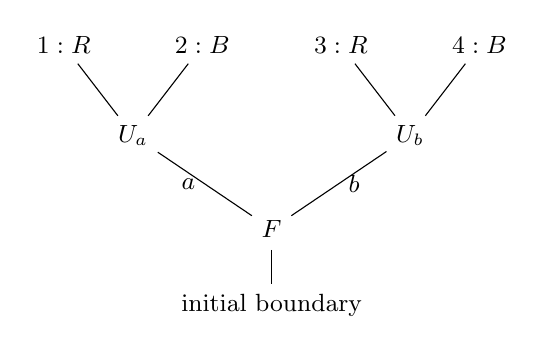
\begin{tikzpicture}[scale=.88,every node/.style={font=\small}]
 \node (F) at (0,0) {$F$};
 \node (A) at (-2,1.35) {$U_a$};
 \node (B) at (2,1.35) {$U_b$};
 \node (r1) at (-3,2.65) {$1:R$};
 \node (b2) at (-1,2.65) {$2:B$};
 \node (r3) at (1,2.65) {$3:R$};
 \node (b4) at (3,2.65) {$4:B$};
 \draw (F)--node[left]{$a$}(A);
 \draw (F)--node[right]{$b$}(B);
 \draw (A)--(r1) (A)--(b2) (B)--(r3) (B)--(b4);
 \draw (0,-.3)--(0,-.8);
 \node at (0,-1.1) {initial boundary};
\end{tikzpicture}
\caption{The four-tip body.  At a vertex where red ports are selected,
each upper torus can be compressed using its red cap; at the other
vertex of the double cover, both compressions use blue caps.}
\label{ch:grope-figure}
\end{figure}

Put $\mathcal C=\{1,l_1,\ldots,l_p\}$.  Install one body for every
ordered quadruple $(i_1,i_2,i_3,i_4)$ of distinct ports with colors
$(R,B,R,B)$, every independent choice $c_\alpha\in\mathcal C$, and
every independent sign $\varepsilon_\alpha\in\{1,-1\}$.  Its based
tips must represent
\begin{equation}
\label{ch:tip-markings}
 X_\alpha=c_\alpha x_{i_\alpha}^{\varepsilon_\alpha}c_\alpha^{-1},
 \qquad 1\leq\alpha\leq4,
\end{equation}
in the outside piece.  There are finitely many bodies; denote their
number by $k$, and use the same list in every translate of a block.

\begin{lemma}[The four-tip marked body]
\label{ch:four-tip-model}
The four-tip body has a three-dimensional handlebody thickening that,
with its four marked tip annuli, is a boundary connected sum of four
solid tori with longitudinal marked annuli.  The finite list above can
be placed with disjoint bodies and the markings
\eqref{ch:tip-markings} in the outside pieces of the plumbing.
The bottom surfaces are proper inward pushes of disjoint boundary
surfaces of $X$.  Each terminal cap is embedded and framed; it misses
all body sheets away from its own attachment.  The only possible
cap--cap intersections occur between opposite ports of a plumbing.
\end{lemma}

\begin{proof}
We extend the marked three-tip model of
\cite[Lemma~2.3]{MT}.  Thicken a punctured torus to its product with
an interval and put its two basis annuli on opposite faces.  Two
disjoint cutting arcs, each dual to one basis curve and disjoint from
the other, give disjoint meridian disks in the product.  To see these
arcs explicitly, puncture the square torus near $(1/2,1/2)$, take
the basis circles at $x=1/4$ and $y=1/4$, and cut along the arcs
at $y=1/2$ and $x=1/2$.  The puncture removes their only mutual
intersection.  Each product disk meets its own marked annulus in
one essential arc and misses the other.

Cutting the thickening along these disks gives a ball.  Each marked
annulus becomes a rectangle joining the two faces of its own cutting
disk.  The rectangle and those two disk faces have a disk neighbourhood
in the boundary sphere, disjoint from the analogous neighbourhood for
the other annulus.  A boundary homeomorphism, extended over the ball,
identifies this marked configuration with the standard one.  After
reattaching the handles, the lower thickening is therefore a boundary
connected sum of two longitudinal-annulus collars.  This is a statement
about the annuli themselves, not just their elements of the free group.

Attach an upper punctured-torus thickening along each of these two
annuli.  A longitudinal-annulus collar is a solid torus viewed as an
annulus times an interval; gluing it on merely collars the attaching
annulus of its upper thickening.  The single boundary-sum tube of the
lower model now joins the two upper thickenings.  Extend the two
meridian disks from each upper thickening through its own collar.
The feet of the joining tube can be chosen arbitrarily small in the
complement of the attaching annuli and moved away from the finitely
many extending disk strips.  The four extended disks are thus disjoint
and dual to the four tip annuli.  Cutting along them and repeating the
preceding ball argument proves the asserted four-tip marked model.
There is only one joining tube between the upper handlebodies, so no
additional free generator is introduced.  The initial boundary and
all the surface markings are transported with this identification.

For placement we use the refinement of
\cite[Section~2.2, ``The exterior with its side marking'']{PD}:
place the bodies in the complement of sufficiently thin attaching
solid tori in the initial one-handlebody boundary, and lengthen only
the returning tip collars to the attaching regions.  The connectors
and their basing paths then lie in $K_v$ after plumbing.  Reserve
separated product parallels of the attaching curves, one for each
occurrence of a tip, and join their thin longitudinal collars by
tubes along a rooted tree.  Let $\eta$ run from the outside basepoint
to its root and let $p_\alpha$ be the tree path from that root to
the $\alpha$th tip collar.  Choose these paths so that
$\eta p_\alpha$ is homotopic relative to its endpoints to
$c_\alpha\kappa_{i_\alpha}$, using the product tracks to identify
the parallel meridians.  Then
\[
 (\eta p_\alpha)m_{i_\alpha}^{\varepsilon_\alpha}
       (\eta p_\alpha)^{-1}
   =c_\alpha x_{i_\alpha}^{\varepsilon_\alpha}c_\alpha^{-1}
   \quad\text{in }\pi_1K_v.
\]
There is no compatibility restriction among the four chosen classes:
finitely many arcs in a three-manifold can realize them disjointly
away from their common root, with parallel tracks for repeated
portions and with the reserved returning strips avoided.  The tree
paths fix the required basing; other paths inside the resulting
handlebody add only words in its four tip generators.  The initial
boundaries remain in the outside pieces, and the bottom surfaces
are proper pushes of disjoint boundary surfaces of $X$.

We finally specify the framings.  The surface-product model frames a
surface by its oriented normal in the three-dimensional body and the
collar direction.  At a terminal annulus use the framing adjustment
in the proof of \cite[Lemma~2.3]{MT}, before fixing the returning
collar.  In a separated solid-torus neighbourhood this is the ribbon
twist
\[
 (\theta,z)\longmapsto(\theta,e^{in\theta}z).
\]
Replace $e^{in\theta}$, if necessary, by a smooth degree-$n$ circle map
$\phi(\theta)$ equal to $1$ near the connector feet.  The twist is
then the identity at those feet and extends by the identity over
the joining tubes.  Apply it to the complete marked body, including
the initial boundary and the lower and upper attaching annuli.

The returning collar is constructed after this transport.  In
coordinates $S^1_\theta\times D^2_z\times[0,1]_u$, choose an embedded
smooth regular plane arc $(r(s),u(s))$ from $(0,0)$ to $(0,1)$, departing in the
positive $r$ direction and vertical near its endpoint, with $u$
strictly increasing for $s>0$.  The collar
\[
 (\theta,s)\longmapsto
       (\theta,r(s)i\phi(\theta),u(s))
\]
leaves the transported surface ribbon in its outgoing normal
direction and ends at the same product circle $z=0,u=1$.  Its
normal quotient has frame
\[
 v=\phi(\theta),\qquad
 w=r'(s)\partial_u-u'(s)i\phi(\theta).
\]
At the first end this is the surface-transverse and collar frame;
at the last, up to a fixed constant change of frame, it has winding
$n$ relative to the core product frame.
Choose $n$ to match those framings.  The four disjoint longitudinal
neighbourhoods make the adjustments independent and leave the
external basing paths fixed.  The initial-boundary link and its
surface framing are fixed after these transports.  At each of the
three symplectic pairs, the attachments depart on opposite normal
sides.  Put the bodies at an inner collar level and extend the tips
into separated product parallels of the handle cores.  The collar
separation and the plumbing charts give the final assertions.
\end{proof}

We use the group commutator convention $[x,y]=xyx^{-1}y^{-1}$.

\begin{lemma}[The boundary laws]
\label{ch:laws}
For each installed body, its initial boundary represents, up to overall
conjugation, a word $L$ in the four based tips satisfying
\begin{equation}
\label{ch:law-properties}
 L\big|_{X_\alpha=1}=1\quad(1\leq\alpha\leq4),
 \qquad
 L\equiv [[X_1,X_2],[X_3,X_4]]
       \pmod{\Gamma_5 F(X_1,X_2,X_3,X_4)}.
\end{equation}
Here $\Gamma_r$ is the lower central series, and orientations are
chosen for the displayed sign.
\end{lemma}

\begin{proof}
The boundary of a punctured torus is the commutator of its based
symplectic generators.  Apply this first to the two upper tori and
then to the bottom torus.  Internal paths may conjugate a tip or an
upper commutator by words in the four tips.  Such conjugations change
the weight-four expression only in weight at least five.  If any
one tip is set equal to the identity, the commutator at its upper
torus becomes trivial, and then so does the bottom commutator.
These are word identities in the abstract tips; substituting the
markings \eqref{ch:tip-markings} gives the corresponding
initial-boundary words in $\pi_1K_v$.
\end{proof}

\subsection{The exterior and its homotopy type}

Write $F_1,\ldots,F_k$ for the bottom punctured tori, and $a_j,b_j$
for their two branch curves.  Both branch curves are null-homotopic
in $X$: an upper punctured torus and its terminal caps give a
null-homotopy.  Since $F_j$ retracts to its two branch curves and
$X$ has graph homotopy type, the entire map $F_j\to X$ is
null-homotopic.

Remove the interiors of disjoint product tubes of the $F_j$, including
their proper boundary collars, and put
\[
 E=X\setminus\bigcup_{j=1}^k\operatorname{int}\nu(F_j).
\]
The tubes can be chosen to avoid the upper caps and meet the upper
surfaces only along short attaching collars.  The exterior is
connected, since paths can be moved off the proper codimension-two
surfaces and then off sufficiently thin tubes.

The surface-product trivializations specify the following input from
\cite[Lemma~2.2]{PD}.

\begin{lemma}[The marked exterior model]
\label{ch:exterior-model}
There is a homotopy-pushout model
\begin{equation}
\label{ch:exterior-pushout}
 E\simeq X\cup_{\coprod_jF_j}\coprod_j(F_j\times S^1),
\end{equation}
where $F_j$ maps to $F_j\times S^1$ by its inward section.  Under
this model the displayed maps from $F_j\times S^1$ are the actual
tube-side maps, and $S^1$ is the normal circle.
\end{lemma}

The marking of the side maps is essential here.  The hypotheses of
the cited lemma hold because Lemma~\ref{ch:four-tip-model} places
the $F_j$ as proper pushes of disjoint boundary surfaces with their
surface-product trivializations.  The model can be seen in a boundary
collar: the outer part of the exterior contributes a bridge across
the deleted surface, while its inward normal semicircle supplies a
specified return path in the inner $X$ piece.  The bridge followed
by that return is exactly the tube's normal circle.  This identifies
the section and side maps in \eqref{ch:exterior-pushout}, as required
for the following gluing.

For each $j$, regard a solid torus $V_j$ as a compression body from
$F_j$ to a disk, compressing $a_j$.  Define
\begin{equation}
\label{ch:chamber-definition}
 D=E\cup_{\coprod_j(F_j\times S^1)}
             \coprod_j(V_j\times S^1),\qquad S=\partial D,
\end{equation}
using the product framings and rounding corners.  The remaining disk
face of $V_j$ contributes a solid torus to $S$.  Hence $S$ is the
surface-framed surgery of $\partial X$ along the initial-boundary
link.  In particular, $S$ is connected.

\begin{proposition}[The chamber homotopy type]
\label{ch:homotopy-type}
With the markings induced by the preceding construction,
\begin{equation}
\label{ch:group-and-spheres}
 H:=\pi_1D=\pi_1X*F(z_1,\ldots,z_k),\qquad
 D\simeq BH\vee\bigvee^{2k}S^2,
\end{equation}
where $BH$ is a finite graph and $z_j$ is the normal-circle generator
of the $j$th replacement.  On the common surgery-link exterior in
the boundary, killing the $z_j$ recovers the original marking into
$\pi_1X$.
\end{proposition}

\begin{proof}
The side-marked model of Lemma~\ref{ch:exterior-model} gives
\[
 D\simeq X\cup_{\coprod_jF_j}\coprod_j(V_j\times S^1).
\]
Because each attaching map $F_j\to X$ is null-homotopic, the
additional based summand is the homotopy cofiber of
$F_j\to V_j\times S^1$.  Retract $V_j\times S^1$ to the torus
on its longitude $b_j$ and normal circle $z_j$.  Since $F_j$
retracts to $a_j\vee b_j$, its cone adds one two-cell on the
trivial loop $a_j$ and another killing $b_j$.  Cancel the latter
one/two-cell pair.  The old torus two-cell, originally attached
by $[b_j,z_j]$, now has trivial attaching map.  The cofiber is
therefore
\[
 S^1_{z_j}\vee S^2\vee S^2.
\]
This proves \eqref{ch:group-and-spheres}.  The model retains the
normal-circle marking, so its quotient killing the new generators
is the old $X$-marking.  Equivalently, the classifying map to the
graph of $X$ extends over each replacement, since both $a_j$ and
$b_j$ map trivially and the new normal circle is sent to the
identity.  Its restriction to the common boundary exterior is the
original classifying map.
\end{proof}

\subsection{The middle form and the Poincar\'e chamber}

We next identify the entire middle homotopy module by framed
hyperbolic pairs.  This serves two purposes: it produces the
graph-type Poincar\'e pair required for reflection, and it makes
the double-cover filling an explicit geometric operation.
All intersection pairings below use fixed whiskers and the
involution $h\mapsto h^{-1}$ on the group ring.

Compress either upper punctured torus along either one of its
terminal caps.  Cutting the torus along that basis curve gives a
pair of pants, whose two new boundary curves are filled by opposite
parallel copies of the selected cap.  The result is an embedded
framed disk along the corresponding bottom branch, subject only
to intersections with other selected cap sheets.  The unused cap
does not belong to this disk.  The outgoing collar and its framing
are the local compression model of \cite[Lemma~2.4]{MT}.  At the
bottom torus the two upper attachments use distinct normal angles,
so this construction applies simultaneously on the $a_j$- and
$b_j$-branches.

\begin{lemma}[Algebraic duals]
\label{ch:exterior-duals}
There are proper framed immersed disks $f_j$ in $E$, bounded by
the truncated $a_j$-branch curves, and framed spheres $g_j$ in $E$
such that
\begin{equation}
\label{ch:dual-pairings}
 \lambda(f_i,g_j)=\delta_{ij},\qquad
 \lambda(g_i,g_j)=0
 \quad\text{over }\mathbb Z[\pi_1E].
\end{equation}
Each $g_j$ is embedded with trivial normal bundle.  If all terminal
caps selected for the branch compressions are mutually disjoint,
these representatives have exactly one geometric intersection
between $f_j$ and $g_j$ and no other intersections.
\end{lemma}

\begin{proof}
Choose one terminal cap on each upper torus.  Let $f_j$ be the
proper truncation of the compression disk on the $a_j$-branch, and
let $C_j$ be the compression disk on the $b_j$-branch.  Near the
tube side over $b_j$, take the normal-circle torus and compress it
with two parallels of $C_j$.  Denote the resulting sphere by $g_j$.

Here is the local collar calculation, from
\cite[Lemma~2.4]{MT}, that also checks its applicability to the
new $a_j$-branch.  Use coordinates $(s,t,r,\theta)$, where $s$
runs along $b_j$, $t$ is transverse to $b_j$ in $F_j$, and
$(r,\theta)$ are polar coordinates normal to $F_j$.  The rim
torus is $t=0$, $r=\rho$.  The outgoing $a_j$-disk collar and
the $b_j$-upper attachment have distinct angles
$\theta_A,\theta_B$.  Cut the rim torus at a narrow band around
$\theta_B$ and keep the annulus containing $\theta_A$.  Place
the interiors of its two compression disks outside $r=\rho$.
The retained annulus meets the $a_j$-disk collar once.  Orient
and base this point to contribute $1$.  This calculation only
uses the outgoing framed collar of that disk, so it remains
valid when the disk itself is obtained by upper-torus compression.
The disjoint body neighbourhoods exclude collar intersections
between different indices.

Every remaining intersection occurs in a cap--cap plumbing chart.
Within $g_j$, label the two copies of $C_j$ by
$\epsilon\in\{+1,-1\}$ and the two cap sheets in a fixed copy
by $\eta\in\{+1,-1\}$.  Their orientation coefficients are
$\epsilon\eta$.  Fix $\epsilon$ and an opposing sheet.  The
whisker on the opposing sheet is held fixed in this comparison.
The two paths on $g_j$ share the whole stem from the rim to the
fixed copy of $C_j$ and split only inside its upper torus.  Their
difference there is the other basis loop, which bounds the
unused terminal cap in $E$: no upper cap was removed with the
bottom tubes.  A small normal turn around the upper surface
also bounds in $E$, because that surface has not been deleted.
The two intersection labels are consequently the same element
$h\in\pi_1E$, and their contributions cancel as
\[
 \epsilon\eta h+\epsilon(-\eta)h=0.
\]
Figure~\ref{ch:sheet-cancellation} displays the two cancellations.
The outer index $\epsilon$ is fixed throughout this cancellation;
we make no identification of paths that differ by a bottom
normal circle.  The opposing sheet may come either from another
rim sphere or from the compressed $a$-branch.  This proves
\eqref{ch:dual-pairings}.

\begin{figure}[ht]
\centering
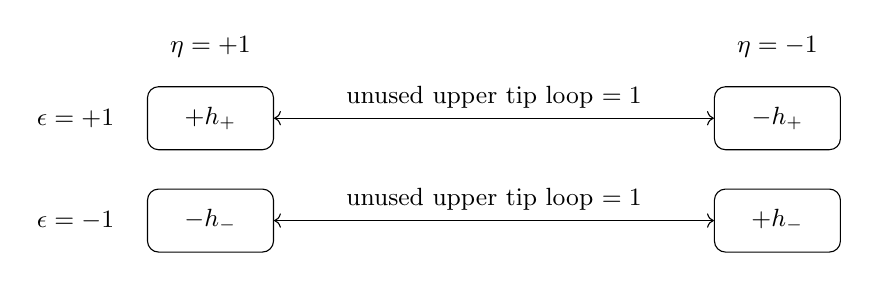
\begin{tikzpicture}[x=1cm,y=1cm,every node/.style={font=\small},
 contribution/.style={draw,rounded corners,minimum width=16mm,minimum height=8mm}]
 \node at (0,2.2) {$\eta=+1$};
 \node at (7.2,2.2) {$\eta=-1$};
 \node[anchor=east] at (-1.1,1.3) {$\epsilon=+1$};
 \node[anchor=east] at (-1.1,0) {$\epsilon=-1$};
 \node[contribution] (pp) at (0,1.3) {$+h_+$};
 \node[contribution] (pm) at (7.2,1.3) {$-h_+$};
 \node[contribution] (mp) at (0,0) {$-h_-$};
 \node[contribution] (mm) at (7.2,0) {$+h_-$};
 \draw[<->] (pp)--node[above]{unused upper tip loop $=1$}(pm);
 \draw[<->] (mp)--node[above]{unused upper tip loop $=1$}(mm);
\end{tikzpicture}
\caption{The four cap-sheet contributions in $g_j$, for one fixed
opposing sheet and up to its common intersection sign.  Rows index
the outer parallel copies of $C_j$ by $\epsilon$; columns index the
inner cap parallels by $\eta$.  The unused cap identifies the two
group labels within each row, so that row cancels.  No comparison
between $h_+$ and $h_-$ is made: the paths for different rows can
differ by a bottom normal circle.  This is a diagram of contributions,
not a projection of embedded surfaces, following the sheet calculation
in \cite[Lemma~2.4]{MT}.}
\label{ch:sheet-cancellation}
\end{figure}

A rim sphere uses only parallel copies of a single selected
terminal cap.  That core has no self-plumbing.  The separated
collars therefore make each sphere embedded, and the product
compression framings give its trivial normal bundle.  If the
selected caps are all disjoint, there are no plumbing
intersections at all; the single collar intersection in each
pair is then the complete geometric intersection set.
\end{proof}

Close $f_j$ by the meridian disk of $V_j$ at its fixed normal-circle
coordinate, obtaining a sphere $u_j\subset D$.  The framings agree:
on the $f_j$ side the frame is transverse to $a_j$ inside $F_j$
together with the circle direction, while on the meridian-disk
side it extends as the solid-torus transverse direction and the
product-circle direction.  Thus $u_j$ is framed.  Lemma~\ref{ch:exterior-duals}
gives
\begin{equation}
\label{ch:middle-pairings}
 \lambda(u_i,g_j)=\delta_{ij},\qquad
 \lambda(g_i,g_j)=0
 \quad\text{over }\Lambda:=\mathbb ZH.
\end{equation}

\begin{proposition}[The Poincar\'e chamber]
\label{ch:poincare-chamber}
The manifold $D$ has a specified framed immersed hyperbolic basis
for its full module $\pi_2D$, with vanishing quadratic
self-intersections.  Attach one three-cell on each of these
$2k$ basis spheres, and call the resulting space $P$.  Then
$(P,S)$ is an oriented finite four-dimensional Poincar\'e pair,
the inclusion $(D,S)\to(P,S)$ preserves the fundamental group
and the boundary, and $P\simeq BH$.
\end{proposition}

\begin{proof}
We give the middle-form verification used in
\cite[Section~2.3, ``The middle form and the Poincar\'e pair'']{PD}.
The hermitian matrix of the $u_i$ has even identity coefficient
on its diagonal, since their normal framings give zero
Stiefel--Whitney evaluations.  The free group $H$ has no
nonidentity element of order two.  Hence each diagonal entry
can be written $z+\overline z$: choose one coefficient from
each nonidentity inverse pair and halve the even identity
coefficient.  Subtracting suitable $\Lambda$-linear combinations
of the $g_j$ from the $u_i$, using a triangular half off the
diagonal and these halves on the diagonal, makes all pairings
among the modified $u_i$ vanish.  The cross-pairings and the
$g_i,g_j$ pairings in \eqref{ch:middle-pairings} are unchanged.

Represent these classes by immersed spheres using the usual
tubing operations.  Their even normal parity permits framed
representatives.  Write $\mu$ for the full framed Wall invariant
in the additive quotient
\[
 \Lambda/\langle h-h^{-1}:h\in H\rangle_{\mathbb Z};
\]
in particular, its identity coefficient is retained.  For a framed
representative, the symmetrization identity
\[
 \lambda(v,v)=\mu(v)+\overline{\mu(v)}
\]
and the absence of order-two elements show that its Wall
quadratic self-intersection is zero when its self-pairing
vanishes.  This is the framed immersed-sphere calculation in
the cited section; no embedded-surgery theorem is used.
Write $A_j,B_j$ for the resulting hyperbolic pairs.

They form a basis of the whole module.  By
Proposition~\ref{ch:homotopy-type}, $\pi_2D$ is free of rank
$2k$ over $\Lambda$.  Relative to any such basis, the square
matrix with columns $A_j,B_j$ has a left inverse supplied by
its nonsingular hyperbolic pairing.  Matrix rings over
$\mathbb ZH$ are directly finite: pass a one-sided inverse
identity to every finite quotient of $H$, use the finite
dimensional regular representation over $\mathbb C$ to obtain
the reverse identity, and then use residual finiteness to
separate the finite support of any nonzero group-ring entry.
The matrix therefore has a two-sided inverse.

A map from $BH\vee\bigvee^{2k}S^2$ to $D$ realizing this
basis is a homotopy equivalence: it induces the marked
isomorphism on $\pi_1$ and an isomorphism on the homology of
the simply connected covers.  Attaching the indicated
three-cells cancels the sphere summands in that homotopy
type.  Thus $P\simeq BH$.

For completeness, the duality argument of \cite[Section~2.3]{PD}
applies to exactly this basis.  The middle sphere module of
$D$ maps isomorphically to a split summand of
$H_2(D,S;\Lambda)$ by its nonsingular intersection form.
The three-cell attachments quotient the absolute and relative
middle homology by these summands; their attaching map is
injective on the summands, so no new third homology appears.
In cohomology the pullbacks identify the new groups with the
annihilators of the sphere summands.  If $i:(D,S)\to(P,S)$ is
the inclusion and $[P,S]=i_*[D,S]$, cap-product naturality
gives
\[
 \alpha\frown[P,S]
   =i_*\bigl(i^*\alpha\frown[D,S]\bigr).
\]
The duality isomorphisms for $(D,S)$ consequently induce
duality on these annihilators and quotients.  The finite
free chain complexes over $\Lambda$ give the regular-coefficient
criterion for Poincar\'e duality with all local coefficients.
This proves the assertion for $(P,S)$, with its original
boundary collar and orientation.
\end{proof}

\begin{corollary}[Connected lifted boundary]
\label{ch:boundary-surjectivity}
The boundary marking $\pi_1S\to H$ is surjective.
\end{corollary}

\begin{proof}
Duality for $(P,S)$ and the graph homotopy type of $P$ give
\[
 H_1(P,S;\mathbb ZH)=H_0(P,S;\mathbb ZH)=0.
\]
Therefore
$H_0(S;\mathbb ZH)\to H_0(P;\mathbb ZH)$ is an isomorphism.
The source is free abelian on the cosets of the image of
$\pi_1S$, whereas the target is $\mathbb Z$.  There is only
one coset.
\end{proof}

\subsection{Cyclic covers and marked fillings}
\label{ch:cyclic-covers}

Define the epimorphism
\begin{equation}
\label{ch:cover-character}
 w:H\longrightarrow\mathbb Z,\qquad
 w(\tau_r)=1,\quad w(l_s)=w(z_j)=0.
\end{equation}
For $d\geq1$, let
\[
 H_d=\ker(H\xrightarrow{w}\mathbb Z\longrightarrow\mathbb Z/d),
\]
and denote the associated connected covers by $D_d,P_d,S_d$.
We also write $X_d$ for the plumbing cover obtained by restricting
$w$ to $\pi_1X$.  The plumbing graph of $X_d$ has vertices
$\mathbb Z/d$, an edge of each type $r$ from $v$ to $v+1$,
and $p$ extra loops at every vertex.  Its bodies are copies of
the full marked list at each vertex.

\begin{lemma}[Persistence of the chamber data]
\label{ch:cover-data}
For every $d$, the data $(D_d,P_d,S_d,H_d)$ satisfy
Propositions~\ref{ch:homotopy-type} and~\ref{ch:poincare-chamber}
with all the bodies and basis spheres lifted.  In particular,
$S_d$ is connected, $H_d$ is free, $P_d\simeq BH_d$, and
$(P_d,S_d)$ is the oriented Poincar\'e pair obtained by
attaching three-cells to a specified framed immersed
hyperbolic basis of $D_d$.
\end{lemma}

\begin{proof}
Corollary~\ref{ch:boundary-surjectivity} gives connectedness
of $S_d$.  The side-marked exterior model identifies the
covering character on $\pi_1E$ with the one inherited from
$X$, with each normal circle sent to zero.  Its restriction
to $\pi_1(V_j\times S^1)$ is trivial: the longitude maps
trivially in $H$ and $w(z_j)=0$.  Thus the cover of each
replacement is trivial, and performing the chamber
construction on every lifted body in $X_d$ gives $D_d$.
The cofiber calculation is unchanged.

Each basis sphere has $d$ lifts.  Algebraically, the universal
cover is the same and its free middle module is restricted
from $\mathbb ZH$ to $\mathbb ZH_d$.  Pairings of two
chosen lifts are obtained by taking, in the pairing of their
corresponding coset translates, the coefficients supported
in $H_d$.  The lifted hyperbolic pairings are therefore standard.
The Wall invariant of a chosen lift is obtained, after the corresponding
change of whisker, by retaining precisely the self-intersection labels
in $H_d$.  Because $H_d$ is closed under inversion, this additive
coefficient projection retains the identity and both members of every
retained inverse pair.  It therefore descends to the framed Wall
quotient and carries the zero downstairs invariant to zero.
The lifted sphere classes are a basis of the
restricted module.  The three-cell attachments and the
orientation lift, giving the asserted pair.
\end{proof}

\begin{definition}[Marked filling]
\label{ch:marked-filling}
A marked filling of $S_d$ is a compact oriented topological
four-manifold $D'_d$, an orientation-preserving identification
$\partial D'_d=S_d$, and a homotopy equivalence
$D'_d\to BH_d$ whose boundary restriction is homotopic to
the marking $S_d\to P_d\simeq BH_d$.
\end{definition}

Such a filling also admits a homotopy equivalence
\begin{equation}
\label{ch:relative-filling-map}
 (D'_d,S_d)\longrightarrow(P_d,S_d)
\end{equation}
that is the identity on $S_d$.  Indeed, compose its marking
with a homotopy inverse $BH_d\to P_d$.  The boundary
restriction is homotopic to the prescribed inclusion;
the homotopy extension property of a boundary collar
changes the map to one equal to that inclusion, without
changing its homotopy-equivalence class.

\begin{proposition}[The double-cover filling]
\label{ch:even-filling}
The boundary $S_2$ has a marked filling $D'_2$.  It can be
obtained from $D_2$ by replacing disjoint punctured
$S^2\times S^2$ neighbourhoods by four-balls.  In particular,
there is a homotopy equivalence $(D'_2,S_2)\to(P_2,S_2)$
equal to the identity on the boundary.
\end{proposition}

\begin{proof}
At vertex $0$ of the plumbing double cover select all red
ports, and at vertex $1$ select all blue ports.  Every
plumbing edge joins these two vertices and has the same
color at both ends.  Exactly one end is selected.
Consequently all product cap parallels belonging to
selected ports are mutually disjoint.  This also accounts
for the two different lifts of each original plumbing
type: each has one selected end, independently of its
orientation in the two-vertex graph.

Each upper torus of each body has one red and one blue
tip.  Compress it using the cap selected at its vertex.
Use these choices on both upper branches to construct
$u_j,g_j$ in $D_2$, with $j$ now ranging over the lifted
bodies.  Lemma~\ref{ch:exterior-duals} and the matching
meridian-disk framings show that these are embedded framed
pairs with a single transverse intersection inside each
pair and no intersections between different pairs.
Their hyperbolic pairing and the known free rank show,
by the same direct-finiteness argument as in
Proposition~\ref{ch:poincare-chamber}, that their classes
form a basis of $\pi_2D_2$.

A regular neighbourhood $N_j$ of one such pair is the
normal plumbing of two trivial disk bundles over $S^2$
at one point.  This is the standard punctured
$S^2\times S^2$: take tubular neighbourhoods of the two
factor spheres in $S^2\times S^2$, whose rounded
complement is a ball.  Reversing one sphere orientation
if necessary matches the intersection sign.  Thus
$\partial N_j\cong S^3$.  Choose these neighbourhoods
disjointly in the interior of $D_2$, and set
\[
 A=\overline{D_2\setminus\bigcup_jN_j},\qquad
 D'_2=A\cup_{\coprod_j\partial N_j}\coprod_jB^4.
\]
The complement $A$ is connected: any segment of a path
through $N_j$ can be replaced by a path along its connected
boundary.  Since $N_j$, $\partial N_j$, and $B^4$ are
simply connected, van Kampen gives the same marked
fundamental group $H_2$ for $A$, $D_2$, and $D'_2$.

We verify contractibility of the universal cover of $D'_2$.
Write $\widetilde A$ for the common lifted complement.
The universal cover of $D_2$ is obtained by adjoining all
lifts of the $N_j$, whereas the universal cover of $D'_2$
is obtained by adjoining balls at the same boundary
spheres.  These are locally finite families, and their
homology contributions are direct sums.  In degree two,
Mayer--Vietoris gives
\[
 H_2(\widetilde A;\mathbb Z)\oplus
       \bigoplus_{\widetilde N_j}H_2(\widetilde N_j;\mathbb Z)
       \ \cong\ H_2(\widetilde D_2;\mathbb Z).
\]
The second summand maps isomorphically onto the right-hand
side because the lifted sphere pairs are a free middle
basis.  Hence $H_2(\widetilde A;\mathbb Z)=0$.
Since $\widetilde D_2$ has the homotopy type of a wedge of
two-spheres, the same exact sequence in the adjacent
degrees gives
\[
 H_4(\widetilde A;\mathbb Z)=0,\qquad
 \bigoplus_{\widetilde N_j}H_3(\partial\widetilde N_j;\mathbb Z)
      \xrightarrow{\ \cong\ }H_3(\widetilde A;\mathbb Z).
\]
Adjoining the balls kills exactly these third-homology
classes and produces no fourth homology.  It leaves the
zero second homology unchanged.  The resulting cover is
simply connected, and its reduced homology vanishes in
every degree.  Manifolds have CW homotopy type, so the
homological Whitehead theorem makes this cover
contractible.  Therefore $D'_2\simeq BH_2$.

All modifications were interior, and the fundamental-group
identifications above agree on $S_2$.  A classifying map
$D'_2\to BH_2$ consequently has the prescribed boundary
marking, since maps to $BH_2$ are determined up to homotopy
by that group marking.  This is the required marked
filling, and \eqref{ch:relative-filling-map} gives the
relative homotopy equivalence to $P_2$.
\end{proof}

The remaining task for the chamber is the converse parity
phenomenon: for every odd $d\geq3$, no marked filling of
$S_d$ exists.  Its proof uses all the boundary laws from
Lemma~\ref{ch:laws}; the color choice used above explains
why the corresponding obstruction must distinguish odd
cycles from the two-vertex cover.

\section{A tensor obstruction on a graph}\label{sec:tensors}

The obstruction needed here is governed by the plumbing graph associated
to a hypothetical marked filling.  We prove that formal data on the
corresponding cut pieces force an assignment of every edge to one endpoint
such that, at each vertex, no prescribed set of incident edges is assigned
entirely to that vertex.  On the colored odd cycle used in the construction,
no such assignment exists.  The truncated differential forms and the two
successive homologies in the proof come from the finite tensor obstruction of
\cite[Section~3]{MT}.  We give the algebraic argument in full, including the
passage from two vertices to an arbitrary graph.

\subsection{The incidence theorem}

Let \(\Gamma=(V,E)\) be a finite multigraph without loops.  Distinguish its
two endpoints as \(v_+(e)\) and \(v_-(e)\) for every \(e\in E\).  Write
\(E_+(v)\), \(E_-(v)\), and \(E(v)\) for the edges having plus endpoint
\(v\), minus endpoint \(v\), and either endpoint \(v\), respectively.
An endpoint assignment is a function \(a:E\to V\) with
\(a(e)\in\{v_+(e),v_-(e)\}\).

For a field \(K\), denote by \(K\langle h\rangle\) the ring of algebraic
power series, viewed as the henselization of \(K[h]_{(h)}\) inside
\(K[[h]]\).  Thus its elements have finite pointed \(\acute{e}\)tale
presentations.  All derivatives below act on internal coordinates; the
parameters \(t_e\) are held fixed.  Empty products are equal to one, and a
coordinate block is allowed to have dimension zero.

\begin{theorem}[Endpoint assignment]\label{ten:assignment}
Let \(K\) have characteristic zero, and let \(\Gamma\) be a finite
loopless multigraph with distinguished endpoints as above.  For each edge
\(e\), choose a coordinate block \(h_e\) of dimension \(N_e\geq0\) and
functions \(F_e,b_e\in K\langle h_e\rangle\).  For each vertex \(v\),
choose a family \(\mathcal L_v\) of nonempty subsets of \(E(v)\), and set
\begin{align}
 T_v&=K[t_e:e\in E_+(v)]/(t_e^2:e\in E_+(v)),\label{ten:parameters}\\
 \mathcal S_v(h,t)
 &=\sum_{e\in E_+(v)}(F_e(h_e)+t_e b_e(h_e))
       -\sum_{e\in E_-(v)}F_e(h_e).\label{ten:vertex-potential}
\end{align}
Suppose there are formal parametrizations
\[
 M_v(y_v,t)\in (y_v,t)T_v[[y_v]]^{\sum_{e\in E(v)}N_e},
 \qquad y_v=(y_{v,1},\ldots,y_{v,a_v}),
\]
satisfying the following conditions.
\begin{enumerate}
 \item The central tangent maps \(A_v=\partial_{y_v}M_v(0,0)\) are
 injective, and the difference map
 \begin{equation}\label{ten:transversality}
 \begin{split}
 \Lambda:\bigoplus_{v\in V}K^{a_v}&\longrightarrow
                         \bigoplus_{e\in E}K^{N_e},\\
 (\xi_v)_v&\longmapsto
 \bigl((A_{v_+(e)}\xi_{v_+(e)})_e
             -(A_{v_-(e)}\xi_{v_-(e)})_e\bigr)_e
 \end{split}
 \end{equation}
 is an isomorphism.
 \item One has \(\mathcal S_v(M_v(y_v,t),t)=0\) identically for every
 vertex \(v\).
 \item For every \(L\in\mathcal L_v\), put
 \(I=L\cap E_+(v)\) and \(J=L\cap E_-(v)\).  Then
 \begin{equation}\label{ten:law-membership}
 \left(\prod_{i\in I}t_i\right)
 \left(\prod_{j\in J}b_j\right)(M_v)
 \in
 \bigl((\partial_h\mathcal S_v)(M_v)\bigr)
                         \subset T_v[[y_v]].
 \end{equation}
 The ideal on the right is generated by all restricted internal
 partial derivatives of \(\mathcal S_v\).
\end{enumerate}
There is an endpoint assignment \(a:E\to V\) such that, for every
\(v\in V\) and \(L\in\mathcal L_v\), at least one edge of \(L\) is
assigned to its endpoint other than \(v\).
\end{theorem}

Injectivity in the first condition makes every parametrization a smooth
formal graph, also over the full parameter ring \(T_v\).  In particular,
nilpotent constant displacements are permitted.  The relations in
\eqref{ten:parameters} are individual relations: products of distinct
parameters remain present.

Before proving the theorem, we record its consequence for the graph used
in the chamber construction.

\begin{corollary}[Colored odd cycles]\label{ten:odd-cycle}
Let \(d\geq3\) be odd.  On the cycle with vertices \(\mathbb Z/d\mathbb Z\),
replace every neighboring pair by five red and five blue parallel
edges.  Distinguish the two endpoints of each edge arbitrarily.  At
each vertex let \(\mathcal L_v\) consist of every four-element subset
of incident edges containing two red and two blue edges.  There are
no data satisfying the hypotheses of Theorem~\ref{ten:assignment} for
this graph and these law families.
\end{corollary}

\begin{proof}
An assignment supplied by Theorem~\ref{ten:assignment} cannot assign
two red and two blue edges to the same vertex.  Hence every vertex
receives at most one edge in at least one of the two colors.
Call such a color deficient at that vertex.  Two adjacent vertices
cannot share a deficient color: each of the five edges of that color
joining them must be assigned to one of the two vertices, whereas together
the two vertices could receive at most two.  Thus the nonempty sets of
deficient colors at adjacent vertices are disjoint.  Each such set
is consequently a singleton, and the deficient colors alternate
around the cycle.  This is impossible when \(d\) is odd; see
Figure~\ref{ten:cycle-figure}.
\end{proof}

\begin{figure}[hbp]
\centering
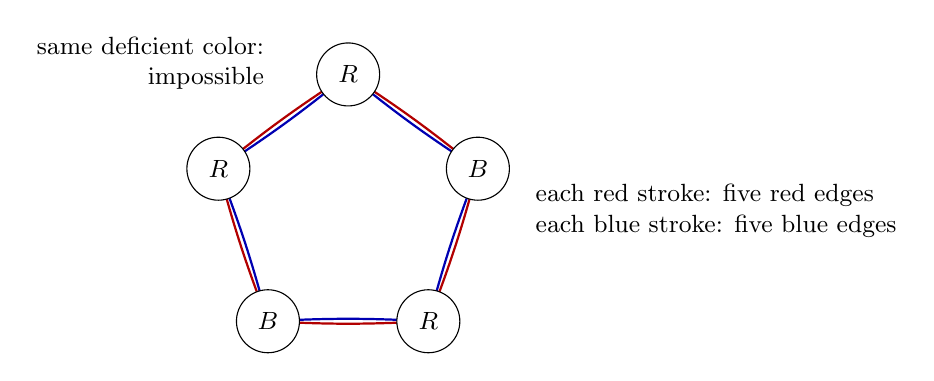
\begin{tikzpicture}[scale=1.05,
  deficiency/.style={circle,draw,fill=white,minimum size=8mm,inner sep=0pt},
  every node/.style={font=\small}]
 \coordinate (v0) at (90:1.65);
 \coordinate (v1) at (18:1.65);
 \coordinate (v2) at (-54:1.65);
 \coordinate (v3) at (-126:1.65);
 \coordinate (v4) at (162:1.65);
 \foreach \i/\j in {0/1,1/2,2/3,3/4,4/0}{
  \draw[red!70!black,line width=0.8pt]
    (v\i) to[bend left=3] (v\j);
  \draw[blue!70!black,line width=0.8pt]
    (v\i) to[bend right=3] (v\j);
 }
 \node[deficiency] at (v0) {\(R\)};
 \node[deficiency] at (v1) {\(B\)};
 \node[deficiency] at (v2) {\(R\)};
 \node[deficiency] at (v3) {\(B\)};
 \node[deficiency] at (v4) {\(R\)};
 \node[anchor=south east,align=right] at (-0.9,1.35)
    {same deficient color:\\impossible};
 \node[anchor=west,align=left] at (2.15,0)
    {each red stroke: five red edges\\
     each blue stroke: five blue edges};
\end{tikzpicture}
\caption{The deficient-color contradiction on a five-cycle.
Letters denote colors in which the vertex receives at most one edge.
Adjacent vertices must have different letters, so the forced alternation
fails when the cycle closes.}\label{ten:cycle-figure}
\end{figure}

For the application, a hypothetical filling is cut into vertex pieces
meeting along three-dimensional edge cuts.  Section~\ref{sec:formal}
constructs the functions \(F_e,b_e\) and graphs \(M_v\) from connection
data on these pieces.  The three hypotheses arise from transversality,
cancellation of boundary actions, and disk-bounding marked laws; the
gradient ideals encode flatness in the chosen formal families.

It remains to prove Theorem~\ref{ten:assignment}.  The proof converts
the vertex graphs into tensors whose contraction along
all edges is nonzero.  The law memberships force certain coefficients of
these tensors to vanish.  A nonzero term of the contraction then chooses
the required endpoint for every edge.  The argument uses the given graph
directly; it does not require a bipartition.

\subsection{Reduction to a finite-dimensional setting}

\begin{lemma}[Finite specialization]\label{ten:specialization}
If data satisfying the hypotheses of Theorem~\ref{ten:assignment} exist,
the same algebraic identities, ideal memberships, and tangent conditions
can be realized over a finite field of characteristic \(q\), for arbitrarily
large primes \(q\), with the same graph and law families.  The functions
\(F_e,b_e\) remain algebraic and depend only on their own edge block.
\end{lemma}

\begin{proof}
At each vertex choose a linear projection of the ambient coordinate space
onto \(K^{a_v}\) that is invertible on the central tangent image.
Its composite with \(M_v\) has a formal inverse over \(T_v\), with
parameters fixed.  The possible constant displacement lies in the
nilpotent ideal \((t)\), so the substitution is well defined.  Reparametrize
to make this projection of \(M_v\) equal to \(y_v\).

For a subset \(A\subset E_+(v)\), write \(t_A=\prod_{e\in A}t_e\).
Expand the graph and every coefficient witnessing
\eqref{ten:law-membership} in the finite basis \(\{t_A\}_A\) of \(T_v\).
All the resulting unknown coefficient series have the same independent
variables \(y_v\).  Represent the fixed edge functions on pointed
\(\acute{e}\)tale neighborhoods.  Implicit differentiation expresses their
ambient derivatives in the same finite presentations, with inverse
Jacobian determinants included among the units.  Auxiliary variables for
these presentations and units turn the following requirements into a
finite polynomial system in the unknown coefficient series:
the presentation equations, the fixed graph projection, the vanishing of
\(\mathcal S_v\), and all the ideal-membership identities.  No derivative
of an unknown coefficient series occurs.

Artin approximation over \(K[y_v]_{(y_v)}^h\)
\cite[Theorem~1.10]{Artin1969} gives algebraic coefficient series that
still solve this polynomial system exactly and agree with the original
solution through first order.  In particular, the central graph tangent
and all chosen branch centers are preserved.
Apply it separately at each vertex.  These systems share only the fixed
edge functions, and their mutual transversality is a condition on the
preserved first jets.  Thus no nested approximation is involved.  When
\(a_v=0\), the coefficient system already consists of equations over
\(K\), and no approximation is needed there.
The preserved branch centers and invertible Jacobians identify the
auxiliary solutions uniquely with the compositions of the fixed edge
germs and the approximated graph.

We now have finitely many algebraic germs and exact identities between
them.  Each is represented at a finite stage of a henselization, and every
identity holds at a sufficiently large finite stage.  Descend these
presentations, compositions, branch centers, and identities to a finitely
generated integral \(\mathbb Z\)-subalgebra \(A\subset K\).  Include the
inverse \(\acute{e}\)tale Jacobians and the inverse determinant in
\eqref{ten:transversality}.  The implicit differentiation identities
descend as well, so specialization preserves the meaning of the gradient
entries.  The original presentations for \(F_e,b_e\) still use only
\(h_e\).

There are specializations of \(A\) to finite fields in arbitrarily large
characteristic.  Indeed, a maximal quotient of the nonzero finite-type
\(\mathbb Q\)-algebra \(A\otimes\mathbb Q\) is a number field \(E_0\).
The images of a finite set of generators of \(A\), including all the
specified inverses, lie in \(\mathcal O_{E_0}[1/d_0]\) for some positive
integer \(d_0\).  Reduction at a prime above any rational prime not
dividing \(d_0\) gives the desired specialization.  All declared units
remain invertible.  The pointed \(\acute{e}\)tale presentations therefore
give formal germs satisfying the same identities and tangent conditions
over the residue field.
\end{proof}

Fix such a field \(k\) of characteristic \(q>2\).  For each edge define
\[
 R_e=k[h_{e,1},\ldots,h_{e,N_e}]/
                    (h_{e,1}^q,\ldots,h_{e,N_e}^q),
 \qquad
 \Omega_e=R_e\otimes_k
             \bigwedge\langle \mathrm dh_{e,1},\ldots,
                                      \mathrm dh_{e,N_e}\rangle .
\]
Let \(\mathrm d\) denote the exterior differential.  It is well defined
because \(\mathrm d(h_{e,r}^q)=0\).  We always use the graded tensor
convention: moving homogeneous factors of exterior degrees \(r,s\) past
one another contributes \((-1)^{rs}\).

Order the coordinates in each block and define integration to be zero
outside exterior degree \(N_e\), and otherwise to extract the coefficient
of \(\prod_r h_{e,r}^{q-1}\) from the coefficient of
\(\mathrm dh_{e,1}\wedge\cdots\wedge\mathrm dh_{e,N_e}\).
For a zero-dimensional block, this is the identity on \(k\).  Integration
kills exact forms, since differentiating a monomial cannot produce
exponent \(q-1\) in the differentiated coordinate.  Thus
\begin{equation}\label{ten:integration-parts}
 \int\mathrm d\alpha\wedge\beta
       =-(-1)^{|\alpha|}\int\alpha\wedge\mathrm d\beta
\end{equation}
for homogeneous forms.

These constructions extend to products of edge blocks and to the
square-free parameter rings by tensoring and differentiating only the
internal coordinates.  They turn the formal graphs into finite tensors
without discarding any of the parameter coefficients needed by the laws.

The projection normalization in Lemma~\ref{ten:specialization} also
provides explicit graph equations.  Complete its projected coordinates
\(x\) to linear ambient coordinates \((x,z)\).  The graph is then
\((x,f(x,t))\), and its equations are \(c_s=z_s-f_s(x,t)\).
We use these equations for the vertex graphs in the next construction.

\begin{lemma}[Graph forms]\label{ten:graph-forms}
Let \(c_1,\ldots,c_r\) be graph equations for a smooth formal graph over
one of the square-free parameter rings, centered modulo its parameter
ideal.  In the truncated differential forms of its ambient space, set
\begin{equation}\label{ten:graph-form}
 U_c=\bigwedge_{s=1}^r c_s^{q-1}\mathrm dc_s.
\end{equation}
Then \(\mathrm dU_c=0\); the graph ideal annihilates \(U_c\); and every
internal one-form restricting to zero on the graph wedges to zero with
\(U_c\).
\end{lemma}

\begin{proof}
Every centered-modulo-parameters series \(c\) has \(c^q=0\) in the
truncated ring.  By Frobenius, a nonconstant internal monomial acquires
an exponent at least \(q\), and a positive parameter monomial has zero
\(q\)-th power.  Consequently every formal coordinate change with such
a center preserves the truncation ideal; its inverse proves equality of
the ideals.  This also justifies evaluating the formal series in the
truncated ring.

Each factor \(c_s^{q-1}\mathrm dc_s\) is closed, and multiplication by
\(c_s\) kills it.  In graph coordinates, a one-form vanishing on the graph
is a sum of graph-ideal multiples of one-forms and multiples of the
\(\mathrm dc_s\).  Both types wedge to zero with \(U_c\).  The coordinate
invariance just proved permits this calculation after truncation and
over the full parameter ring.
\end{proof}

Choose a graph form \(U_{v,t}\) for each \(M_v\), and let
\[
 D_{v,t}=\mathrm d\mathcal S_v\wedge(-).
\]
The exact graph identity gives \(D_{v,t}U_{v,t}=0\).
The law memberships have a useful stronger consequence at the level of
actual forms:
\begin{equation}\label{ten:law-boundary}
 \left(\prod_{i\in I}t_i\right)
 \left(\prod_{j\in J}b_j\right)U_{v,t}
                         \in\operatorname{im}D_{v,t}.
\end{equation}
To see this, lift each membership coefficient from the graph to its
ambient coordinates.  The error in the resulting scalar identity is in
the graph ideal and hence kills \(U_{v,t}\).  If \(\iota_r\) is contraction
with an ambient coordinate vector, then
\[
 \iota_rD_{v,t}+D_{v,t}\iota_r
             =(\partial_{h_r}\mathcal S_v)\operatorname{id}.
\]
Applying this identity to the cycle \(U_{v,t}\) writes the scalar multiple
as a boundary.  The operator \(D_{v,t}\) is multiplication by a one-form
and does not differentiate the membership coefficients.  In particular,
\eqref{ten:law-boundary} survives every parameter specialization as an
equation on forms; no assertion about homology base change is needed.

\subsection{Two homologies and a nonzero contraction}

At each edge set
\begin{equation}\label{ten:edge-homologies}
 D_e=\mathrm dF_e\wedge(-),\qquad
 \mathcal H_e=H(\Omega_e,D_e),\qquad
 \delta_e=[\mathrm d],\qquad
 \mathcal W_e=H(\mathcal H_e,\delta_e).
\end{equation}
Here \(\delta_e\) is well defined because
\(\mathrm dD_e+D_e\mathrm d=0\).  The two homologies serve different
purposes: \(D_e\)-boundaries encode the gradient memberships, while
\(\delta_e\)-cycles supply the parameter lifts used below.

The wedge pairing followed by integration is perfect on \(\Omega_e\),
pairing complementary exterior degrees.  This follows directly by
pairing complementary monomials and complementary exterior basis
elements.  For any one-form \(\theta\),
\begin{equation}\label{ten:wedge-adjoint}
 (\theta\wedge\alpha)\wedge\beta
           =(-1)^{|\alpha|}\alpha\wedge(\theta\wedge\beta).
\end{equation}
Thus the annihilator of the \(D_e\)-cycles is exactly the space of
\(D_e\)-boundaries: one inclusion follows from
\eqref{ten:wedge-adjoint}, and equality follows from the equality of the
ranks of an operator and its adjoint.  The pairing descends to a perfect
pairing on \(\mathcal H_e\).  Equation~\eqref{ten:integration-parts}
gives the same argument for \(\delta_e\), and hence a perfect pairing on
\(\mathcal W_e\).  Replacing \(D_e\) by \(-D_e\) changes neither its
cycles nor its boundaries.

For clarity, the K\"unneth identifications used here are purely
finite-dimensional linear algebra.  Any finite-dimensional complex over
a field splits as its homology representatives with zero differential
and a direct sum of contractible two-term complexes.  A tensor product
with a contractible factor is contractible, using its contracting
homotopy with the graded tensor signs.  It follows that the homology of
a finite tensor product is the tensor product of the homologies.

Let \(U_v=U_{v,0}\).  Since it is closed for both \(D_{v,0}\) and
\(\mathrm d\), the preceding identifications give classes
\begin{equation}\label{ten:vertex-tensors}
 u_v\in\bigotimes_{e\in E(v)}\mathcal H_e,
 \qquad
 \omega_v\in\bigotimes_{e\in E(v)}\mathcal W_e.
\end{equation}
In the first tensor product, \(u_v\) is a cycle for the tensor
differential induced by the \(\delta_e\).

Fix orders of vertices, edges, and incidences.  To contract tensors along
edges, reorder their factors with the graded signs, put the plus factor
before the minus factor at each edge, and apply its pairing.  This
defines a scalar contraction on the vertex tensors in
\eqref{ten:vertex-tensors}.

\begin{lemma}[Transverse contraction]\label{ten:nonzero}
The total contraction of \((\omega_v)_{v\in V}\) is nonzero.
\end{lemma}

\begin{proof}
First perform the contraction on graph forms, identifying the two copies
of every edge block, wedging, and integrating.  Put
\(N=\sum_eN_e\) and \(n_v=\sum_{e\in E(v)}N_e\).
The isomorphism \eqref{ten:transversality} gives \(\sum_va_v=N\), whereas
\(\sum_vn_v=2N\).  Thus the total number of graph equations is
\(\sum_v(n_v-a_v)=N\).

After identifying edge coordinates, their linear parts are independent.
Indeed, a vector annihilated by all these linear equations determines a
tangent vector in the image of each \(A_v\).  The tangent parameters are
unique by injectivity, and their edge coordinates agree at opposite
ends.  They therefore lie in \(\ker\Lambda=0\).
Let \(C\) be the resulting invertible \(N\)-by-\(N\) matrix of linear
graph equations.

The polynomial coefficient of the wedge of all graph forms has degree
at least \(N(q-1)\), the highest possible degree in the truncated
polynomial ring.  Only the linear terms of the graph equations and the
constant terms of their differentials can contribute.  A linear change
with matrix \(C\) acts on the polynomial socle
\(k\prod h_{e,r}^{q-1}\) by \(\det(C)^{q-1}\), and on the exterior top
form by \(\det(C)\).  The socle identity can be checked on diagonal
matrices, permutations, and elementary transvections: for a transvection,
each nonconstant term has an exponent at least \(q\) and vanishes.
These matrices generate the general linear group.  The contraction is
therefore \(\pm\det(C)^q\neq0\).  If \(N=0\), the same calculation uses
the empty determinant, equal to one.

This contraction descends to the two homologies.  For the first descent,
replace the graph form at one vertex by a \(D_{v,0}\)-boundary and keep
cycles at the other vertices.  In the product of all incidence blocks,
apply the sum of the vertex differentials to the product with that
vertex's primitive.  Only the chosen vertex contributes.  Upon edge
identification the sum of its multiplying one-forms is zero, since
every \(\mathrm dF_e\) occurs once with each sign.  The contraction of
the boundary is therefore zero.  Under K\"unneth this is exactly the
edgewise pairing on \(\mathcal H_e\).  For the second descent,
\eqref{ten:integration-parts} makes that pairing a chain pairing for the
\(\delta_e\); hence contracting a boundary against cycles gives zero.
The resulting scalar is the contraction of the \(\omega_v\), and retains
the computed nonzero value.
\end{proof}

\subsection{Kernel representatives and parameter lifts}

For each edge, multiplication by \(b_e\) commutes with \(D_e\).  Define
\begin{equation}\label{ten:kernels}
 \begin{gathered}
 B_e:\mathcal H_e\to\mathcal H_e,\qquad B_e[a]=[b_ea],
 \qquad \mathcal K_e=\ker B_e,\\
 \overline{\mathcal K}_e=
 \operatorname{im}\bigl(\mathcal K_e\cap\ker\delta_e
                                      \longrightarrow\mathcal W_e\bigr).
 \end{gathered}
\end{equation}
The space \(\mathcal K_e\) need not be a subcomplex.  The following
elementary projection allows us nevertheless to retain its cycle
representatives when passing to the second homology.

\begin{lemma}[Projection preserving a subspace]\label{ten:projection}
Let \((H,\delta)\) be a finite-dimensional graded complex over a field and
let \(K_0\subset H\) be a graded subspace.  There is a chain projection
\(P:H\to H\), chain-homotopic to the identity, whose image lies in
\(\ker\delta\) and maps isomorphically onto \(H(H,\delta)\), and such that
\(P(K_0)\subset K_0\cap\ker\delta\).
\end{lemma}

\begin{proof}
Write \(Z=\ker\delta\) and \(B=\operatorname{im}\delta\).
Choose a complement \(A_0\) to \(K_0\cap B\) in \(K_0\cap Z\), and
extend it to a complement \(A\) to \(B\) in \(Z\).
Choose a complement \(W_0\) to \(K_0\cap Z\) in \(K_0\); it meets
\(Z\) trivially, so it extends to a complement \(W\) to \(Z\) in \(H\).
Make every choice degree by degree.  In the decomposition
\[
 H=B\oplus A\oplus W,
\]
projection onto \(A\) sends \(K_0\) into \(A_0\).  It is a chain map.
The restriction \(\delta:W\to B\) is an isomorphism with degree shift.
Its inverse on \(B\), extended by zero on \(A\oplus W\), is a homotopy
\(s\) satisfying \(\operatorname{id}-P=\delta s+s\delta\).
\end{proof}

\begin{lemma}[Lifting a kernel cycle]\label{ten:lift}
Let \(x\in\mathcal K_e\cap\ker\delta_e\) be homogeneous and let \(a\)
be a homogeneous \(D_e\)-cycle representing \(x\).  There is a form
\(a'\) of the same exterior degree such that
\begin{equation}\label{ten:lift-equation}
 (D_e+t\,\mathrm db_e\wedge(-))(a+ta')=0
                       \quad\text{in }\Omega_e[t]/(t^2).
\end{equation}
\end{lemma}

\begin{proof}
On \(\mathcal H_e\), the commutator
\(\delta_eB_e-B_e\delta_e\) is induced by
\(\mathrm db_e\wedge(-)\).  Both terms kill \(x\), so
\(\mathrm db_e\wedge a\) is a \(D_e\)-boundary.  Choose \(a'\) with
\(D_ea'=-\mathrm db_e\wedge a\).  Expansion, using \(t^2=0\), proves
\eqref{ten:lift-equation}.
\end{proof}

We now have a nonzero contraction and, at each edge, the subspace
\(\overline{\mathcal K}_e\) whose representatives admit such lifts.
The next step translates each law into a restriction on the basis
coefficients that can occur at its vertex.

\subsection{From local laws to an endpoint assignment}

\begin{proof}[Proof of Theorem~\ref{ten:assignment}]
Use Lemma~\ref{ten:specialization} and the constructions above.  Choose a
homogeneous basis \((\beta_{e,s})_s\) of \(\mathcal W_e\) whose first
members form a basis of \(\overline{\mathcal K}_e\).  At the minus end
use this basis, and at the plus end use its pairing-dual basis
\((\beta_{e,s}^{\vee})_s\), normalized by
\(\langle\beta_{e,s}^{\vee},\beta_{e,r}\rangle=\delta_{sr}\).
The same index labels the two bases.  Call an index a kernel index if
its element \(\beta_{e,s}\) lies in the chosen basis of
\(\overline{\mathcal K}_e\).

A term of the total contraction has one common index at the two ends
of every edge.  The assignment attached to such a term sends an edge
to its plus endpoint for a kernel index, and to its minus endpoint
otherwise.  We will prove that a nonzero term obeys every local prohibition.

We claim that the coefficient of \(\omega_v\) at any tuple of indices
is zero whenever, for some \(L\in\mathcal L_v\), all its plus edges
\(I=L\cap E_+(v)\) have kernel indices and all its minus edges
\(J=L\cap E_-(v)\) have nonkernel indices.

Fix those plus indices.  For each \(i\in I\), choose a homogeneous representative
\(x_i\in\mathcal K_i\cap\ker\delta_i\) of \(\beta_{i,s_i}\), and a
homogeneous \(D_i\)-cycle \(a_i\) representing \(x_i\).  By
Lemma~\ref{ten:lift}, choose a cycle \(a_i+t_i a_i'\) for
\(D_i+t_i\mathrm db_i\wedge(-)\).  Set all other parameters at \(v\)
equal to zero in the actual boundary identity
\eqref{ten:law-boundary}.  Move its factors in \(I\) before the remaining
ones, with the graded signs, and pair them with the tensor of these
lifts, integrating in just those blocks.  Because the perturbations
act on separate blocks, the tensor of the lifts is a cycle for the full
tensor differential over
\(k[t_i:i\in I]/(t_i^2)\), including all mixed parameter terms.

Write \(\Phi_t\) for this partial contraction, and let \(D_R\) be the
signed tensor differential on the remaining blocks.  It is independent
of the retained parameters.  If
\(m=\sum_{i\in I}(N_i-|a_i|)\), the homogeneous map \(\Phi_t\)
has degree \(-m\).  Equation~\eqref{ten:wedge-adjoint}, with the graded
tensor convention, gives
\(\Phi_tD_{v,t}=(-1)^mD_R\Phi_t\).  In particular it takes
\(D_{v,t}\)-boundaries to \(D_R\)-boundaries.  Applying it to
\eqref{ten:law-boundary} and taking the coefficient of
\(t_I=\prod_{i\in I}t_i\) gives
\begin{equation}\label{ten:contracted-kernel}
 \left(\prod_{j\in J}b_j\right)\Phi_0(U_v)
                                     \in\operatorname{im}D_R.
\end{equation}
Indeed, multiplication by \(t_I\) kills every positive-degree parameter
coefficient on the left.  This coefficient extraction also applies when
\(I\) is empty, with \(\Phi_t\) the identity.

In the first homology, let \(x\) denote the partial contraction of
\(u_v\) with the classes \(x_i\).  Equation~\eqref{ten:contracted-kernel}
gives
\[
 \left(\prod_{j\in J}B_j\right)x=0.
\]
The class \(x\) is a cycle for the
remaining tensor differential \(\delta\): the edge pairings on
\(\mathcal H_e\) satisfy \eqref{ten:integration-parts}, and every
inserted class \(x_i\) is a \(\delta_i\)-cycle.

If \(J\) is empty, the equation already says \(x=0\).  Otherwise,
\begin{equation}\label{ten:kernel-sum}
 x\in\sum_{j\in J}
 \left(\mathcal K_j\otimes
         \bigotimes_{e\in E(v)\setminus(I\cup\{j\})}\mathcal H_e\right),
\end{equation}
where the factors are placed in their fixed order.  To verify this kernel
description, quotient the tensor product by the displayed sum.  It becomes
the tensor product with \(\mathcal H_j/\mathcal K_j\) in each position
\(j\in J\).  Each induced map
\(\mathcal H_j/\mathcal K_j\to\mathcal H_j\) is injective, and tensoring
injections over a field preserves injectivity.

The decomposition in \eqref{ten:kernel-sum} need not be a sum of
\(\delta\)-cycles.  The projections of Lemma~\ref{ten:projection}
replace it by cycle representatives without changing the second-homology
class or losing the indicated kernel factors.

On every remaining \((\mathcal H_e,\delta_e)\), choose the projection
of Lemma~\ref{ten:projection} for \(\mathcal K_e\).  Their tensor
product is chain-homotopic to the identity: expand
\(\operatorname{id}-\bigotimes_eP_e\) by telescoping and use each
individual homotopy with the graded signs.  Applied to the cycle \(x\),
this projection therefore represents the same second-homology class.
By \eqref{ten:kernel-sum}, that class belongs to the sum of tensor
subspaces having a factor \(\overline{\mathcal K}_j\) for some
\(j\in J\).  The class is exactly the contraction of \(\omega_v\)
against the selected \(\beta_{i,s_i}\) in its plus positions.  Since
all the \(J\)-positions are minus positions, their bases are the
\(\beta_{j,s}\).  A coefficient with nonkernel indices at every one
of those positions must vanish.  This proves the claim.

Expand the total contraction of the \(\omega_v\) in the chosen bases.
It is a finite signed sum of products of vertex coefficients, with
equal indices at the two ends of every edge.  By
Lemma~\ref{ten:nonzero}, at least one such product is nonzero.  Choose
its indices and use the assignment attached to that term.  If a law
\(L\in\mathcal L_v\) had all its edges assigned to \(v\), its plus
indices would all be kernel indices and its minus indices would all
be nonkernel indices.  The coefficient at \(v\) would vanish by the
claim, a contradiction.  The assignment has the required property.
\end{proof}

\section{The obstruction in odd cyclic covers}
\label{sec:formal}

The degree-two filling constructed in Section~\ref{sec:chambers} will
be contrasted with the following obstruction.  Throughout this section,
a marked filling has the boundary identification and the graph marking
specified there.

\begin{proposition}[Odd covers do not fill]
\label{for:odd-nonfilling}
For every odd integer $d\geq3$, the marked boundary $S_d$ admits no
marked filling.
\end{proposition}

Suppose, toward a contradiction, that such a filling exists.  We first
undo the law-curve surgeries and cut the resulting graph-type manifold
into pieces indexed by the plumbing graph.  For each cut, the peripheral
direction detected in degree-one cohomology determines the plus endpoint;
the other endpoint is minus.  We then construct the formal data of
Theorem~\ref{ten:assignment} using these designations.  They are independent
from edge to edge, so a vertex may meet both kinds of endpoint.

\subsection{Recovering the marked cut pieces}

Let $\Gamma_d$ denote the plumbing graph of the degree-$d$ cover.
Its vertices are indexed by $\mathbb Z/d$, and each consecutive pair
is joined by five red and five blue edges.  There are also $p$ named
extra loops at every vertex in the graph model of $X_d$; these loops
are not edges of $\Gamma_d$.  Since $d\geq3$, every plumbing edge has
two different endpoints, and the distinct ports of a law give distinct
incident edges.

\begin{lemma}[Marked cuts]
\label{for:cuts}
A marked filling of $S_d$ gives a compact connected topological
four-manifold $W$ with boundary identified with $\partial X_d$ and
with the marked graph homotopy type of $X_d$.  It admits a decomposition
over $\Gamma_d$ with connected vertex pieces $V_v$ and connected
three-dimensional cuts $Y_e$ such that:
\begin{enumerate}
\item the outside boundary face of $V_v$ is the prescribed $K_v$,
and $\partial Y_e$ is precisely the prescribed join torus;
\item every marked four-slot law at $v$ bounds a disk in $V_v$;
\item the cuts are compact smooth three-manifolds, and the filled
vertex pieces are smooth away from finitely many interior points.
\end{enumerate}
The identifications retain the based port meridians, their longitudes,
and the named extra loops.
\end{lemma}

\begin{proof}
We use the dual-handle and cut construction of \cite[Section~2.4]{PD},
keeping the full cyclic quotient instead of passing to its parity
quotient.  Attach to the proposed filling the dual two-handles that
undo surgery on the initial law curves.  The attaching circles
represent, with their prescribed paths, the lifted normal-circle
generators $z_j$.  Indeed $w(z_j)=0$, so every replacement piece and
each such generator has an individual lift.  These are free-factor
generators in the graph marking of the filling.  Attaching the
two-cells therefore cancels the corresponding one-cells in its
homotopy type, leaving the marked graph of $X_d$.

The boundary after these attachments is $\partial X_d$.  On the common
link exterior its map to the remaining graph is the original marking:
the quotient has killed exactly the normal-circle generators.  The
same holds on the restored solid tori, whose group elements come from
their gluing tori.  Equality of the resulting fundamental-group maps
is equality up to homotopy of graph-valued maps.  Thus the marking of
$W$ is the required one.  The two-handle cocores are disjoint proper
locally flat disks with the original law curves as boundaries.

For the cuts, pass to the cover associated to the quotient that forgets
the extra loops.  Its deck group is $\pi_1\Gamma_d$, acting freely on
the universal covering tree of $\Gamma_d$.  The fundamental group of
this cover of $W$ is freely generated by the named extra loops at tree
vertices, with their whiskers.  Prescribe an equivariant map to the
tree to be constant at the appropriate vertex on each outside face and
each cocore neighborhood, and to cross the appropriate edge on every
join-torus collar.  The prescriptions agree on overlaps.  They extend
over the remaining space because the associated tree bundle has
contractible fiber, as in the cut construction of \cite[Section~2.4]{PD}.

Choose the punctured smoothing used in that construction, with its
punctures away from the prescribed disks and collars.  Make the tree
map constant near each puncture.  Smooth approximation over the middle
of the edges and regular values then give compact smooth cuts,
disjoint from the disks.  It remains to obtain connected cuts and
connected vertex pieces; regular values alone do not ensure this.

Form the component graph of these cuts in the tree cover.  Its
fundamental group is a quotient of that of the cover: a graph path can
be lifted by joining successive crossings inside connected pieces.
Each named extra generator is conjugate to a loop lying in one piece,
and hence has trivial image in the component graph.  The component
graph is therefore a tree.  The
outside faces and prescribed torus collars embed the original plumbing
tree in it.  In fact different tree-vertex labels cannot lie in the
same component after the target midpoints have been removed, and the
prescribed collars give exactly the edges joining these principal
vertices.

Every component outside this principal subtree attaches at a unique
principal vertex.  A deck transformation stabilizing that component
fixes its attaching vertex, and hence is the identity.  There are only
finitely many orbits of cut and complementary components in the finite
quotient.  Since an orbit meets the branches attached to a fixed
principal vertex at most once, those branches have uniformly finitely
many edges and vertices.  Discard their closed cuts and merge their
pieces into the principal pieces.  This leaves exactly one connected
cut with each prescribed torus as its entire boundary.  The disk
prescriptions and boundary markings are unchanged.  Descending to
$\Gamma_d$ proves the lemma.
\end{proof}

The filled vertex pieces in this lemma need not be smooth.  We use
precisely the replacement for ordinary forms supplied by
\cite[Lemma~2.4]{PD}.  For completeness, if $Z_v$ is the finite puncture
set in $V_v$, take smooth functions on $V_v\setminus Z_v$ that are
separately constant near each puncture in degree zero, and smooth forms
vanishing near the punctures in positive degrees.  This is a
differential graded algebra computing $H^*(V_v;\mathbb C)$.  Viewed as
a sheaf on $V_v$, it has the constant sheaf as its degree-zero
cohomology sheaf and no higher cohomology sheaves.  Partitions of unity
can be made constant on smaller puncture neighborhoods, so the complex
is a fine resolution.  Requiring degree-zero functions to vanish at a
chosen point of $K_v$ removes only $H^0$.

All subsequent vertex recursions and gauges take place in this
algebra.  Each coefficient of a positive-degree formal form vanishes
near the punctures, so Stokes' formula is computed on a compact smooth
subdomain, with zero contribution from its additional end boundaries.
One common vanishing neighborhood for the entire formal series is
unnecessary: a fixed coefficient uses only finitely many terms.
Collar extensions and the coefficientwise divisions used below have
the same property.  Removing interior points in dimension four does
not change the fundamental group; gauges between flat systems may be
separately constant at these ends.  Thus the based holonomy calculation
uses the filled fundamental group and the filled cohomology.  Only the
unchanged compact smooth three-manifolds $Y_e$ enter the edge-potential
theorem.

\subsection{Restriction maps and peripheral directions}

All cohomology in this subsection has coefficients in $\mathbb C$.
Give the edges any temporary orientation, and let
\[
 \Delta^q:\bigoplus_v H^q(V_v)\longrightarrow\bigoplus_e H^q(Y_e)
\]
be the difference of restrictions at their two endpoints.

\begin{lemma}[Linear cut data]
\label{for:linear}
The map $\Delta^2$ is an isomorphism.  The map $\Delta^1$ is
surjective and restricts to an isomorphism on the subspace where
evaluation on every named extra loop is zero.  For each cut $Y_e$, the
image of $H^1(Y_e)$ in $H^1(\partial Y_e)$ is one of the two original
coordinate lines.
\end{lemma}

\begin{proof}
The graph homotopy type of $W$ gives $H^2(W)=H^3(W)=0$.
Mayer--Vietoris for the decomposition over $\Gamma_d$ consequently
makes $\Delta^2$ an isomorphism and $\Delta^1$ surjective.  Since the
pieces and cuts are connected, the kernel of $\Delta^1$ is
\[
 H^1(W)\big/H^1(\Gamma_d).
\]
The graph classes vanish on the named extra loops.  By the retained
marking, evaluation on those $dp$ loops has rank $dp$, and
$b_1(W)=b_1(\Gamma_d)+dp$.  These evaluations therefore identify the
displayed quotient with $\mathbb C^{dp}$.  Given any restrictions on
the cuts, its unique kernel correction makes all extra evaluations
zero, proving the second assertion.

For a connected oriented three-manifold with one torus boundary,
half-lives/half-dies makes the boundary image in degree one a line.
The restrictions from the two vertex ends span $H^1(Y_e)$.  At the
torus, each end restriction annihilates its longitude, which bounds
in its outside face $K_v$.  These two longitudes are the two different
coordinate slopes, because plumbing interchanges meridian and
longitude.  A line different from both coordinate lines meets each
of them trivially; if it were the boundary image, all vertex
restrictions would vanish at the boundary, contradicting surjectivity
onto that nonzero line.  Thus it is one coordinate line.
\end{proof}

For every $e$, denote by $\alpha_e$ the coordinate loop detected by
this line and by $\beta_e$ the other coordinate loop.  Call the endpoint
whose port meridian is $\alpha_e$ the \emph{plus endpoint}, denoted
$v_+(e)$; at the other, or \emph{minus endpoint} $v_-(e)$, the port
meridian is $\beta_e$.  At a plus endpoint $\beta_e$ bounds in $K_v$;
at a minus endpoint $\alpha_e$ bounds there.  Orient $Y_e$ as a face of
$V_{v_+(e)}$, and use the opposite orientation at the other end.  Put
\[
 E_+(v)=\{e:v_+(e)=v\},\qquad E_-(v)=\{e:v_-(e)=v\}.
\]
These designations are determined independently on the different
edges; in particular they impose no orientation on the underlying
cycle.

Set $\mathfrak g=\mathfrak{sl}_2(\mathbb C)$ with its invariant trace
pairing, and define the internal edge tangent space
\[
 \mathcal E_e=H^1(Y_e,\partial Y_e;\mathbb C)\otimes\mathfrak g,
 \qquad N_e=\dim_{\mathbb C}\mathcal E_e.
\]
Since both $Y_e$ and its boundary are connected, relative degree-one
cohomology identifies with the kernel of boundary restriction.  After
the extra evaluations have been fixed, evaluation on $\alpha_e$ comes
only from its plus endpoint.  Lemma~\ref{for:linear} therefore gives
\begin{equation}
\label{for:tangent-isomorphism}
 \bigoplus_v \mathcal A_v\xrightarrow{\ \cong\ }\bigoplus_e\mathcal E_e,
\end{equation}
where $\mathcal A_v$ is the subspace of $H^1(V_v)\otimes\mathfrak g$ with zero
extra evaluations and zero evaluations on its plus meridians; the map
is the signed difference of restrictions.  In particular all the
extra and plus evaluations are independent conditions on the vertex
spaces.  We shall also use the perfect pairing
\begin{equation}
\label{for:edge-pairing}
 H^1(Y_e,\partial Y_e)\otimes\mathfrak g
 \ \times\ H^2(Y_e)\otimes\mathfrak g\longrightarrow\mathbb C,
 \qquad (a,b)\longmapsto\int_{Y_e}\operatorname{tr}(a\wedge b).
\end{equation}
By Lemma~\ref{for:linear}, restriction of each vertex $H^2$ summand
to its incident cuts is injective.

\subsection{The formal data to be constructed}

For each vertex $v$, let $\mathcal L_v$ consist of the four-element
sets of incident edges containing two red and two blue edges.
The ports at $v$ correspond bijectively to incident edges, including
parallel edges, since $d\geq3$.  Order each such set into two red--blue
pairs.  Lemma~\ref{ch:laws} then supplies the independently conjugated
laws with leading bracket
$[[X_1,X_2],[X_3,X_4]]$, with a red and a blue input in each pair.
The following proposition is the interface with the tensor argument.
The ideals in its statement, and throughout its proof, are actual
ideals rather than radicals.

\begin{proposition}[Formal data from the cuts]
\label{for:formal-data}
For the cut pieces of Lemma~\ref{for:cuts}, there are a
characteristic-zero field $K$, coordinate blocks
$h_e=(h_{e,1},\ldots,h_{e,N_e})$, and algebraic power-series germs
$F_e(h_e),b_e(h_e)$ over $K$, with $F_e(0)=b_e(0)=0$, as follows.
For each vertex set
\begin{equation}
\label{for:vertex-potentials}
 \begin{split}
 T_v&=K[t_e:e\in E_+(v)]/(t_e^2:e\in E_+(v)),\\
 \mathcal S_v&=\sum_{e\in E_+(v)}(F_e+t_eb_e)
                  -\sum_{e\in E_-(v)}F_e.
 \end{split}
\end{equation}
There are smooth formal graph parametrizations $M_v(y_v,t)$ in the
incident $h_e$ blocks over $T_v$, centered modulo $(t)$, such that:
\begin{enumerate}
\item their central tangent maps are injective, and the difference map
from the sum of the vertex tangent spaces to the sum of the edge blocks
is an isomorphism;
\item $\mathcal S_v(M_v)=0$;
\item for $L\in\mathcal L_v$, with $I=L\cap E_+(v)$ and
$J=L\cap E_-(v)$,
\begin{equation}
\label{for:mixed-membership}
 \left(\prod_{i\in I}t_i\right)
 \left(\prod_{j\in J}b_j\right)(M_v)
 \in\bigl((\partial_h\mathcal S_v)(M_v)\bigr)
       \subset T_v[[y_v]].
\end{equation}
\end{enumerate}
Empty products equal one.  In every parameter ring, only the individual
squares $t_e^2$ vanish; mixed products are retained.  One can take
$K=\mathbb C((\sigma))$.
\end{proposition}

We prove this proposition in the next four subsections.  The edge
results are imported unchanged from \cite[Proposition~4.5 and
Theorem~5.1]{MT}.  What requires verification here is their assembly
at vertices with both kinds of endpoint, and the conversion of the
four-slot laws into \eqref{for:mixed-membership}.

We first use Stokes' formula to put the signed sum of edge potentials
at each vertex in the square of the ideal of its flatness equations.
A gradient calculation identifies this ideal with the restricted
gradient ideal and permits a correction to exact zero.  Next we pass
to algebraic central edge potentials and algebraic lifts of the marked
$\beta_e$-holonomies on their critical schemes, and recenter at a
common flat background.  The four-slot laws then put the required
products of plus parameters and logarithmic holonomy entries at minus
ends into that ideal.
Finally, we replace the logarithmic perturbations by polynomials in
those lifts and use a nilpotent correction to restore exact vanishing
while preserving those memberships.

\subsection{Flat backgrounds and the vertex identities}

On $\partial Y_e$ choose closed strip one-forms $\zeta_e,\xi_e$ with
periods respectively $(1,0)$ and $(0,1)$ on
$(\alpha_e,\beta_e)$, and put
$\epsilon_e=\int_{\partial Y_e}\zeta_e\wedge\xi_e$.
A trace in the $\xi_e$ polarization means a matrix multiple of
$\xi_e$.  Fix a basepoint on that torus and a nonzero
$T_e\in\mathfrak g$.  A \emph{based gauge} is a gauge transformation
equal to identity at this point.  For a formal family $s$ of connection
one-forms, its \emph{curvature ideal} is generated by the scalar
coefficient functions of $ds+\tfrac12[s,s]$.  The input below gives a
finite residual presentation of this ideal and identifies it with a
gradient ideal.  The formal critical scheme of a potential means the
formal germ cut out by that actual gradient ideal.

\begin{lemma}[Single-cut input from MT]
\label{for:edge-input}
Let $Y_e$ be compact, connected, oriented and smooth, with connected
torus boundary and based coordinate slopes $\alpha_e,\beta_e$.
Suppose the image of $H^1(Y_e;\mathbb C)$ on the boundary detects
$\alpha_e$ and vanishes on $\beta_e$.  With internal coordinates
$h_e$ on $\mathcal E_e$ and a scalar parameter $\tau^2=0$, there is
a formal family $s_e(h_e,\tau)$ of connection one-forms, centered at
the trivial connection, and formal functions
$f_e\in(h_e)^3$, $b_e^{\mathrm{form}}\in(h_e)^2$ such that:
\begin{enumerate}
\item The boundary trace is
$\tau T_e\zeta_e+v_e(h_e,\tau)\xi_e$.  The internal gradient ideal
of $f_e+\tau b_e^{\mathrm{form}}$ equals the full curvature ideal of
$s_e(h_e,\tau)$ in $\mathbb C[[h_e]][\tau]/(\tau^2)$.
\item Its quotient represents, over every local Artinian coefficient
algebra, flat connections modulo based gauges with
$G_{\alpha_e}=\exp(-\tau T_e)$; equivalently, it is the formal germ
of based representations of $\pi_1Y_e$ with that condition.
On this quotient $G_{\beta_e}=\exp(-v_e(h_e,\tau))$.
Once a flat connection has the displayed torus trace, its gauge into
this family is equal to identity on the whole torus.
\item At $\tau=0$, writing $G_{\beta_e}$ for the marked holonomy on
the central critical scheme, one has
\begin{equation}
\label{for:edge-log-coefficient}
 b_e^{\mathrm{form}}
 =-\epsilon_e\operatorname{tr}(T_e\log G_{\beta_e})
              \pmod{\operatorname{Jac}(f_e)}.
\end{equation}
\end{enumerate}
\end{lemma}

This is \cite[Proposition~4.5, with the based-gauge identification of
Lemma~4.4]{MT}.  In its convention the connection is $d+s_e$, accounting
for the minus signs in the holonomies.  We call the family $s_e$ a
\emph{slice}; the assertion about the quotient says that it represents
all such based gauge classes with the prescribed peripheral holonomy.
The hypotheses have been verified for our
cuts in Lemmas~\ref{for:cuts} and~\ref{for:linear}.  We use this input
with $\tau=t_e$ at a plus end and with $\tau=0$ at a minus end, always
in the same central edge coordinates.

We first work jointly formally at a parameter $\sigma=0$, before
inverting $\sigma$.  Choose the standard basis
$(e_0,h_0,f_0)$ of $\mathfrak{sl}_2(\mathbb C)$, with
$[e_0,f_0]=h_0$, $[h_0,e_0]=2e_0$, and $[h_0,f_0]=-2f_0$, and put
\[
 g_{ab}(\sigma)=\exp(a\sigma e_0)\exp(b\sigma f_0),
                  \qquad a,b\in\{0,1,2\}.
\]
By \cite[Lemma~6.5]{MT}, the nine operators
$\operatorname{Ad}(g_{ab})$ span
$\operatorname{End}_{\mathbb C((\sigma))}(\mathfrak g\otimes
\mathbb C((\sigma)))$.  Assign the eight nonidentity matrices to
eight named extra loops at each vertex, and assign identity to the
remaining extra loops.  All port-meridian holonomies are initially
trivial.  These assignments extend to a common flat background on
the marked ambient graph: the extra loops are independent vertex
generators in its free groupoid, and the transports along plumbing
edges can be chosen freely.  Choose them so the frames on the two
sides of each join agree with the prescribed basing paths.  A cycle
in $\Gamma_d$ contributes a free groupoid generator, not an additional
relation among these choices.
For the later law tests, enumerate these nine matrices as
$g_1,\ldots,g_9$.

The vertex construction of \cite[Section~6.2]{MT} applies to the
based form complex described above.  Choose a cohomological
contraction $(\iota_v,\pi_v,\mathsf K_v)$ there, with degree-zero
cohomology removed: $\iota_v$ chooses cohomology representatives,
$\pi_v$ projects onto cohomology, and $\mathsf K_v$ has degree $-1$,
with
\[
 d\mathsf K_v+\mathsf K_vd=1-\iota_v\pi_v,
 \quad \pi_v\iota_v=1,
 \quad \mathsf K_v^2=\mathsf K_v\iota_v=\pi_v\mathsf K_v=0.
\]
Its recursion in the full degree-one coordinates
$y_v^{\mathrm{full}}$ is
\[
 a_v=\iota_vy_v^{\mathrm{full}}
             -\tfrac12\mathsf K_v[a_v,a_v],\qquad
 \mathcal F_v=da_v+\tfrac12[a_v,a_v],\qquad
 r_v=\pi_v\mathcal F_v.
\]
The finite list $r_v$ has
$q_v=\dim(H^2(V_v;\mathbb C)\otimes\mathfrak g)$ entries.  Bianchi's
identity and the slice equation give
\begin{equation}
\label{for:curvature-list}
 \mathcal F_v=(1+\mathsf K_v\operatorname{ad}_{a_v})^{-1}\iota_v r_v.
\end{equation}
Thus the curvature ideal is generated by this list, whose entries have
order at least two.  The leading coefficient forms against the list
are the chosen representatives of $H^2(V_v)\otimes\mathfrak g$.
No independence or regular-sequence assertion about its entries is
needed.

Prescribe the chosen logarithmic holonomies on the extra loops, and
prescribe $-t_eT_e$ on every plus meridian at $v$.  The linearization
of based logarithmic holonomy is signed evaluation of a one-form.
Equation~\eqref{for:tangent-isomorphism} consequently makes these
conditions a smooth formal parameter slice.  Write its remaining
coordinates as $y_v$, and set
\[
 R_v=\mathbb C[[\sigma,y_v]][t_e:e\in E_+(v)]/(t_e^2),
 \qquad \mathcal I_v=(r_v)\subset R_v.
\]
The list has been substituted into this ring.  Its entries remain in
the square of the joint maximal ideal
$\mathfrak m_v=(\sigma,y_v,t)$.
Modulo $\mathcal I_v$ the vertex system is flat.  At a plus end its
peripheral holonomies are the prescribed $\alpha_e$ holonomy and
trivial $\beta_e$ holonomy; at a minus end the $\alpha_e$ holonomy is
trivial and the $\beta_e$ holonomy varies.  Therefore the minus
restriction uses the \emph{central} edge slice even if other ends of
that vertex carry parameters.

Let
\[
 \mathcal S_v^{\mathrm{form}}
 =\sum_{e\in E_+(v)}(f_e+t_eb_e^{\mathrm{form}})
                         -\sum_{e\in E_-(v)}f_e.
\]
We need a smooth section in the edge coordinates, not merely their
values on the residual quotient $R_v/\mathcal I_v$.  The following
is the local extension of \cite[Lemma~6.3]{MT}.

\begin{lemma}[Vertex identities with both endpoint signs]
\label{for:vertex-identities}
The flat edge restrictions lift to a formal parametrization
$M_v^{\mathrm{form}}$ over $R_v$ satisfying
\begin{equation}
\label{for:square-gradient}
 \mathcal S_v^{\mathrm{form}}(M_v^{\mathrm{form}})\in\mathcal I_v^2,
 \qquad
 (\partial_h\mathcal S_v^{\mathrm{form}})(M_v^{\mathrm{form}})
                         =L_vr_v,
\end{equation}
where $L_v$ has a full-column minor that is a unit at the joint origin.
With $\sigma$ and the $t_e$ fixed, the tangent maps at the joint origin
are the restriction maps in \eqref{for:tangent-isomorphism}.
\end{lemma}

\begin{proof}
We give the boundary calculation to distinguish the present statement
from the two-vertex conclusion of \cite[Proposition~6.1]{MT}.
For a Lie-algebra-valued one-form $a$ on an oriented three-manifold
$Y$, the action and its coefficient variation are
\begin{equation}
\label{for:action-convention}
 \begin{split}
 \mathcal C_Y(a)&=\int_Y\operatorname{tr}
       \left(\tfrac12a\wedge da+\tfrac16a\wedge[a,a]\right),\\
 \dot{\mathcal C}_Y(a)&=\int_Y\operatorname{tr}
       (\dot a\wedge\mathcal F_a)
       -\tfrac12\int_{\partial Y}\operatorname{tr}(a\wedge\dot a),
 \qquad \mathcal F_a=da+\tfrac12[a,a].
 \end{split}
\end{equation}
For the edge slice $s_e$ with trace $u_e\zeta_e+v_e\xi_e$ and
$u_e=t_eT_e$, the adjusted potential of
\cite[Proposition~4.5]{MT} is precisely
\[
 f_e+t_eb_e^{\mathrm{form}}
   =\mathcal C_{Y_e}(s_e)
          +\tfrac{\epsilon_e}{2}\operatorname{tr}(u_ev_e).
\]
This normalization will cancel the fixed-$u_e$ boundary variation.

On the free outside face $K_v$, normalize the flat quotient connection to
its strip representative: a sum of the signed based holonomy logarithms
times closed one-forms dual to the free generators, with disjoint supports.  The
disjoint meridian-dual disks and extra-loop-dual spheres in the standard
outside face supply these strips.  Each boundary torus meets only its
own port strip.  Thus the choices at different tori coexist in one
representative: a plus port supplies a $\zeta_e$ trace and a minus
port a $\xi_e$ trace.  This representative has zero Chern--Simons
action.  Its torus trace is
$u_e\zeta_e$ at a plus end, where $u_e=t_eT_e$, and is in the
$\xi_e$ polarization at a minus end.  The strip forms and torus
normalizations are those of \cite[Sections~4 and~6.3]{MT}.

After this normalization, gauges equal to identity on the tori put
the flat restrictions on the cuts into their central or perturbed edge
slices.  The boundary traces agree exactly in the residual quotient:
at a plus end $G_{\beta_e}=1$ forces $v_e=0$ there, while at a minus
end both traces have zero $\alpha_e$ coefficient and the same based
$\beta_e$ logarithm.  The torus-identity slice gauge of
\cite[Lemma~4.4]{MT} therefore applies at every end, and the gauges on
intersecting faces agree.  Lift the edge
coordinates and gauge logarithms from $R_v/\mathcal I_v$ to $R_v$,
and extend the logarithms through collars.  The lifting and division
argument in \cite[Section~6.3]{MT} uses a fixed finite residual list:
coefficientwise formal division expresses each discrepancy as an
actual sum $\sum_a r_{v,a}\gamma_a$ of form-valued series.  Every
output coefficient uses finitely many input coefficients.  This also
works in the punctured form complex.  Finally change the lifted
connection by such ideal multiples so that its restriction to $K_v$
is exactly the strip representative.  Call the result
$\widehat a_v$.

The curvature of $\widehat a_v$ lies in $\mathcal I_v$, and its edge
restrictions agree with the chosen slices modulo that ideal.  The
added ideal multiples change the leading curvature coefficient forms
in \eqref{for:curvature-list} only by exact forms; the gauges have
identity constant term.  Stokes' formula gives
\[
 \mathcal C_{\partial V_v}(\widehat a_v)
   =\tfrac12\int_{V_v}\operatorname{tr}
                 (\mathcal F_{\widehat a_v}\wedge
                  \mathcal F_{\widehat a_v})\in\mathcal I_v^2.
\]
The outside-face contribution is zero.  Interpolating an edge
restriction to its chosen slice has an interior action variation in
$\mathcal I_v^2$: the displacement and the curvature are both in
$\mathcal I_v$.  At a minus end the boundary variation is zero because
both traces are in the $\xi_e$ polarization.  At a plus end the traces
change from $u_e\zeta_e$ to $u_e\zeta_e+v_e\xi_e$, and the torus
variation is
\[
 -\tfrac{\epsilon_e}{2}\operatorname{tr}(u_ev_e).
\]
The adjustment in the perturbed edge potential cancels this term
exactly.  Reversing the orientation of a boundary face changes its
action by a sign.  Summing these per-end formulas proves the first
identity of \eqref{for:square-gradient}, including all mixed parameter
terms.

The internal edge variation formula pairs slice curvature with a
derivative of the slice.  It gives the second identity with an actual
coefficient matrix against the fixed list $r_v$.  At the joint origin
its entry for an edge tangent representative $\theta_{e,k}$ and a
vertex residual representative $\omega_{v,a}$ is, with the face sign,
\[
 \int_{Y_e}\operatorname{tr}
           (\theta_{e,k}\wedge\omega_{v,a}|_{Y_e}).
\]
Here $\theta_{e,k}$ is a closed relative one-form.  Added exact
two-forms do not change this pairing, by integration by parts and its
zero boundary trace.  Injectivity of the vertex $H^2$ restriction and
the perfect pairing \eqref{for:edge-pairing} make this matrix have full
column rank.  Its selected minor is a unit.  This argument computes
the coefficient matrix from curvature, and so does not assume that
the residual list has no syzygies.  Finally, every lift has the same
first derivatives as its residual-quotient restriction because
$\mathcal I_v$ has order at least two.  These are exactly the
cohomological tangent maps already identified.
\end{proof}

We can now arrange exact zero action without changing a flat marking.
Apply \cite[Lemma~6.4]{MT} separately at each vertex to
\eqref{for:square-gradient}.  Its hypotheses are visible here:
$\mathcal I_v$ has order at least two, and the internal Hessian of
$\mathcal S_v^{\mathrm{form}}$ vanishes at the joint origin, since the
central potentials have order at least three and all other terms carry
a parameter.  The correction is by $\mathcal I_v$-multiples, preserves
the tangent, and leaves the gradient ideal equal to $\mathcal I_v$.

More explicitly, a unit full-column minor of $L_v$ expresses an error
in $\mathfrak m_v^n\mathcal I_v^2$ as the internal gradient paired
with a displacement in $\mathfrak m_v^n\mathcal I_v$.  Cancel that
linear error.  The Hessian condition puts the Taylor remainder in
$\mathfrak m_v^{2n+1}\mathcal I_v^2$ and changes the gradient
coefficient matrix only by a matrix in
$\mathfrak m_v^{n+1}$.  Iteration converges and preserves its unit
minor.  Holding the list $r_v$ fixed throughout gives corrected
sections with
\begin{equation}
\label{for:exact-before-algebraic}
 \mathcal S_v^{\mathrm{form}}(M_v^{\mathrm{form}})=0,
 \qquad
 \bigl((\partial_h\mathcal S_v^{\mathrm{form}})
                  (M_v^{\mathrm{form}})\bigr)=\mathcal I_v.
\end{equation}
When $q_v=0$, the ideal is zero and no correction is needed.
Everything so far is local to a vertex except for the common edge
coordinates and background.  In particular it applies to a vertex
with no plus ends as well.
From now on write $M_v$ for these corrected sections, retaining that
notation when the sections are transported through subsequent
coordinate changes and recentering.

\subsection{Algebraic coordinates and recentering}

We have exact formal equations and their actual gradient ideals.  The
tensor theorem also requires algebraic edge functions.  We use the
marked algebraicity theorem \cite[Theorem~5.1]{MT}, whose formal
comparison is \cite[Proposition~5.2]{MT}.  Separately on every edge,
it gives an invertible formal coordinate change making the central
potential an algebraic germ $F_e$, together with algebraic matrix
lifts $G_e$ of the marked $\beta_e$ holonomy on its full critical
scheme.  Choose $G_e(0)=1$.  Transport all vertex sections and residual
identifications along these changes.

In these coordinates, \eqref{for:edge-log-coefficient} says that the
perturbation coefficient differs from
\[
 \ell_e(G_e)=-\epsilon_e\operatorname{tr}(T_e\log G_e)
\]
by an element of $\operatorname{Jac}(F_e)$.  A separate internal
coordinate change linear in $t_e$ absorbs that difference exactly.
Write $b_e^{\mathrm{form}}-\ell_e(G_e)
=\sum_k c_{e,k}\partial_{h_{e,k}}F_e$, and introduce new coordinates
$x_e=h_e+t_ec_e(h_e)$.  The identity
\[
 F_e(h_e+t_ec_e(h_e))
 =F_e(h_e)+t_e\sum_kc_{e,k}(h_e)\partial_{h_{e,k}}F_e(h_e)
\]
is exact because $t_e^2=0$, so the potential expressed in $x_e$ is
$F_e(x_e)+t_e\ell_e(G_e(x_e))$.  Rename $x_e$ as $h_e$.
Such a change is made only at the plus
end carrying that parameter, and is identity at parameter zero.
Thus both endpoints retain the same central coordinates and potential;
the minus end still uses just $-F_e$.  Exact vanishing, the gradient
ideal, and the quotient marking are transported with the sections.

The prescribed flat background has coordinates
$y_v^0(\sigma)$ and $h_e^0(\sigma)$ of positive $\sigma$ order.
The two endpoint sections have the same $h_e^0$, because their flat
restrictions use the common marked background, and all section
corrections vanished on the residual quotients.  As in
\cite[Section~6.5]{MT}, recenter by
\[
 y_v=y_v^0(\sigma)+z_v,\qquad h_e=h_e^0(\sigma)+z_e
\]
\emph{before} adjoining Laurent coefficients.  These substitutions
are continuous in the joint formal rings: every coefficient in $z$
is a $\sigma$-adically convergent sum.  Only afterward pass to
$K=\mathbb C((\sigma))$ and complete in the new internal coordinates.
Rename these coordinates $y_v,h_e$.

The shifted $F_e$ and $G_e$ remain algebraic germs over $K$, by
substitution into their finite algebraic presentations.  The
background is central-critical and its port holonomies are trivial,
so $G_e(0)=1$.  Also $F_e(0)=0$: along the original formal background
curve its derivative with respect to $\sigma$ is zero, since the
central gradient vanishes there, and its value at $\sigma=0$ is zero.
The full-column minors, the injective tangent minors, and the
determinant in \eqref{for:tangent-isomorphism} all had nonzero constant
term at the joint origin.  Evaluating at the background leaves units
in $\mathbb C[[\sigma]]$, hence nonzero elements of $K$.

We keep the notation $r_v,\mathcal I_v$ for the recentered list and
ideal in $T_v[[y_v]]$.  They may now have linear terms.  We shall not
again use their earlier quadratic order.  Subsequent substitutions
into Laurent-coefficient series are centered, or have only nilpotent
parameter constants; no such series is translated by a nonzero
$\sigma$-dependent constant after this passage.

\subsection{Four-slot laws in the residual ideals}

We now use the marked laws for the first time in the formal
calculation.  Fix $v$ and a law set $L\in\mathcal L_v$, ordered as
two red--blue pairs.  Let $X_1,\ldots,X_4$ be lifts of the based
port logarithms to $T_v[[y_v]]$ that vanish at the recentered
background.  Fix these four lifts once for the entire family of laws
on $L$.  Evaluate each marked word using those lifts and its prescribed
extra-loop conjugators.  This off-shell word expression agrees with
the actual law holonomy in the flat quotient; no off-shell homotopy
invariance of path holonomy is assumed.  Define $\mathcal J_L$ to be
the ideal generated by all
products of one matrix coordinate from each $X_j$.

Every corresponding law holds in the flat quotient by
$\mathcal I_v$, because its marked curve bounds a disk in $V_v$.
Before making that quotient, each entry of a law minus identity
belongs to $\mathcal J_L$.  Indeed the law is Brunnian in its four
slots: setting any one slot equal to zero makes the logarithmic
expression trivial.  Its leading terms, up to the fixed signs and an
invertible overall conjugation, are scalar entries of
\begin{equation}
\label{for:four-linear-law}
 [[\operatorname{Ad}(g_{a_1})X_1,\operatorname{Ad}(g_{a_2})X_2],
   [\operatorname{Ad}(g_{a_3})X_3,\operatorname{Ad}(g_{a_4})X_4]],
\end{equation}
with $a_1,a_2,a_3,a_4\in\{1,\ldots,9\}$ chosen independently.
Internal basing changes
in the marked body are words in its four tips; they are identity when
the tips vanish and change only higher terms.  Every higher term
belongs to $\mathfrak m_v\mathcal J_L$, where now
$\mathfrak m_v=(y_v,t)$ is the recentered maximal ideal.  These
statements are first identities in independent logarithms and then
remain ideal statements under their substitution in the vertex ring.

The multilinear tensor $[[U_1,U_2],[U_3,U_4]]$ on
$\mathfrak{sl}_2$ is nonzero.  For example, with
$[h_0,e_0]=2e_0$ and $[h_0,f_0]=-2f_0$, its value at
$(h_0,e_0,h_0,f_0)$ is $-4h_0$.  Because the prescribed adjoints
span the full endomorphism algebra over $K$, their independent
actions on the four inputs of this nonzero tensor span every scalar
coordinate product.  To see this directly, choose input vectors on
which the tensor is nonzero and an output functional detecting it;
rank-one endomorphisms send any selected input coordinate to those
vectors.  Expanding each such endomorphism in the prescribed adjoints
expresses the desired coordinate product as a linear combination of
the scalar tests in \eqref{for:four-linear-law}.

Let $Q_L$ be the ideal generated by the entries of the actual marked
law matrices minus identity, for all the specified conjugators and
signs; these are the relations, not merely their leading terms.
The preceding calculation gives
\[
 Q_L\subset\mathcal J_L\cap\mathcal I_v,
 \qquad \mathcal J_L=Q_L+\mathfrak m_v\mathcal J_L.
\]
Nakayama's lemma for the finitely generated module
$\mathcal J_L/Q_L$ yields
\begin{equation}
\label{for:four-product-ideal}
 \mathcal J_L\subset\mathcal I_v.
\end{equation}
This is the four-slot, mixed-endpoint version of
\cite[Lemma~6.6]{MT}; the proof uses neither reducedness nor flatness
over the parameter ring.

Partition $L=I\amalg J$ by the plus and minus designations.  In the
flat quotient, every plus logarithm is $-t_iT_i$.  Choose a nonzero
coordinate of each $T_i$.  At a minus end use instead the variable
port holonomy, which is its marked $\beta_j$ holonomy.  Since each
entry of $\exp(X_j)-1$ is in the ideal generated by the entries of
$X_j$, \eqref{for:four-product-ideal} implies that
\begin{equation}
\label{for:mixed-holonomy}
 \left(\prod_{i\in I}t_i\right)
 \prod_{j\in J}(G_j-1)_{a_jb_j}(M_v)
                    \in\mathcal I_v
\end{equation}
for every choice of one matrix entry at each minus end.  Here the
algebraic $G_j$ agrees with the indicated holonomy on the section
modulo $\mathcal I_v$, since that end uses the central slice.  Extra
nilpotents from plus ends outside $L$ remain in the same ring and do
not alter this argument.

\subsection{Polynomial perturbations and completion of the proof}

The remaining perturbation coefficients $\ell_e(G_e)$ contain formal
logarithms.  Replace them by the algebraic germs
\begin{equation}
\label{for:polynomial-weight}
 b_e=-\epsilon_e\operatorname{tr}\left(
 T_e\bigl((G_e-1)-\tfrac12(G_e-1)^2\bigr)\right).
\end{equation}
They vanish at the origin.  We must restore exact vanishing after
this replacement while retaining \eqref{for:mixed-holonomy}.

At a plus end, set its own parameter $t_e$ equal to zero while
retaining all other parameters of that vertex.  In the residual
quotient the edge is then central-critical and has both peripheral
holonomies trivial: $\alpha_e$ is prescribed trivial, and $\beta_e$
bounds in $K_v$.  The marking property of $G_e$ therefore gives
\[
 G_e(M_v)-1\in(\mathcal I_v,t_e).
\]
This is a quotient-ring identity.  The earlier coordinate change
linear in $t_e$ becomes identity under this specialization.
The logarithmic remainder $R_e=\ell_e(G_e)-b_e$ has order at least
three in the entries of $G_e-1$, and its internal derivatives have
order at least two there.  Consequently
\begin{equation}
\label{for:replacement-estimates}
 t_eR_e(M_v)\in t_e\mathcal I_v^3,
 \qquad t_e(\partial_hR_e)(M_v)\in t_e\mathcal I_v^2,
\end{equation}
because $t_e^2=0$.  Write $\mathfrak t_v=(t_e:e\in E_+(v))$.
The replaced function $\mathcal S_v$ has value in
$\mathfrak t_v\mathcal I_v^2$ on the existing section, and its
gradient is a matrix times the same fixed list $r_v$, still with a
unit full-column minor.

Apply the nilpotent correction of \cite[Lemma~3.9]{MT}.  Its mechanism
also explains why the recentered Hessian need not vanish.  An error
in $\mathfrak t_v^n\mathcal I_v^2$ is canceled to first order by a
displacement in $\mathfrak t_v^n\mathcal I_v$, using the unit minor.
The Taylor remainder belongs to
$\mathfrak t_v^{2n}\mathcal I_v^2$, and the gradient coefficient
matrix changes by a $\mathfrak t_v^n$-multiple.  Since
$\mathfrak t_v$ is nilpotent, iteration terminates.  The resulting
section still agrees with the old one modulo $\mathcal I_v$, and
\[
 \mathcal S_v(M_v)=0,
 \qquad \bigl((\partial_h\mathcal S_v)(M_v)\bigr)=\mathcal I_v.
\]
There is no correction at a vertex with no plus ends.  In every case
the central tangent is unchanged.  The corrections allow all products
of distinct parameters; they do not replace $\mathfrak t_v$ by a
square-zero ideal.

Each $b_j$ in \eqref{for:polynomial-weight} is a polynomial without
constant term in entries of $G_j-1$.  Equation
\eqref{for:mixed-holonomy} therefore gives
\eqref{for:mixed-membership}, and the last corrections preserve it
because they are identity modulo $\mathcal I_v$.

Finally, these sections are smooth formal graphs over the full ring
$T_v$.  Choose a linear projection of the incident edge coordinates
that is invertible on the central tangent of $M_v$.  Its composite
with $M_v$ has invertible Jacobian over $T_v[[y_v]]$, since it does
modulo $\mathfrak t_v$.  Its constant term may lie in the nilpotent
ideal $\mathfrak t_v$; translation by such a constant is a legitimate
formal substitution.  The formal inverse theorem thus puts the
section into graph form.  The same reparametrization transports all
memberships.  The central tangent difference remains the isomorphism
\eqref{for:tangent-isomorphism}, transported through common invertible
central edge coordinates.  This proves Proposition~\ref{for:formal-data}.

\begin{proof}[Proof of Proposition~\ref{for:odd-nonfilling}]
A marked filling would give the cut pieces of Lemma~\ref{for:cuts},
and hence the formal data of Proposition~\ref{for:formal-data} on
$\Gamma_d$.  Its law family consists of every choice of two red and
two blue incident edges.  Corollary~\ref{ten:odd-cycle} forbids exactly
these data when $d$ is odd.  This contradiction proves the proposition.
\end{proof}

\begin{thebibliography}{MT}
\bibitem{Artin1969}
M.~Artin,
\emph{Algebraic approximation of structures over complete local rings},
Publ. Math. Inst. Hautes \'Etudes Sci. \textbf{36} (1969), 23--58.
\href{https://doi.org/10.1007/BF02684596}{doi:10.1007/BF02684596}.

\bibitem{BartelsLueck2012}
A.~Bartels and W.~L\"uck,
\emph{The Borel conjecture for hyperbolic and CAT(0)-groups},
Ann. of Math. (2) \textbf{175} (2012), no.~2, 631--689.
\href{https://doi.org/10.4007/annals.2012.175.2.5}{doi:10.4007/annals.2012.175.2.5}.

\bibitem{BestvinaFeighn1995}
M.~Bestvina and M.~Feighn,
\emph{Stable actions of groups on real trees},
Invent. Math. \textbf{121} (1995), 287--321.
\href{https://doi.org/10.1007/BF01884300}{doi:10.1007/BF01884300}.

\bibitem{BlockWeinberger2008}
J.~Block and S.~Weinberger,
\emph{On the generalized Nielsen realization problem},
Comment. Math. Helv. \textbf{83} (2008), no.~1, 21--33.
\href{https://doi.org/10.4171/CMH/116}{doi:10.4171/CMH/116}.

\bibitem{Borel1953}
A.~Borel,
\emph{Letter to Jean-Pierre Serre}, May~2, 1953,
reproduced with commentary by A.~Ranicki in
\emph{The birth of the Borel conjecture}, September~22, 2016.
\url{https://www.maths.ed.ac.uk/~v1ranick/surgery/borel.pdf}.

\bibitem{BridsonHaefliger1999}
M.~R.~Bridson and A.~Haefliger,
\emph{Metric spaces of non-positive curvature},
Grundlehren der mathematischen Wissenschaften, vol.~319,
Springer-Verlag, Berlin, 1999.
\href{https://doi.org/10.1007/978-3-662-12494-9}{doi:10.1007/978-3-662-12494-9}.

\bibitem{Chepoi}
V.~Chepoi,
\emph{Graphs of some CAT(0) complexes},
Adv. Appl. Math. \textbf{24} (2000), no.~2, 125--179.
\href{https://doi.org/10.1006/aama.1999.0677}{doi:10.1006/aama.1999.0677}.

\bibitem{Davis1983}
M.~W.~Davis,
\emph{Groups generated by reflections and aspherical manifolds not covered by Euclidean space},
Ann. of Math. (2) \textbf{117} (1983), no.~2, 293--324.
\href{https://doi.org/10.2307/2007079}{doi:10.2307/2007079}.

\bibitem{Davis2008}
M.~W.~Davis,
\emph{The geometry and topology of Coxeter groups},
London Mathematical Society Monographs Series, vol.~32,
Princeton University Press, Princeton, NJ, 2008.

\bibitem{DHHRS2026}
M.~Davis, K.~Hayden, J.~Huang, D.~Ruberman, and N.~Sunukjian,
\emph{Exotic aspherical $4$-manifolds},
Ann. of Math. (2) \textbf{204} (2026), no.~2, 777--794.
\href{https://doi.org/10.4007/annals.2026.204.2.6}{doi:10.4007/annals.2026.204.2.6}.

\bibitem{FarrellJones1989}
F.~T.~Farrell and L.~E.~Jones,
\emph{Compact negatively curved manifolds (of dim $\ne 3,4$) are topologically rigid},
Proc. Natl. Acad. Sci. USA \textbf{86} (1989), no.~10, 3461--3463.
\href{https://doi.org/10.1073/pnas.86.10.3461}{doi:10.1073/pnas.86.10.3461}.

\bibitem{FreedmanQuinn1990}
M.~H.~Freedman and F.~Quinn,
\emph{Topology of $4$-manifolds},
Princeton Mathematical Series, vol.~39,
Princeton University Press, Princeton, NJ, 1990.

\bibitem{GutierrezKaul2008}
M.~Gutierrez and A.~Kaul,
\emph{Automorphisms of right-angled Coxeter groups},
Int. J. Math. Math. Sci. \textbf{2008} (2008), Article ID 976390, 10 pp.
\href{https://doi.org/10.1155/2008/976390}{doi:10.1155/2008/976390}.

\bibitem{GutierrezPiggottRuane2012}
M.~Gutierrez, A.~Piggott, and K.~Ruane,
\emph{On the automorphisms of a graph product of abelian groups},
Groups Geom. Dyn. \textbf{6} (2012), no.~1, 125--153.
\href{https://doi.org/10.4171/GGD/153}{doi:10.4171/GGD/153}.

\bibitem{Hamilton1976}
A.~J.~S.~Hamilton,
\emph{The triangulation of $3$-manifolds},
Quart. J. Math. Oxford Ser. (2) \textbf{27} (1976), no.~1, 63--70.
\href{https://doi.org/10.1093/qmath/27.1.63}{doi:10.1093/qmath/27.1.63}.

\bibitem{Hatcher2002}
A.~Hatcher,
\emph{Algebraic topology},
Cambridge University Press, Cambridge, 2002.

\bibitem{HsiangWall1969}
W.-C.~Hsiang and C.~T.~C.~Wall,
\emph{On homotopy tori II},
Bull. London Math. Soc. \textbf{1} (1969), no.~3, 341--342.
\href{https://doi.org/10.1112/blms/1.3.341}{doi:10.1112/blms/1.3.341}.

\bibitem{Khan2012}
Q.~Khan,
\emph{Homotopy invariance of $4$-manifold decompositions: Connected sums},
Topology Appl. \textbf{159} (2012), no.~16, 3432--3444.
\href{https://doi.org/10.1016/j.topol.2012.08.005}{doi:10.1016/j.topol.2012.08.005}.

\bibitem{KreckLueck2009}
M.~Kreck and W.~L\"uck,
\emph{Topological rigidity for non-aspherical manifolds},
Pure Appl. Math. Q. \textbf{5} (2009), no.~3, 873--914.
\url{https://arxiv.org/abs/math/0509238}.

\bibitem{Lueck2010}
W.~L\"uck,
\emph{Survey on aspherical manifolds},
in \emph{European Congress of Mathematics},
European Mathematical Society, Z\"urich, 2010, 53--82.
\href{https://doi.org/10.4171/077-1/4}{doi:10.4171/077-1/4}.

\bibitem{Milnor1959}
J.~Milnor,
\emph{On spaces having the homotopy type of a CW-complex},
Trans. Amer. Math. Soc. \textbf{90} (1959), no.~2, 272--280.
\href{https://doi.org/10.1090/S0002-9947-1959-0100267-4}{doi:10.1090/S0002-9947-1959-0100267-4}.

\bibitem[MT]{MT}
OpenAI, \emph{A marked tensor obstruction to four-dimensional disk embedding},
OpenAI Math Release preprint
\href{https://github.com/openai/math/blob/main/preprints/A-marked-tensor-obstruction-to-four-dimensional-disk-embedding-September-24-2026/paper.pdf}{OAI:A-marked-tensor-obstruction-to-four-dimensional-disk-embedding-September-24-2026},
2026.

\bibitem[PD]{PD}
OpenAI, \emph{A PD4 group without an aspherical manifold model},
OpenAI Math Release preprint
\href{https://github.com/openai/math/blob/main/preprints/A-PD4-group-without-an-aspherical-manifold-model-September-24-2026/paper.pdf}{OAI:A-PD4-group-without-an-aspherical-manifold-model-September-24-2026},
2026.

\bibitem{PaixaoSpreer2015}
J.~Paix\~ao and J.~Spreer,
\emph{Random collapsibility and $3$-sphere recognition},
\href{https://arxiv.org/abs/1509.07607v1}{arXiv:1509.07607v1}
[math.GT], September 25, 2015.

\bibitem{Paulin1991}
F.~Paulin,
\emph{Outer automorphisms of hyperbolic groups and small actions on $\mathbb R$-trees},
in \emph{Arboreal group theory} (Berkeley, CA, 1988), R.~C.~Alperin (ed.),
Mathematical Sciences Research Institute Publications, vol.~19,
Springer-Verlag, New York, 1991, 331--343.
\href{https://doi.org/10.1007/978-1-4612-3142-4_12}{doi:10.1007/978-1-4612-3142-4\_12}.

\bibitem{PrzytyckiSwiatkowski2009}
P.~Przytycki and J.~\'Swi\k{a}tkowski,
\emph{Flag-no-square triangulations and Gromov boundaries in dimension $3$},
Groups Geom. Dyn. \textbf{3} (2009), no.~3, 453--468.
\href{https://doi.org/10.4171/GGD/66}{doi:10.4171/GGD/66}.

\bibitem{Spanier1993}
E.~Spanier,
\emph{Singular homology and cohomology with local coefficients and duality for manifolds},
Pacific J. Math. \textbf{160} (1993), no.~1, 165--200.
\href{https://doi.org/10.2140/pjm.1993.160.165}{doi:10.2140/pjm.1993.160.165}.

\bibitem{Stallings1971}
J.~Stallings,
\emph{Group theory and three-dimensional manifolds},
Yale University Press, New Haven and London, 1971.

\bibitem{Weibel1994}
C.~A.~Weibel,
\emph{An introduction to homological algebra},
Cambridge Studies in Advanced Mathematics, vol.~38,
Cambridge University Press, Cambridge, 1994.
\end{thebibliography}

\end{document}
